%\chapter{Installation}
\chapter{Integration and Installation}
\label{ch:sp-tc}

\section{Introduction}
\label{ch:sp-tc-intro}



% orig 2nd draft
%This \dword{dune} detector installation chapter covers all the work and infrastructure needed in South Dakota to install the single-phase detector.  The following chapter is divided into dedicated sections describing the major divisions of work.  The first section is the logistics section that describes how material will be delivered to the South Dakota region and then forwarded to the Ross shaft for transport underground or the  \dword{itf} where \dword{apa}-\dword{pd}-\dword{ce} are assembled together.  The second section covers the integration test facility.  Here the work performed in the \dword{itf} is described, the \dword{itf} infrastructure requirements are presented and the tests performed during the integration process are explained. The next section is covers the infrastructure needed underground for the detector.  The final section describes the installation process itself.  The specifications for the installation are listed in Table \ref{tab:specs:just:SP-TC}.

This  chapter covers all the work and infrastructure required to install the \dword{spmod}.  It is divided into dedicated sections describing the major divisions of work.  

\begin{itemize}
\item The logistics section describes how material will be delivered to the South Dakota region and then forwarded  either  directly to the Ross headframe on the \dword{surf} site for transport underground, to a nearby logistics warehouse for storage or repackaging, or to the  \dword{itf} where the  \dword{apa}s, \dwords{pd}, and \dword{ce} are assembled together before transport to \dword{surf}. 
\item The \dword{itf} section describes the assembly work performed there, the tests performed there during the integration process, and its infrastructure requirements.
\item The infrastructure section describes the infrastructure needed underground for the detector module installation.
\item The installation section describes the actual underground installation process. 
\end{itemize}
 The specifications for the integration and installation activities are listed in Table \ref{tab:specs:just:SP-TC}.

% This file is generated, any edits may be lost.

\begin{longtable}{p{0.14\textwidth}p{0.13\textwidth}p{0.18\textwidth}p{0.22\textwidth}p{0.20\textwidth}}
\caption{Specifications for SP-TC \fixmehl{ref \texttt{tab:spec:SP-TC}}} \\
  \rowcolor{dunesky}
       Label & Description  & Specification \newline (Goal) & Rationale & Validation \\  \colhline

   
  \newtag{SP-TC-1}{ spec:logistics-material-handling }  & Compliance with the SURF Material Handling Specification for all material transported underground  &  SURF Material Handling Specification &  Loads must fit in the shaft be lifted safely. &  Visual and documentation check \\ \colhline
     % 1
   
  \newtag{SP-TC-2}{ spec:logistics-shipping-coord }  & Coordination of shipments with CMGC; DUNE to schedule use of Ross Shaft  &  2 wk notice to CMGC &  Both DUNE and CMGC need to use Ross Shaft &  Deliveries will be rejected \\ \colhline
     % 2
   
  \newtag{SP-TC-3}{ spec:logistics-materials-buffer }  & Maintain materials buffer at logistics facility in SD   &  $>1$ month &  Prevent schedule delays in case of shipping or customs delays &  Documentatation and progress reporting \\ \colhline
     % 3
   
  \newtag{SP-TC-4}{ spec:apa-storage-sd }  & APA stroage at logistics facility in SD  &  700 m$^2$ &  Store APAs during lag between production and installation &  Agree upon space needs \\ \colhline
     % 4
   
  \newtag{SP-TC-5}{ spec:cleanroom-specification }  & Installation cleanroom Specificaiton  &  ISO 8 &  Reduce dust (contains U/Th) to prevent induced radiological background in detector &  Monitor air purity \\ \colhline
     % 5
   
  \newtag{SP-TC-6}{ spec:cleanroom-uv-filters }  & UV filter in ITF and installation cleanrooms for PDS sensor protection  &  na &  Prevent damage to PD coatings  &  Visual or spectrographic inspection \\ \colhline
     % 6


\label{tab:specs:just:SP-TC}
\end{longtable}
%%%%%%%%%%%%%%%%%%%%%%%%%%%%
%\section{Logistics}
%\label{sec:fdsp-tc-itf-log}


\fixme{Please evaluate if the risks discussed at the end are what you are looking for. If this approach is OK then I would move the table to here. Jim}


\section{Logistics}
\label{sec:fdsp-tc-log}


Access to the underground installation area for \dword{lbnf}, \dword{dune}, and \dword{jpo} personnel, as well as  \dword{lbnf} and \dword{dune}  materials and equipment, will be provided by a single shaft, the mile-deep Ross Shaft. Coordinating transport and ensuring on-time delivery of all items %is one of the 
are therefore among the more challenging aspects of the \dword{lbnf} and \dword{dune} endeavor. 
The \dword{jpo} will establish a logistics organization for \dword{lbnf} and \dword{dune}, operated under the Fermilab \dword{sdsd}, to verify deliveries to the point of receipt in South Dakota and coordinate transport of materials from there  to the Ross Headframe.  \fixme{check; anne added that} 


Due to the enormous cost of the \dword{lbnf}-\dword{cf} contracts and the risk of increased construction costs due to %materials supply 
delays in delivery of materials, the %scheduling of the shaft 
shaft scheduling must be tightly controlled by \dword{lbnf}-\dword{cf} during construction. %Therefore,  
The shaft is outfitted with a hoist that controls a cage and skips. The cage is used to transport people, equipment and materials, and the skips to bring up muck and transport over-sized equipment and materials. The \dword{lbnf}-\dword{cf} \dword{cmgc} will coordinate overall usage of the Ross Shaft during this period.


To facilitate the flow of (non-\dword{cf}) \dword{lbnf} and \dword{dune} materials and equipment to the Ross Headframe, the \dword{jpo} will %establish a logistics organization (operated under the Fermilab \dword{sdsd}) and 
lease a warehouse facility within a maximum one-day roundtrip from \dword{surf} by truck. It is expected that the lease of this facility, referred to as the \dword{sdwf}, will include warehouse space, personnel and a \dword{wms} to inventory all incoming materials and equipment. A facility has not yet been selected. 

%%Preferably all \dword{lbnf} and \dword{dune} 
%With only specifically managed exceptions, all other 
Most materials and equipment will be shipped to the \dword{sdwf}; \dword{cf} material, and likely cryogenics equipment, are exceptions and will ship directly to \dword{surf}. 
The \dword{sdsd} logistics  organization will %be responsible for 
(1) receive and inventory all  goods shipped to the \dword{sdwf}, (2) coordinate with the \dword{cf}-\dword{cmgc}  and transport this material to the Ross Headframe in a just-in-time manner, and (3) transport it underground and into the cavern. 
Figure~\ref{fig:logistics-material-flow} shows a high-level overview of the material flow to the Ross Headframe.

\fixme{printing logistics section out 4/16 for Patrick to review}
 
\begin{dunefigure}[Material flow diagram for \dword{lbnf} and \dword{dune}]%for logistics ]
{fig:logistics-material-flow}
  {Material flow diagram for \dword{lbnf} and \dword{dune}. }%the \dword{lbnf} and \dword{dune} logistics.}
 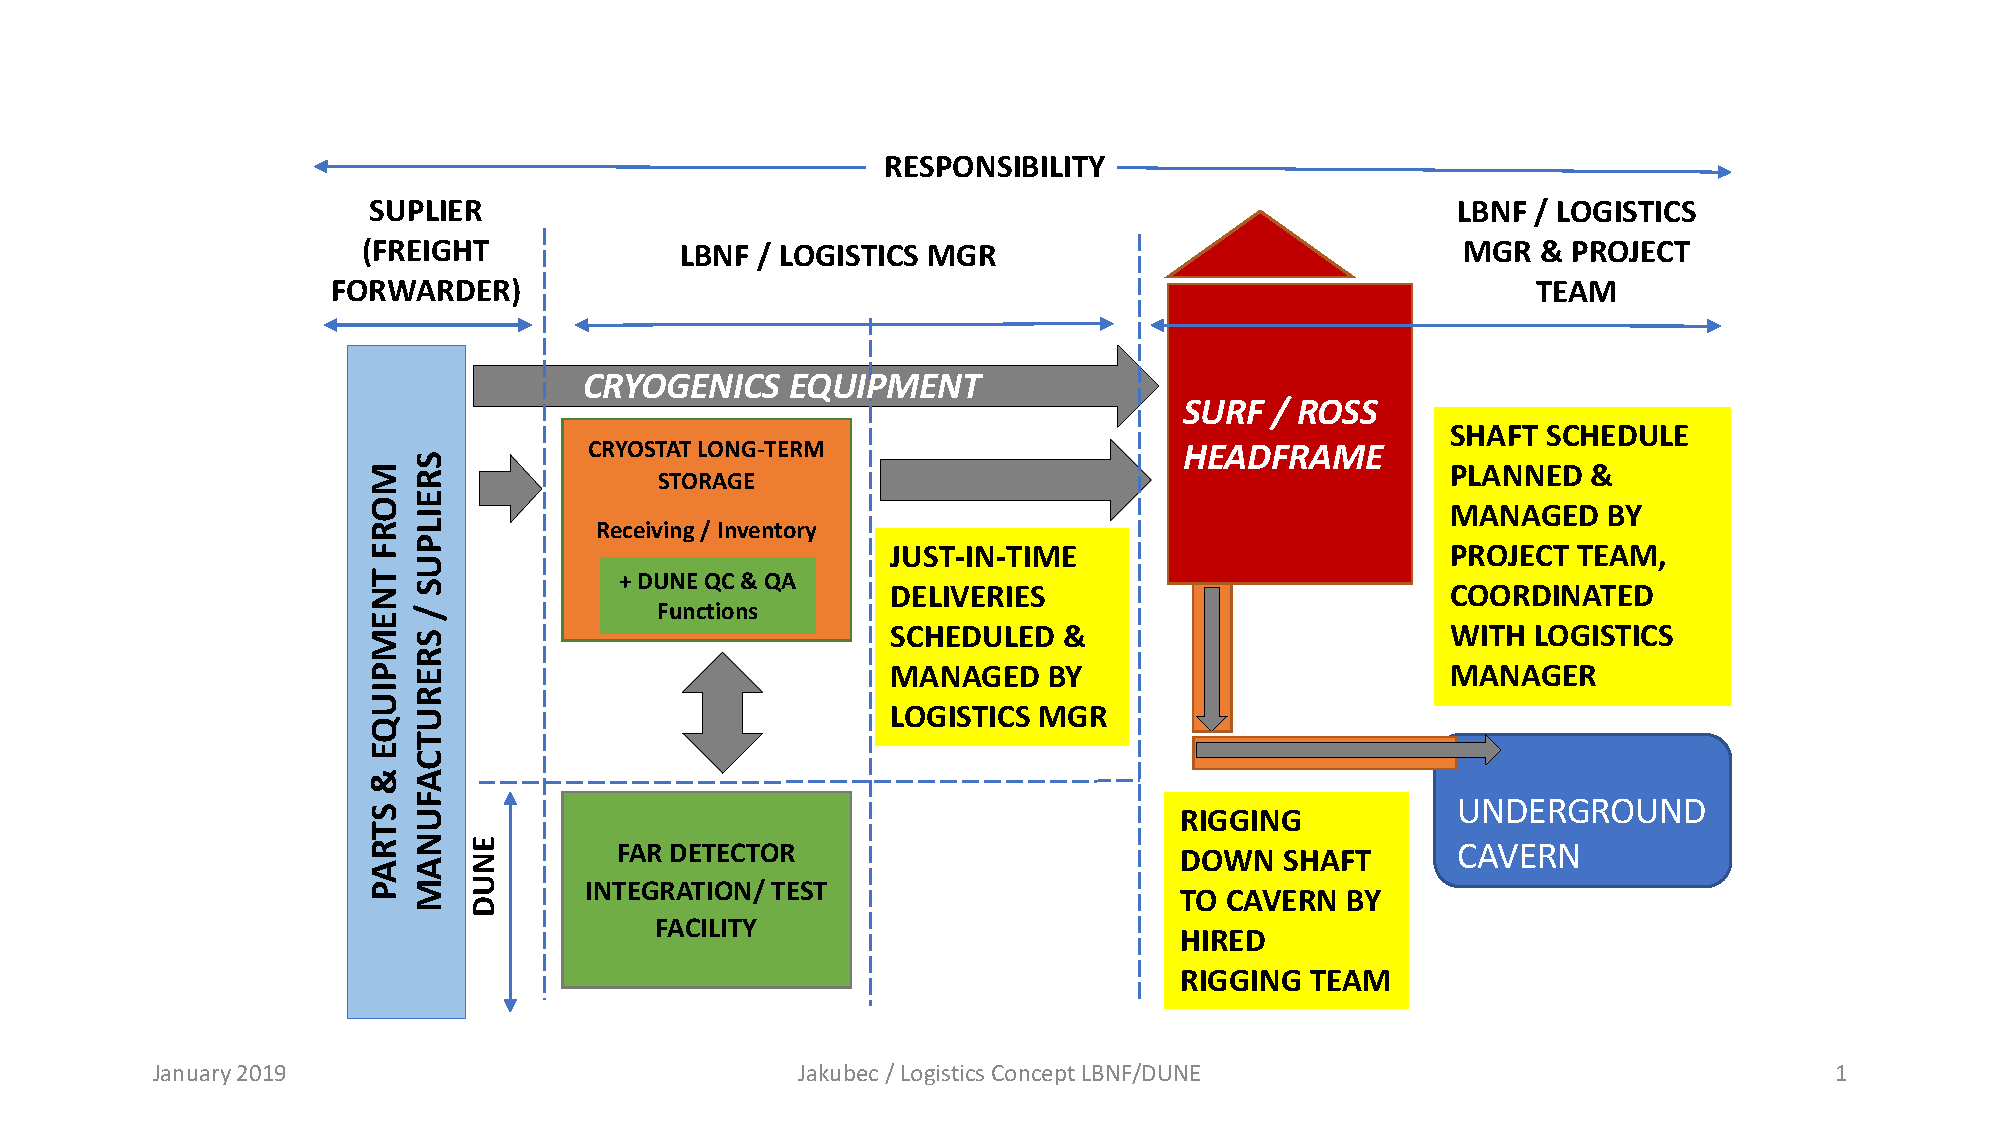
\includegraphics[width=\textwidth]{logistics-material-flow}
\end{dunefigure}

%%%%%%%%%%%%%%%%%%%%%%%%%%%%  
\subsection{Logistics Planning}
\label{sec:fdsp-tc-logPln}

The %\dword{lbnf} and \dword{dune}
\dword{sdsd} logistics team oversees transportation of the cryostat (steel, foam, and membrane), the cryogenics system, the detector \fixme{components? anne} , and all related infrastructure not provided by the \dword{cf}. 
\dword{lbnf} specifically oversees the cryostat and cryogenics system, which are  discussed in detail in the \dword{lbnf} \dword{tdr}; because \dword{lbnf} material dominates the logistics, we present a summary.  
 \fixme{Anne needs to add LBNF TDR ref when available}
The steel structure for a \dword{dune} cryostat requires roughly 1,800 individual steel pieces,  some of which weigh up to \SI{7.5}{t}, as well as \SI{125}{t} of bolts to assemble the steel frame. \fixme{really, 125 t of bolts for one cryostat? No factor of 10 mistake here?}
The internal structure for the cryostat, which includes the foam insulation and the thin stainless steel membrane, requires transporting roughly 4,000 boxes of approximate size  % each roughly 
 1.5 $\times$ 3.5 $\times$ 1.2 m$^3$. 
 %The plan for cryostat installation, at present, calls for all components to be warehoused
 The current plan calls for warehousing all these boxes at the \dword{sdwf} before installation begins. 
%This facility will need to have 
The logistics operation will require roughly $\SI{5000}{m^2}$ of space available here  %to the logistics operation 
approximately two years before installation of the first \dword{detmodule} begins. 
By the time detector components start arriving, most of the cryostat boxes will have been delivered to \dword{surf}, %removed from the \dword{sdwf}, 
leaving ample space for the detector and the cryogenics components. % which are not delivered directly to the Ross Headframe. 
Additional space may be required if the boxes for the second cryostat arrive before  \dword{detmodule} \#1 installation is complete; a few buildings of the required size are available in the general area around \dword{surf}. 

\begin{dunefigure}
[Simplified model of the Ross Cage]
{fig:fdsp-tc-Cage}
{Simplified Ross Cage model and Specifications.}
\parbox{2.1in}{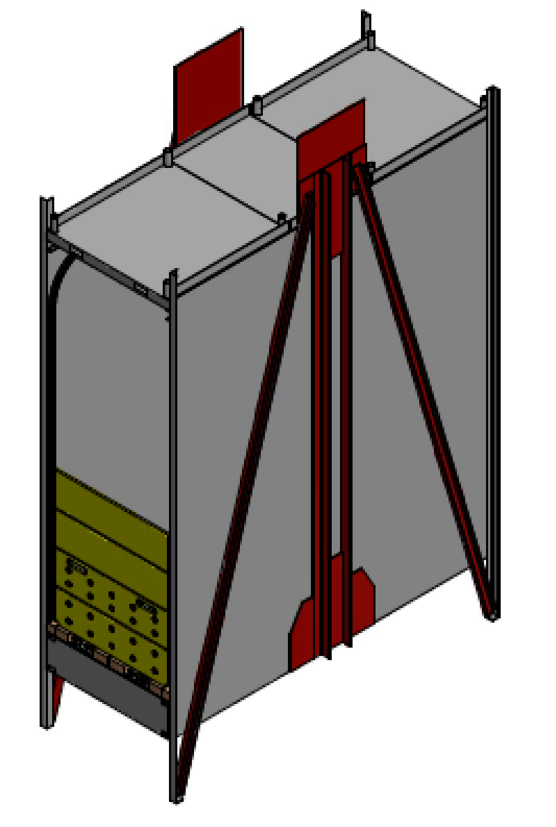
\includegraphics[width=0.3\textwidth]{graphics/Cage-view.pdf}}
\qquad\hspace{10pt}
\begin{minipage}{0.5\textwidth}%
\begin{tabular}{p{3.4cm}p{3.4cm}}        
\multicolumn{2}{c}{Ross Cage Specifications}\\ \toprowrule
Inside height & 3.6 m\\ \colhline
Inside depth  & 3.7 m \\ \colhline
Inside width  & 1.38 m \\ \colhline
Weight limit  &  5,897 kg \\ \colhline
Round trip \newline time & 17 min \newline (incl. unloading) \\ \colhline
\end{tabular}
\end{minipage}
\end{dunefigure}

The \dword{surf} Facility Access Specification~\cite{bib:docdb328} defines the limitations on dimensions and weights for all materials to be transported underground, the most stringent of which are set by the Ross Shaft and Cage. 
It is possible to bring material down the shaft underneath the cage or in the skip compartment  as a slung load, but this is a much slower process and requires careful planning %detailed procedures, and review. 
and review of detailed procedures for each trip. 
The  \dword{apa}s, for example, require this special handling because they are too tall to fit in the cage. 

Most material will be brought underground inside the cage. Figure~\ref{fig:fdsp-tc-Cage} illustrates the new Ross Cage and summarizes its parameters.  
The roundtrip travel time for the Ross cage is 17 minutes (actual travel time is \num{3.6} minutes each way), dominated by loading and unloading time.  
Slung loads will require more than an hour round trip.



The Ross Headframe has no loading dock so careful planning of material loading and unloading of shipments is required. 
All materials %transported to it 
must arrive on a flatbed or curtain-sided chassis, %where a forklift can unload the items. 
and a forklift will be available for unloading. 
% ALREADY SAID The logistics team coordinates all deliveries from the \dword{sdwf} to the headframe, and the \dword{cf}-\dword{cmgc} coordinates all transport from there down the shaft.  
% ALREADY SAID Most material will be delivered first to the \dword{sdwf}, where a central inventory system will capture data about the shipments.  
All deliveries, either from %this warehouse 
the \dword{sdwf} or direct to the Ross Headframe, require (1) coordination with the \dword{sdsd} logistics organization, and (2) minimum two weeks prior notice, per an advance delivery plan.  
%The logistics team 
Logistics will provide a shipping manual \cite{bib:docdb13954} to \dword{dune} institutions that  
%It 
will specify guidelines %for provision of 
on required shipping data and %for 
cargo consignment such that the logistics organization can monitor shipping progress and no delays occur due to incomplete or missing documentation. 


In \dword{pdsp}, delays in shipping and customs resulted in up to three weeks delay in the arrival of some parts, which necessitated significant re-planning of the installation work.  To prevent this from becoming a much larger problem in \dword{dune}, we plan a minimum one month buffer of materials. This buffer will allow advance planning for the underground work, with confidence that all materials will be available as needed. 

Sufficient space must be made available at the \dword{sdwf} and in the underground area  to house this material.
The \dword{sdwf} staff will de-consolidate or consolidate arriving cargo into appropriately sized boxes and crates, as needed, for delivery to \dword{surf}, to make the most efficient use of available trucks and the Ross Shaft. 

\begin{dunefigure}[Planned usage of underground space during installation setup]{fig:fdsp-tc-setup}
  {CAD image showing the empty half of the north cavern as used during the installation setup phase of the first \dword{detmodule}.  Half of this empty space will be used for the cryostat work and half for storage of the detector infrastructure. The material shown outside the cavern must be stored in the \dword{sdwf}.}
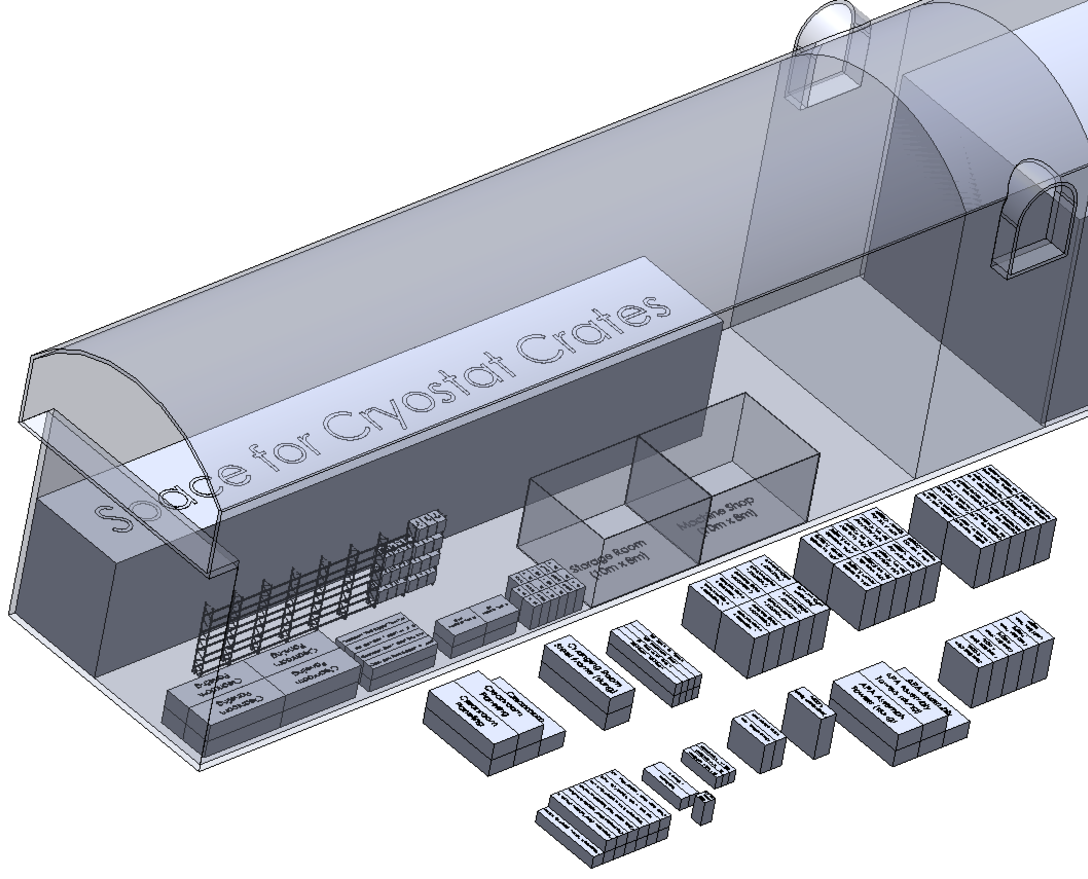
\includegraphics[width=.9\textwidth]{Material-Setup}
\end{dunefigure}


To determine the %\dword{dune} 
storage space requirements and how much hoist time must be dedicated to \dword{dune}, a detailed inventory of all  \dword{dune} detector equipment and infrastructure is needed. 
A complete list of materials has been solicited from all consortia and technical coordination. 
The entries in the inventory spreadsheet are organized as \textquotedblleft loads\textquotedblright \ for the Ross shaft where a load is a crate or set of boxes that will be transported underground in one trip, either in the cage or as a slung load~\cite{bib:docdb8426}. 
Information captured in the load spreadsheet includes the number of  
trips, type of trip (slung load or cage), package dimensions, weight, and type of package (crate, pallet, box, or carton). 

The load list at present predicts 1,600 hoist trips and approximately two  months of cage time, most of which is spread over one year. 
Detector installation (see Figure \ref{fig:high-level-schedule}) for the \dword{spmod} will span two years, so we divide the logistics planning into three phases: (1) the \dword{cuc} setup phase, (2) the installation setup phase, and (3) the detector installation phase. 
For each phase, a \threed model was generated to show how much material can be stored underground outside the work area and how much material must be stored %on the surface
at the \dword{sdwf}, thus setting the surface space requirements. 
%These models set the requirements for the logistics on the surface. 
The phase with the largest amount of material to transport is the installation setup phase.  
Figure~\ref{fig:fdsp-tc-setup} shows the model of the underground area and the required boxes for surface storage for %the first third of the setup. 
%This represents 
the first month of this phase. %installation setup and shows that r
Roughly $\SI{1000}{m^2}$ of warehouse space will be needed for \dword{dune} at this time.  The \dword{sdwf} will also need space to store up to 150 \dword{apa}s, 
adding another $\SI{700}{m^2}$. % to the 1,000 m$^2$. 


%%%%%%%%%%%%%%%%%%%%%%%%%%%%
\subsection{Logistics Quality Control}
\label{sec:fdsp-tc-log-qaqc}


 
The \dword{pdsp} experience offers a couple of significant lessons regarding logistics.

\begin{enumerate}
\item A central inventory system is essential for tracking  shipments.
\item It is important to avoid delays in shipping because they prevent installation work from  proceeding as planned. 
\end{enumerate}

The central inventory system  implemented at the \dword{sdwf}  and minimum one-month material buffer are the plans we have in place to prevent repetition of the \dword{pdsp} schedule problems. % we experienced with \dword{pdsp}.   
The full list of lessons learned from \dword{pdsp} is in~\cite{bib:docdb8255}. 

We do not foresee any component testing at the \dword{sdwf}, so the scope of the \dword{qc} work there is limited to two functions: 
The \dword{sdsd} logistics organization in coordination with the %facility  
the \dword{sdwf} will inventory all received shipments and  ensure that all materials fit in the Ross Cage, or if a slung load is needed, that the necessary procedures are in place and approved before any material is transported to the Ross Headframe.  
%The logistics provider will inventory all received shipments. \dword{jpo} representatives will verify that no obvious damage occurred in transport.
\dword{jpo} representatives will verify that no obvious damage occurred in transport. 

The contribution-in-kind model of this project complicates logistics oversight and inventory control %as 
since components will be delivered from many institutions and from different countries. 
%Similarly, the \dword{qc} information gathered during production and testing must be gathered from and accessible to all collaborators. 
Similarly, during production and testing, \dword{qc} information must be gathered from and made accessible to all collaborators. 
Because of the complexity of the project and the different requirements for \dword{qc} and logistics oversight, two different databases will be used. % for the two functions. 
A commercial \dword{wms} will control the inventory process at both the \dword{sdwf} (items both received and shipped) and at \dword{surf} (items received at the Ross Headframe). A  separate database, the \dword{dcdb}, will %be used to 
store testing and other \dword{qc} data, e.g.,  shipping reports and any reported damage. 
The \dword{wms} will need to provide location and  \dword{qc} information to the \dword{dcdb}, which will ultimately archive %the construction 
both sets of data. The \dword{dcdb} has yet been designed.

Until materials arrive at the \dword{sdwf} (or \dword{surf} if directly shipped), the contributors' freight forwarding system will control the logistics supply chain, which will depend on the contractual circumstances and the contributor's choice. 
However, assuming the shipment is consigned as outlined in the  shipping manual (so that the %\dword{sdsd} 
logistics organization has access to the shipping data),  logistics will monitor the cargo progress and step in if a problem arises. 
%The \dword{sdwf} will be the ultimate point of capture for all the materials, except possibly for elements of the cryogenics system, given its special contractual requirements.
% PREV SENTENCE IS UNCLEAR AND MUDDIES THE WATERS. I THINK THE NEXT SENTENCE CAPTURES WHAT YOU'RE TRYING TO SAY. ANNE
% ALREADY SAID ABOVE. ANNE The \dword{wms} will control basic receiving, inventory control, and shipping status for all components, parts, and equipment delivered to the \dword{sdwf}.

% ALREADY SAID ABOVE. ANNE The \dword{dcdb} will be the central repository for all \dword{qc} data. All relevant \dword{qc} data related to logistics must be transferred from the \dword{wms} to the \dword{dcdb} where it is archived. This information includes shipping reports and any reported damage. 
The \dword{qc} and shipping data flow is shown in Figure~\ref{fig:logistics-data-and-mat-flow}.

 


\begin{dunefigure}[QC and shipping data flow diagram for logistics]{fig:logistics-data-and-mat-flow}
  {\dword{qc} and shipping data flow diagram for the \dword{lbnf} and \dword{dune} logistics.}
 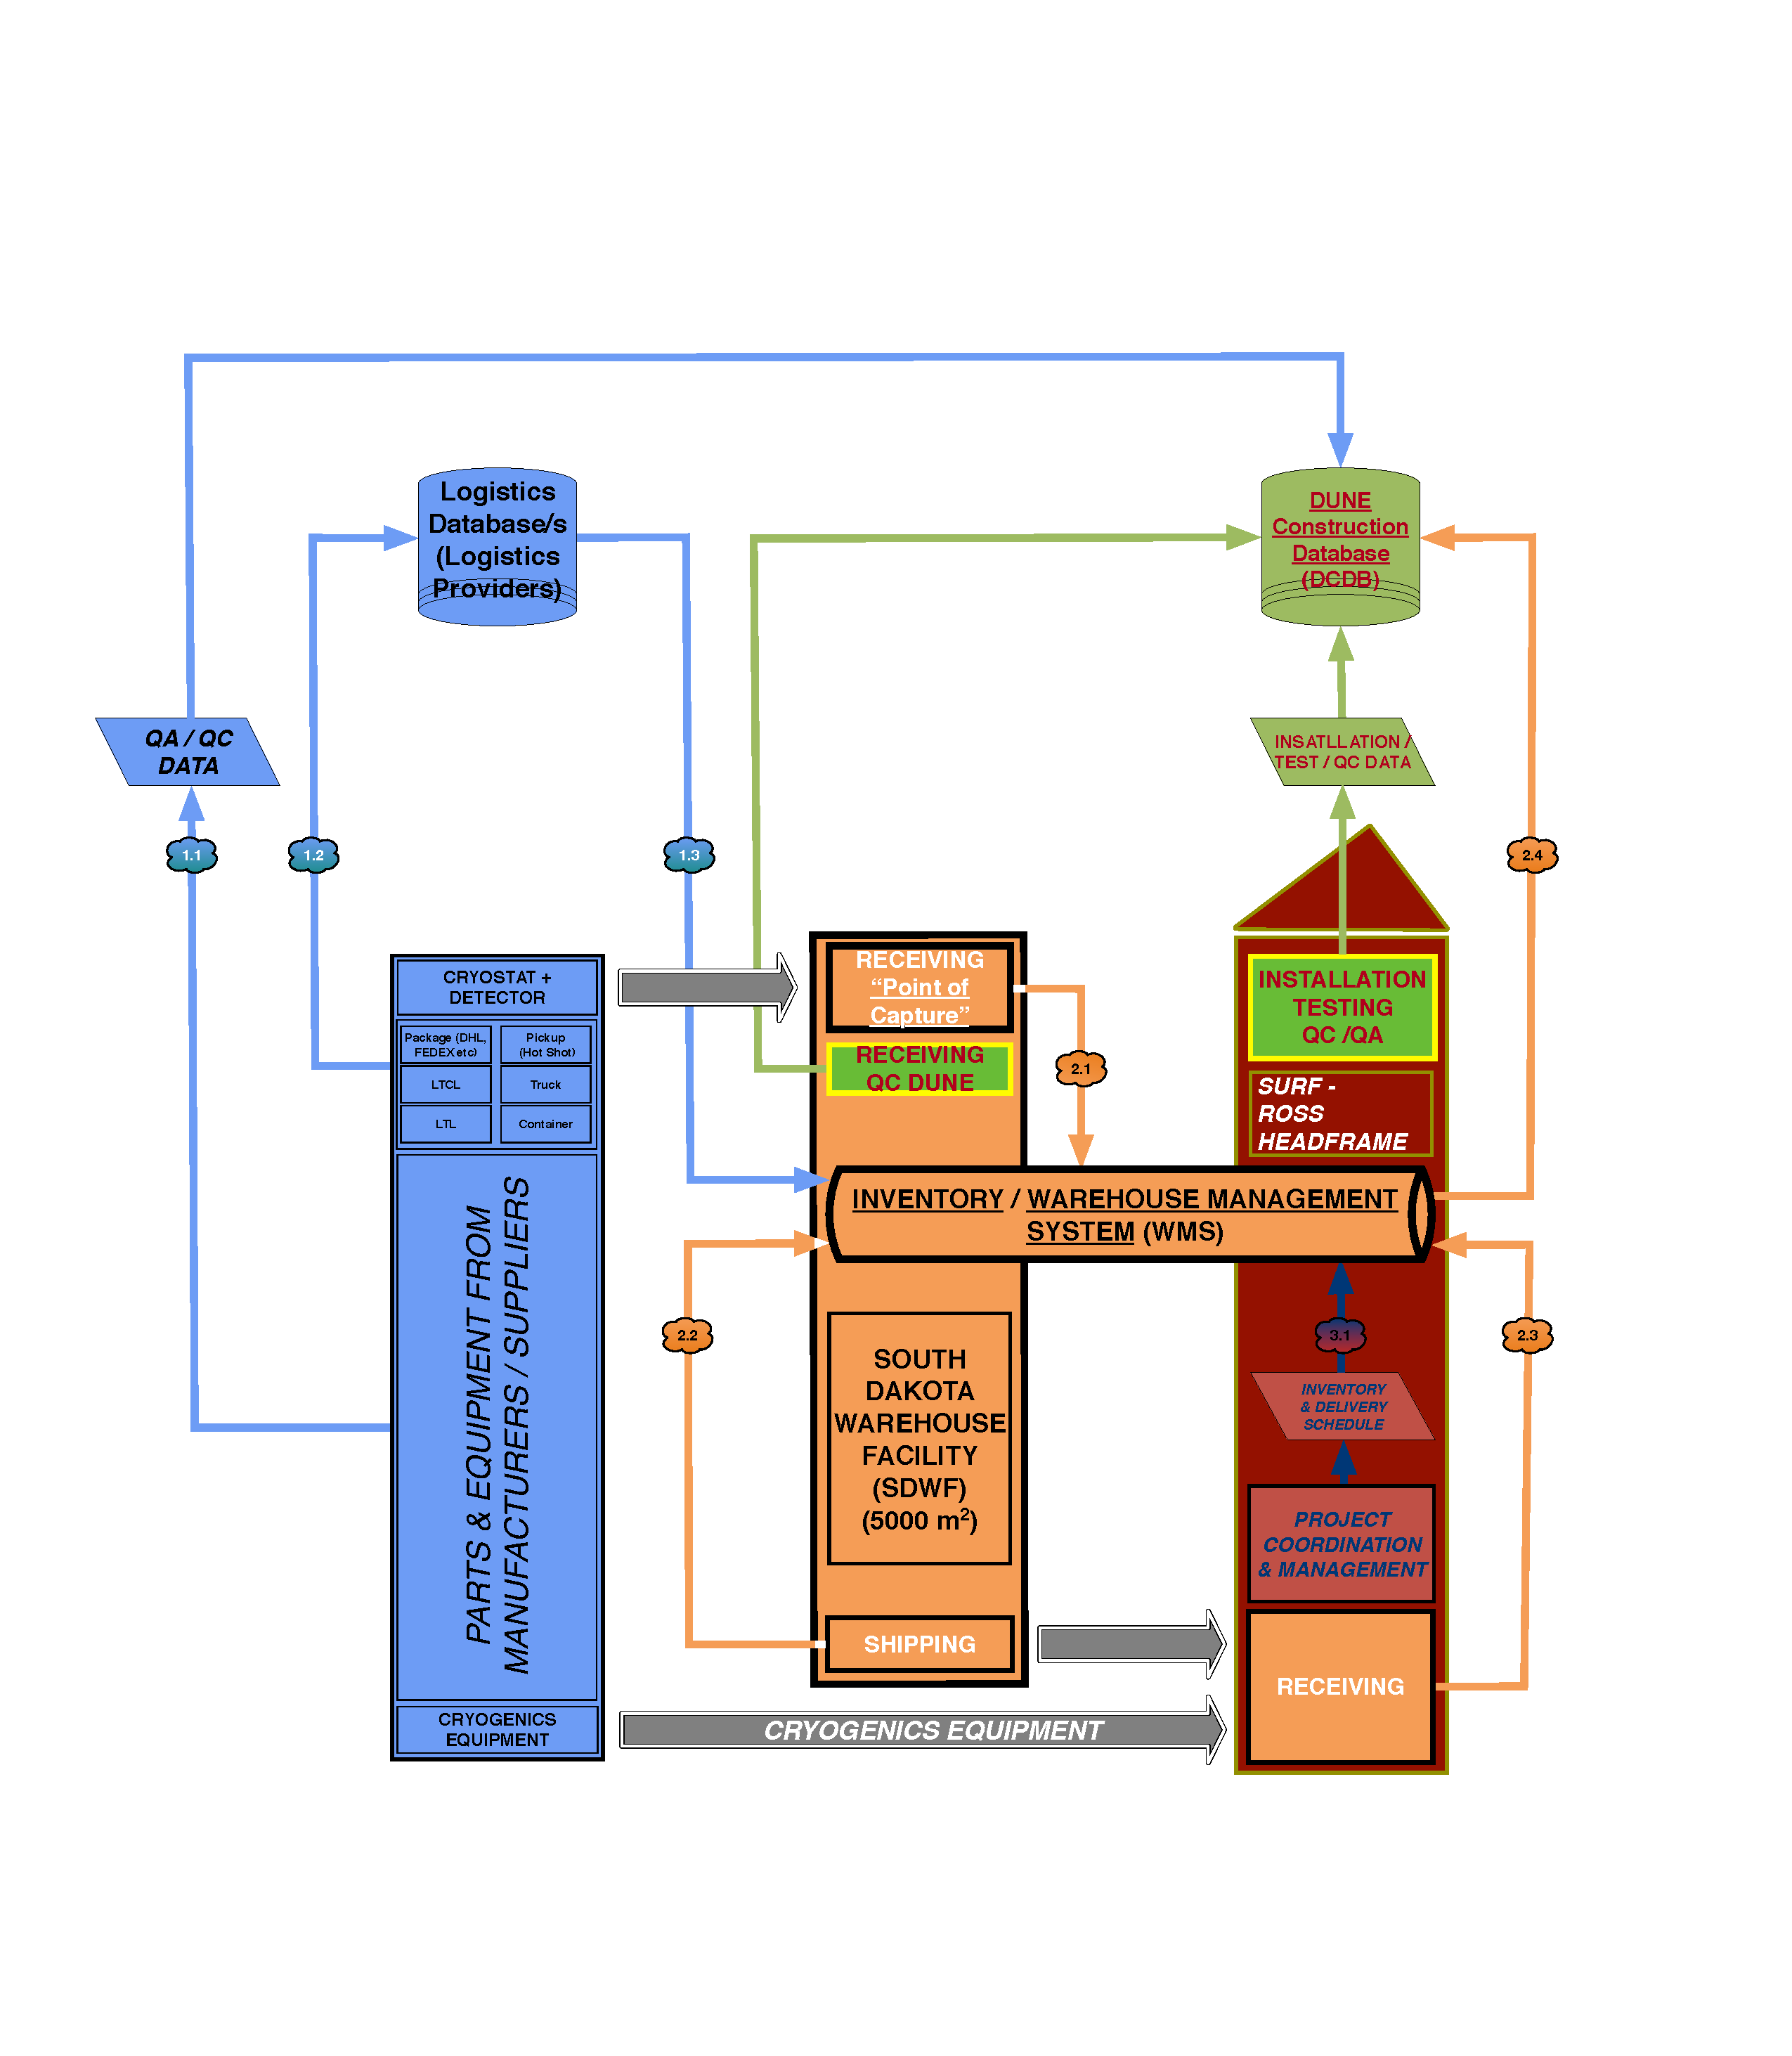
\includegraphics[width=\textwidth]{logistics-data-and-mat-flow}
\end{dunefigure}

 
The \dword{jpo} installation management team will provide a shipping (supply) report to the \dword{sdsd} logistics organization and \dword{sdwf} for scheduling delivery of parts and equipment two weeks in advance of the required delivery date. 
All %shipments 
deliveries will be inventoried upon receipt at the Ross Headframe in the \dword{wms}. 




%%%%%%%%%%%%%%%%%%%%%%%%%%%%
\subsection{Logistics Safety}
\label{sec:fdsp-tc-log-safety}

\fixme{from Ladia 16 Apr}
The \dword{sdwf} will be managed and operated by an independent contractor under the supervision of the %Far Site 
\dword{sdsd} logistics manager. 

The facility will be operated under the contractor's \dword{esh} program that has to conform to federal regulations and will be reviewed by \dword{fnal}'s \dword{esh} management prior to entering a contractual relationship.

\begin{comment}
\fixme{talk with Mike A, Niehoff, Bill Miller}
%The \dword{lbnf}/\dword{dune} logistics facility is operated by \dword{sdsd}  as a Fermilab facility, but because of the international connections, we also follow CERN HSE, Fermilab ES\&H, and \dword{surf} ES\&H regulations.  Work is in progress to combine the three into a coherent list of codes and requirements. The \dword{dune} Project ES\&H Coordinator has overall ES\&H oversight responsibility for the \dword{dune} Project.  This person coordinates any activities and facilitates the resolution of any issues that cut across various divisions and institutions and subject to the requirements of the \dword{doe} Workers Safety and Health Program, Title 10, Code Federal Regulations (CRF) Part 851 (10 CFR 851). These requirements are promulgated through the Fermilab Directors Policy Manual and Fermilab ES\&H manual (FESHM), which align with the \dword{surf} ES\&H Manual.  Using the NOvA Far Detector Laboratory as a guideline for remote facilities, several other key documents guide the Logistics Center Safety Program.  The Building Safety Plan combines all building specific documents in a single folder:
The \dword{sdwf}  is operated by \dword{sdsd}  as a \dword{fnal} facility, but because of the international collaboration, we  follow \dword{esh} regulations from \dword{cern} and \dword{surf} in addition to \dword{fnal}'s.  Work is in progress to combine the three into a coherent list of codes and requirements. The \dword{dune} Project \dword{esh} Coordinator has overall \dword{esh} oversight responsibility for the \dword{dune} Project.  This person coordinates any \dword{esh} activities and facilitates the resolution of any issues that are subject to the requirements of the \dword{doe} Workers Safety and Health Program, Title 10, Code Federal Regulations (CRF) Part 851 (10 CFR 851), and that cut across various \dword{fnal} divisions and collaborating institutions. These requirements are promulgated through the \dword{fnal} Director's Policy Manual \fixme{ref} and \dword{fnal} \dword{esh} manual (FESHM\cite{feshm}), which aligns with the \dword{surf} \dword{esh} manual.  Using the \dword{nova} Far Detector Laboratory as a guideline for remote facilities, several other key documents guide the Logistics Center Safety Program. \fixme{I don't think this should be capitalized; certainly not without an accompanying reference. Anne} The Building Safety Plan \fixme{ref} combines all building specific documents in a single folder:

\begin{enumerate}
\item	Fire Safety and Building Emergency Evacuation Plan, which includes the fire evacuation plan, fire safety plan,  lockdown plans, and the site plan;
\item	Hazard Analysis document, which describes all typical hazards and their mediation %including 
procedures; 
\item	%SDS: 
Safety Data Sheets (SDS), 
\item	Respiratory Plan, as required for chemical or ODH hazards, and 
\item	Training Program, which covers required certifications and  training records.
\end{enumerate}
\fixme{ref all when available}
The current Technical Coordination Facilities Management Plan \fixme{ref} specifies a safety officer for the \dword{jpo} including the logistics facilities. This safety officer facilitates training, writes hazard analysis documents, runs weekly safety meetings, and keeps documentation records on materials-handling equipment and personnel information such as training, \dword{ppe} and other qualifications. 
\end{comment}






%%%%%%%%%%%%%%%%%%%%%%%%%%%%%%%%%%%%%%%%%%%%%%%%%%%%%%%%%%%%%%%%%%%%
%\section{Integration and Test Facility (ITF)}
%\label{sec:fdsp-tc-itf}

\section{Integration and Test Facility (ITF)}
\label{sec:fdsp-tc-itf}



The components of the \dword{dune} detectors will be manufactured in several different countries. 
Many of the parts can be reasonably shipped to the logistics warehouse and then underground where it can be installed. 
However, the  \dword{ce} and the \dwords{pd} are tightly coupled to the \dword{apa}s. 
The wires and filters on the d\dword{apa}s form part of the electronics circuit, and the photon supports and cabling are built into the \dword{apa}s. 
Integrating the \dword{ce} and \dword{pd}s into the \dword{apa}s is a huge task, and the risk of damaging the components is significant. Thus, we plan to integrate the components as early in the process as possible and then thoroughly test the complete assembly.
To avoid creating integration testing facilities at each factory, one central facility will be established in South Dakota near the \dword{surf} site  (within an hour's drive). 
The \dword{apa}s, \dword{ce}, and \dwords{pd} modules will arrive in this \dword{itf}, undergo initial tests, be integrated, and then undergo a set of warm tests. 

Because the \dword{ce} will be available approximately two years before installation begins, the \dword{itf} must be available on the same time scale. Other components are, in fact, available earlier. 
Table \ref{tab:specs:just:SP-TC} summarizes the specifications for the \dword{itf};  
the relevant specifications involve the quality of the cleanroom and the UV light filtering for the \dwords{pd}.



%\begin{dunetable}
%[ITF Specifications]
%{cc}
%{tab:tcps-itf-spec}
%{Summary of the high level specifications for the ITF. %The building requirements are covered separately in a separate section.}
%Parameter & Specification \\ \toprowrule
%Cleanroom & The ITF cleanroom shall meet ISO-8 standard per ISO-14644 \\ \colhline
%Filtered Lights & <520 nm for long exposure and <400 %for exposures less than 2 weeks \\ 
%\end{dunetable}



%%%%%%%%%%%%%%%%%%%%%%%%%%%%
\subsection{APA-CE-PD Integration}
\label{sec:fdsp-tc-itf-integ}

\begin{dunefigure}[ITF cleanroom layout]{fig:fdsp-tc-itf-clean}
{Conceptual layout of the cleanroom for APA-CE-PD integration and testing.}
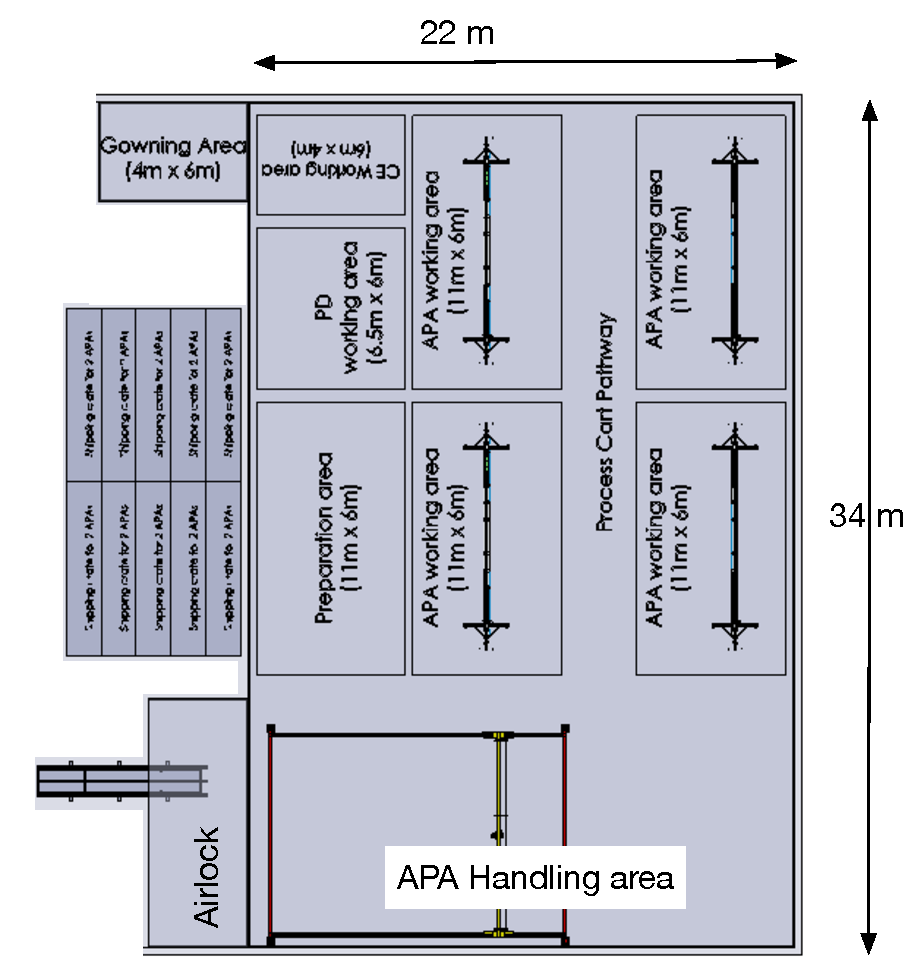
\includegraphics[width=0.8\textwidth]{itf-cleanroom-v2}
\end{dunefigure}

Most the work in the \dword{itf} must be done in a cleanroom environment to protect the components from dust and unfiltered light. The cleanliness requirement for the detector components is ISO-8 which corresponds to filtered air with clean lab coats, clean shoes, and hair nets. 
To protect the photon detector's \dword{wls} coating, the lights must be filtered to remove frequencies below 520nm.\cite{LBNE-docdb-8348} Figure \ref{fig:fdsp-tc-itf-clean} shows one possible layout of the cleanroom.
Materials enter the \dword{itf} cleanroom through the materials airlock. This area must be sufficiently large to accommodate \dword{apa} transport boxes and allow workers to move around the box to remove the dirty shipping layer and prepare the equipment for transport into the cleanroom. 
Other materials will also be brought into the cleanroom through the airlock, but they will need much less space than the \dword{apa} crates. Figure \ref{fig:fdsp-tc-itf-clean} shows an \dword{apa} transport box being moved into the airlock on the lower right.
The \dword{ce} and \dword{pd} equipment will be moved to their own work areas. 
Here the components are unpacked and tested before integration into the \dword{apa}. 
The tests performed are described in more detail in the \dword{qc}/\dword{qa} section below. 

The \dword{apa}s enter the cleanroom through the airlock and initially go to the \dword{apa} handling area where an overhead workstation or gantry crane will be available. 
The \dword{apa} will then be removed from the transport box and mounted to a process cart that can rotate the \dword{apa} horizontally. The process cart will be pushed to one of the four \dword{apa} integration areas where they are prepared for the installation of the \dword{ce} and \dword{pd}. 
During the integration process, the \dword{apa} will be held horizontal and the \dwords{pd} will be inserted into the sides while the \dword{ce} boxes are mounted to the end of the \dword{apa}. 
After integrating the components, the system will be tested and then moved back to the handling area and boxed for shipping to the logistics center for storage.  

All detector  components will arrive at the \dword{itf} either from the logistics facility or directly from the factories. Sufficient space will be needed inside the \dword{itf}, but outside the cleanroom, to store the material needed for several weeks as well as a few of the integrated \dword{apa} boxes. Additionally a changing room is needed, so workers can change into clean clothes and shoes. The changing room should have a capacity sufficient for the 10-20 workers needed in the cleanroom. 

%%%%%%%%%%%%%%%%%%%%%%%%%%%%
\subsection{ITF QA/QC}
\label{sec:fdsp-tc-itf-qaqc}
Extensive testing of the detector components will be performed inside the \dword{itf} facility as the APA-PD-CE integration takes place. These tests are a vital part of the quality control process for \dword{dune}. Details of the tests for each of the components are described below.

\subsubsection{APA}
The \dword{apa} will be unpacked from the transport box, installed on the process cart, and the protective shields removed to allow a detailed visual inspection. Then it will be transported to the integration area, where it will be held horizontally. The main test to be performed at this stage, i.e., before integration with the \dwords{pd} and \dword{ce}, is tension measurement. Ideally, all wires would be measured to ensure that no changes occurred during shipping. The limiting factor for the tension measurement will be time. In the current plan, approximately 350 wires, representing 10$\%$ of the total, will be measured, which will take 3 shifts with 2 people. All the measured values will be stored in the wire \dword{qc} database. In the current plan, the tension measurement will be performed using a laser, the same method used at the production site. This method uses a laser focused on individual wires. By plucking the wire to induce a vibration, a photodiode under the wire records the frequency of vibration, which directly translates into the tension value. While this method is robust and has been extensively used by \dword{lartpc} experiments, it is very time consuming. An alternative method, using electrical signals, is currently under development and could replace the laser method, potentially allowing all \dword{apa} wires to be measured at the \dword{itf} in less time.

The current requirement for tension values are 6$\pm$1 N. Wires measuring outside this range will be removed from the \dword{apa}. Note that the exact tolerance is currently under study with \dword{protodune} data to ensure the required acceptable range; otherwise, a channel may have to be removed.

The last test performed to ensure the quality of an \dword{apa} is the wire continuity. This checks that all wires are still intact and properly connected to the readout boards. This test can easily be done once the \dword{ce} is installed (see next sub-section).    
\subsubsection{Cold Electronics}
The \dword{qa} for the \dword{ce} is described in the \dword{ce} chapter.

\subsubsection{Photon Detectors}

\dwords{pd} will arrive at the \dword{itf} in custom designed crates.  Each crate will contain the ten photon detector modules required for a single \dword{apa}.  
Each \dword{pd} comes individually packaged in a static-resistant sealed plastic bag, filled with clean dry nitrogen.

Before each \dword{pd} is integrated into an \dword{apa}, it is removed from its shipping bag and inspected visually. 
Modules passing this initial inspection are then loaded into the optical scanner for operational testing.

The \dword{pd} optical scanner tests the operation of the photosensor readout chain to ensure all electrical connections are operational and also measures light-collection performance at several positions along the length of the module.  
Duplicate identical optical scanners are used at the module assembly facility, where a scan is the last \dword{qc} test before the module is shipped to the \dword{itf}; the module is tested again immediately before installation, allowing a sensitive test for any changes in module performance due to shipping or storage.  
This technique was used successfully in \dword{pdsp}, and will be replicated for \dword{dune}.

The optical scanner consists of a light-tight box, approximately \num{2.5}m long, with a \num{0.75} $\times$ \num{0.75}m cross section. 
The box is fabricated of aluminum and acts as a Faraday cage to minimize electrical interference with measurements. 
In the \dword{dune} configuration, two \dword{pd} modules to be tested are inserted into the station through slots on the face of the box, guided by support rails of the type used in the \dword{apa}s, representing a final mechanical check of the dimensions of the module.  
Electrical connection to the module uses an electrical connector identical to the ones in the \dword{apa} frames, allowing a final check of that crucial interface.
Following insertion into the scanner, the insertion slots are closed and optically sealed, and the scan begins. 
\dword{dune} \dword{pd} readout electronics are used to bias and read out the module photosensors, while a UV LED is scanned along the length of the modules by an automated stepper-motor driven translation stage.  
Measurements of the detector responses are made at 16 positions along the length of the module (on two sides for double-sided \dword{pd} modules), checking the performance of each of the dichroic filters. 
The response is compared to that measured in the assembly facility. 
Figure \ref{fig:fdsp-tc-pds-scanner} shows the scanner used to test the \dword{pdsp} photon detectors.


\begin{dunefigure}[Photon detector scanner]{fig:fdsp-tc-pds-scanner}
{Picture of the scanner for operational tests of the \dword{pd} modules before the modules are inserted into the \dword{apa}s.} 

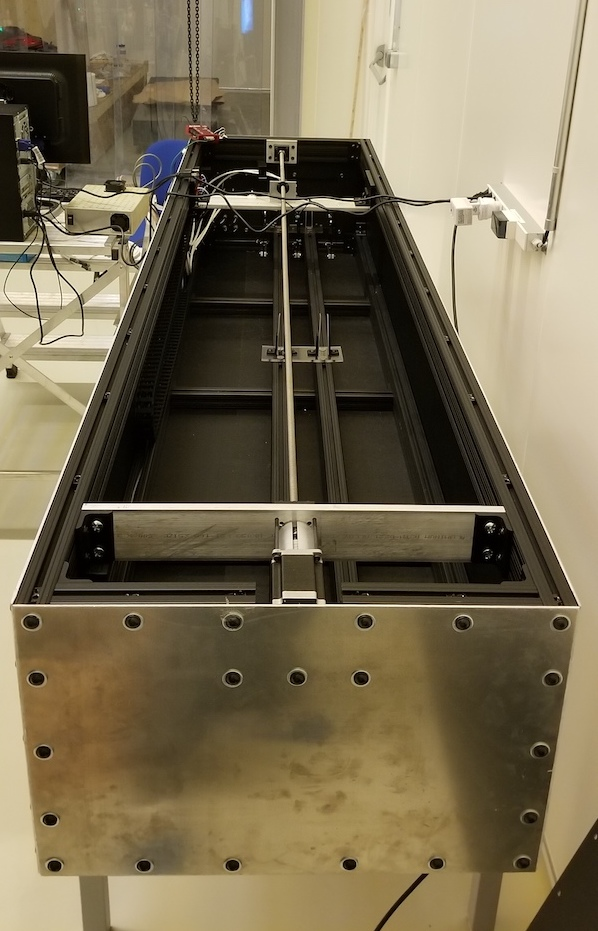
\includegraphics[height=.60\textheight, angle=0]{pds-scanner}
%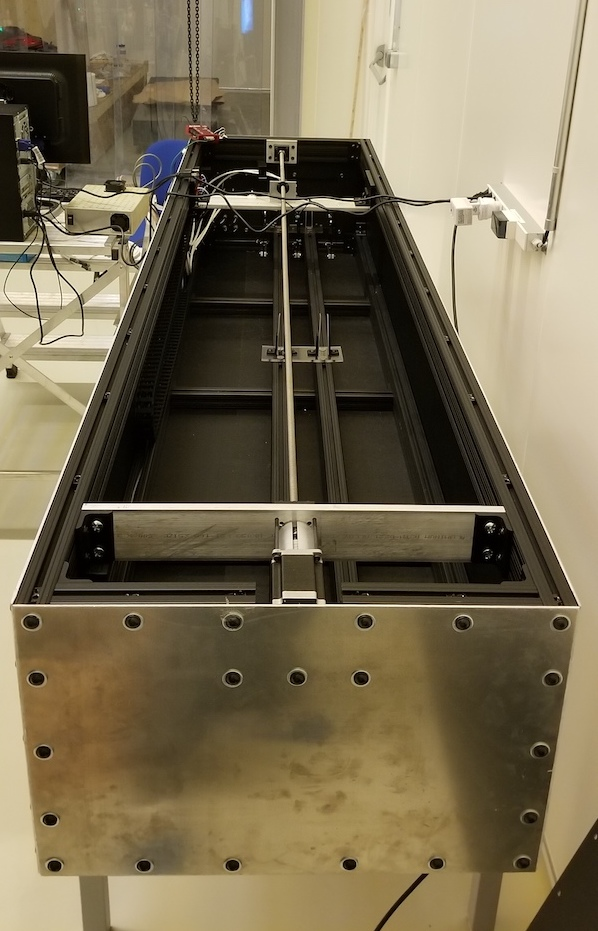
\includegraphics[width=1.0\textwidth, angle=-90]{pds-scanner}
\end{dunefigure}

Photon detector are inserted into the \dword{apa}s immediately follows optical scanning.  
Modules are inserted onto the \dword{pd} support rails; the connection to the cable harness, which is pre-installed in the \dword{apa} before wire wrapping, is automatic as the module is inserted.   
Immediately after the module is inserted, an electrical continuity check ensures continuity between the \dword{pd} module and the \dword{pd} cable end connector where it exits the end of the \dword{apa}.



%%%%%%%%%%%%%%%%%%%%%%%%%%%%
\subsection{Building Requirements and Infrastructure}
\label{sec:fdsp-tc-itf-req}
The \dword{itf} building requirements are summarized in DocDb 11500.\cite{bib:docdb11500} The building to be used as the \dword{itf} has not yet been designated. To help identify or design the \dword{itf} building, a set of requirements were drafted. The requirements document defines the spaces needed for integration work but does not specify the final layout of the cleanroom. This will allow cleanroom spaces to be configured as part of building footprints as candidate buildings are identified. Because the building has not been designated, the cleanroom layout shown in Figure \ref{fig:fdsp-tc-itf-clean} should be taken as a concept; the final layout may change depending on the footprint of the building chosen as the \dword{itf}. The building requirements document\cite{docdb-11500}  defines the minimum spaces needed for all operations inside the \dword{itf} cleanroom. It also defines the space needed for the coldbox and the related cryogenic system, and it provides guidance for the space needed for material storage outside the cleanroom. It also establishes requirements for power and other general needs. Some requirements depend on the location of the building and the facilities available in the area. For example, office space for 20 scientists working in the \dword{itf} will be needed in the area but would not necessarily need to be in the \dword{itf} building itself if other local options are available. Some local machining facilities also fall into this category. 

%%%%%%%%%%%%%%%%%%%%%%%%%%%%
\subsection{Safety}
\label{sec:fdsp-tc-itf-safety}

Information on \dword{itf} safety is identical to what is listed in Section 1.1.4 (Logistics Safety) because the \dword{itf} is also operated by SDSD as a Fermilab facility.    If the \dword{itf} and logistics facility are near each other, one safety officer can be shared by the two sites.    

%%%%%%%%%%%%%%%%%%%%%%%%%%%%
\subsection{Cost, Schedule and Risk Analysis}
\label{sec:fdsp-tc-itf-cost}

\fixme{Add costs when they are available}

{\bf ITF Time Line and APA Integration Schedule}
The time line for starting up the \dword{itf} is 2022 when \dwords{pd} and \dword{ce} are available to integrate into the \dword{apa}s.  This allows two years to integrate \dword{apa}s
before installation begins. This schedule has the advantage of allowing all integrated components to be tested as soon as possible, minimizing any schedule risk if problems occur. The integration team size would be smaller because the time-scale is longer, reducing labor costs. Because the schedule for integrating the components will take less time, we can start integration closer to one year before detector installation. 

Using four work stations and working with only a day shift, installing an \dword{apa} pair should take approximately nine shifts as shown in Figure \ref{fig:ITF-Schedule}.

\begin{dunefigure}[Schedule APA Integration in ITF]
{fig:ITF-Schedule}
    {ITF-Schedule}
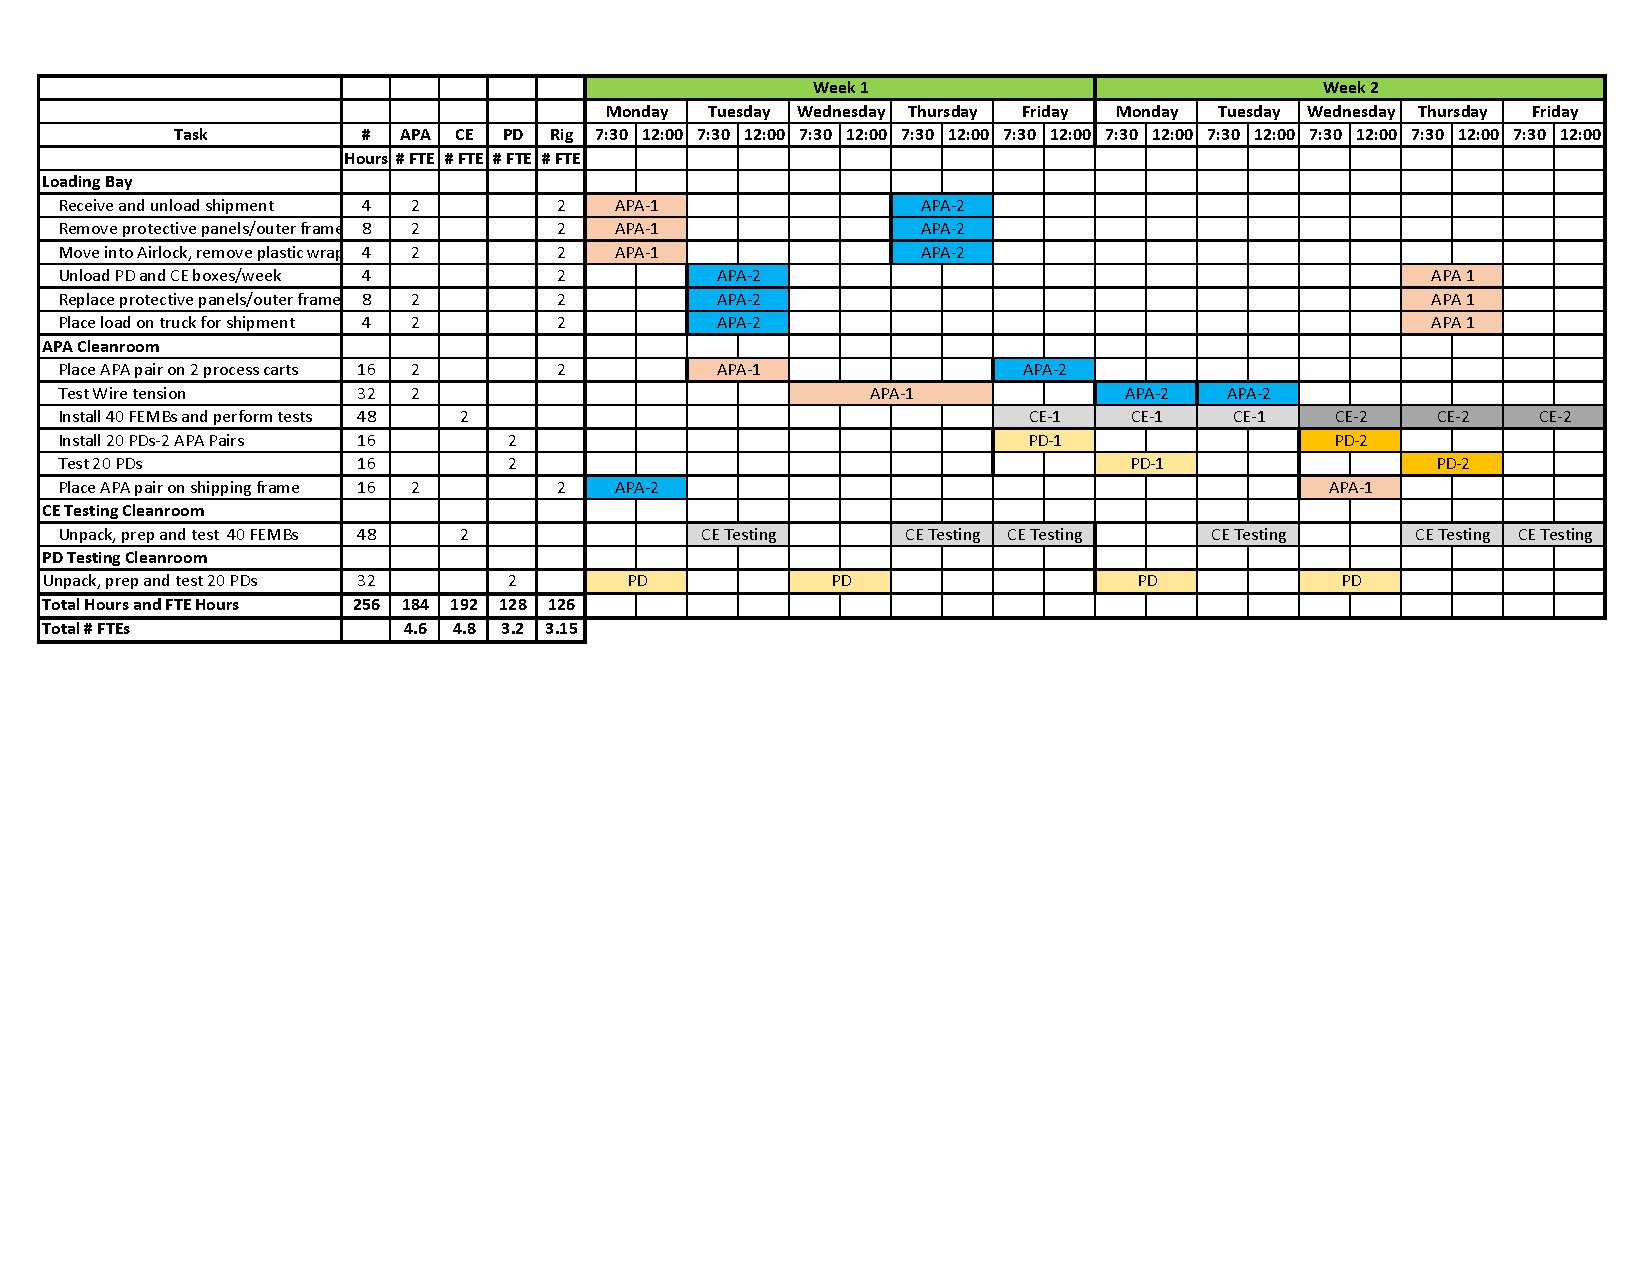
\includegraphics[width=0.98\textwidth]
{ITF-Schedule.pdf} 
\end{dunefigure}


\fixme{use templates from cost-risk-sched.tex file. Anne}


%%%%%%%%%%%%%%%%%%%%%%%%%%%%%%%%%%%%%%%%%%%%%%%%%%%%%%%%%%%%%%%%%%%%
%\section{Infrastructure}
%\label{sec:fdsp-tc-infr}
\section{Detector Infrastructure}
\label{sec:fdsp-tc-infr}


The  \dword{jpo} will provide the infrastructure needed to install the \dword{spmod}. The major items, described below, include the \dword{dss}, the electronics mezzanine on the cryostat roof (including racks), cable trays, an underground cleanroom with appropriate installation equipment, piping inside the cryostat, and \coldbox{}es with associated cryogenic supply. 

Other items, not described here but also in the \dword{jpo} scope, include a small machine shop, scissor lifts, rigging equipment, hand tools, diagnostic equipment (including oscilloscopes, network analyzers, and leak detectors), local storage with some critical supplies, and \dword{ppe}.  

%%%%%%%%%%%%%%%%%%%%%%%%%%%%
%\subsection{Detector Support System}
\subsection{Detector Support System}
\label{sec:fdsp-tc-infr-dss}

The \dword{dss} provides the structural support for the \dword{spmod} inside the cryostat.  
It also provides the necessary infrastructure to move the detector elements into place during
assembly. 
The \dword{dss} is a new design, quite different from the \dword{pdsp} \dword{dss}. It is described in some detail in this
section. 
The detector elements supported by the \dword{dss} include the \dwords{ewfc}, the \dwords{apa}, and the \dwords{cpa} with top and bottom \dword{fc} panels. The nominal load of the detector elements both dry (in air) and wet (under \dword{lar}) are shown in Table \ref{tab:installation-DSS-load}. The weights listed are the current design weights and do not include any margin for future design changes.  
The \dword{dss}, however, is designed so the weights can be doubled, and it would still meet the requirements of the design codes.  
Deformations would increase due to any increase in loads, and this effect should be evaluated.
\begin{comment}
\begin{dunetable}
[DSS Loads]
{l|c|cc|cc}
{tab:installation-DSS-load}
{The expected dry and wet stratic loads for the DSS.}
\multicolumn{2}{c}{} &  \multicolumn{4}{|c}{Dry Weight}\\ \toprowrule
\multicolumn{2}{c|}{} & \multicolumn{2}{c|}{Unit Weight} & \multicolumn{2}{c|}{Total Weight}  \\ \colhline

Detector Component &\# Units& (kg)&(lbs) & (kg) &(lbs)\\ \colhline
Detector Support Structure (DSS) (not in liquid) & 1 &NA&NA& 12318  & 27100 \\ 
\colhline
Anode Plane Assembly (Installed APA pair/No cables)& 75&1184 &2604 &88768  &195290\\ 
\colhline
Cathode Plane Assembly (CPA) & 100& 233 & 513 & 23331 & 51327 \\ 
\colhline
Top or Bottom Field Cage module (FC TB)& 400&149 & 328	 & 59679 & 131294\\ 
\colhline
CE Cables &750& 182 & 400 & 13636 & 30000\\
\colhline
Field Cage Endwall  & 8	&904 &	1989  & 7234 & 15914\\ 
\colhline
{\bf Total} &  & & & 204966 &	450925\\ 
\colhline
\toprowrule

\multicolumn{2}{c|}{} &  \multicolumn{4}{c}{Wet Weight}\\
\toprowrule
Detector Support Structure (DSS) (not in liquid) & 1 & NA & NA & 12318 & 27100 \\ 
\colhline
Anode Plane Assembly (Installed APA pair/No cables)&75& &0 & 0 &0\\ 
\colhline
Cathode Plane Assembly (CPA) & 100& 45 & 99 & 4520 & 9943 \\ 
\colhline
Top or Bottom Field Cage module (FC TB)& 400 & 68 & 150	& 27359 & 60191 \\ 
\colhline
CE Cables & 75 & & & 13636& 30000 \\
\colhline
Field Cage Endwall & 8 & 283& 	622& 2263 & 4978\\  
\colhline
{\bf Total} &  & & &60096	 &132211 \\ 
\colhline
\end{dunetable}
\end{comment}

\begin{dunefigure}[\threed model of the \dword{dss} ]{fig:DSS}
  {\threed model of the \dword{dss} showing the entire
  structure on the left along with one \dword{apa} row and one
  \dword{cpa}-\dword{fc} row at each end. The right panel is a zoomed image
  showing the connections between the vertical supports and the
  horizontal I-beams.}
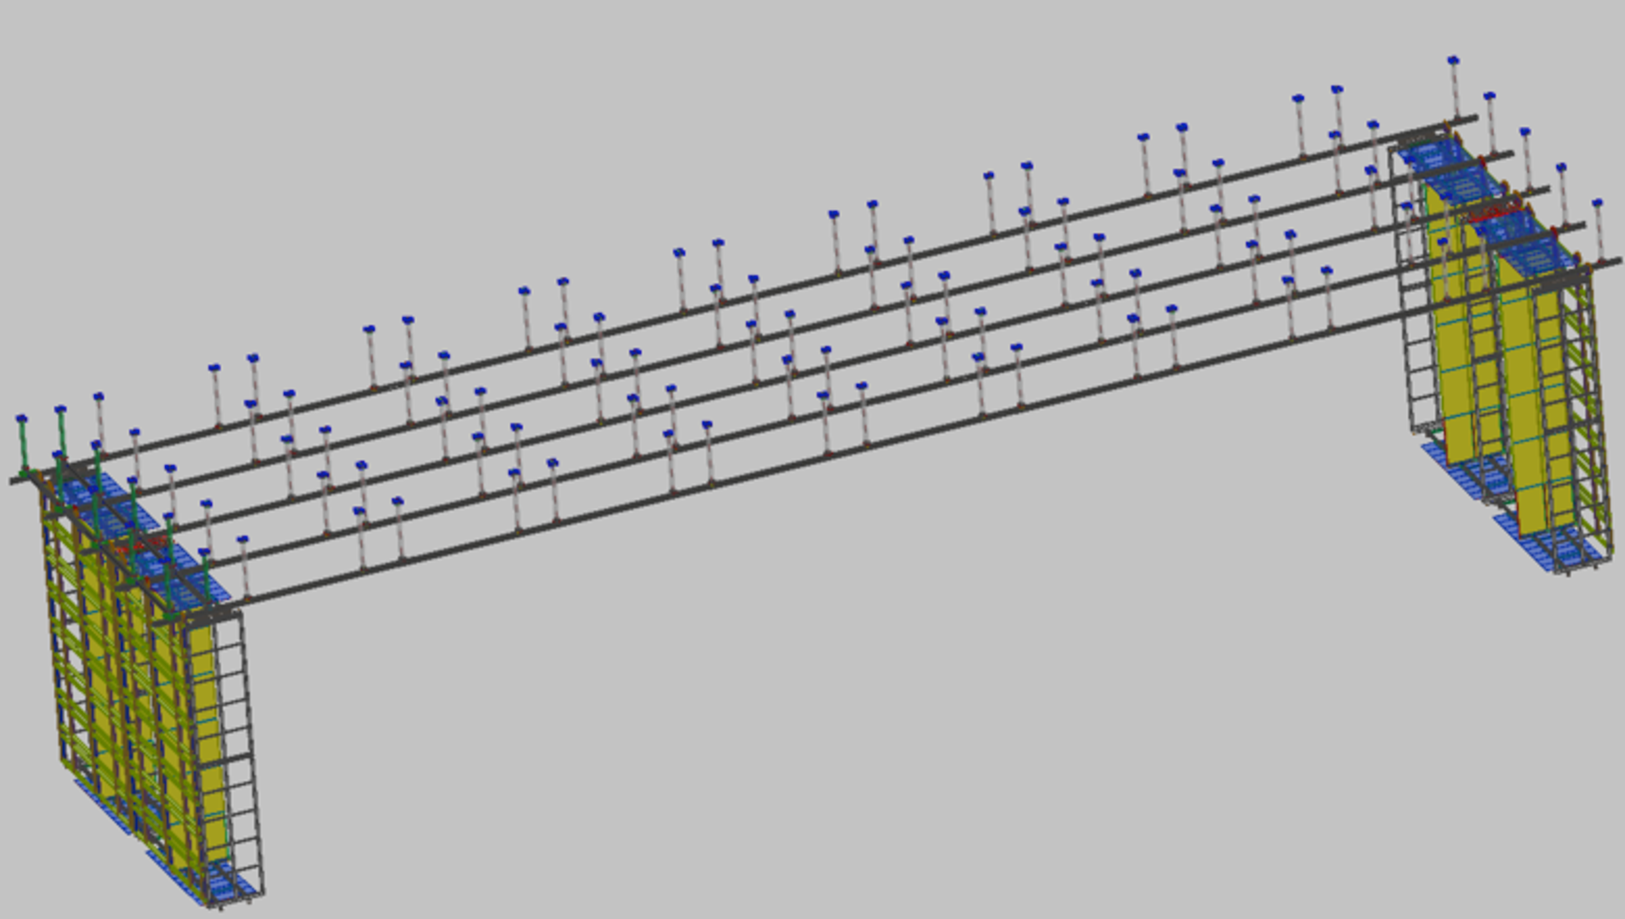
\includegraphics[width=.49\textwidth]{DSS-1.pdf}
 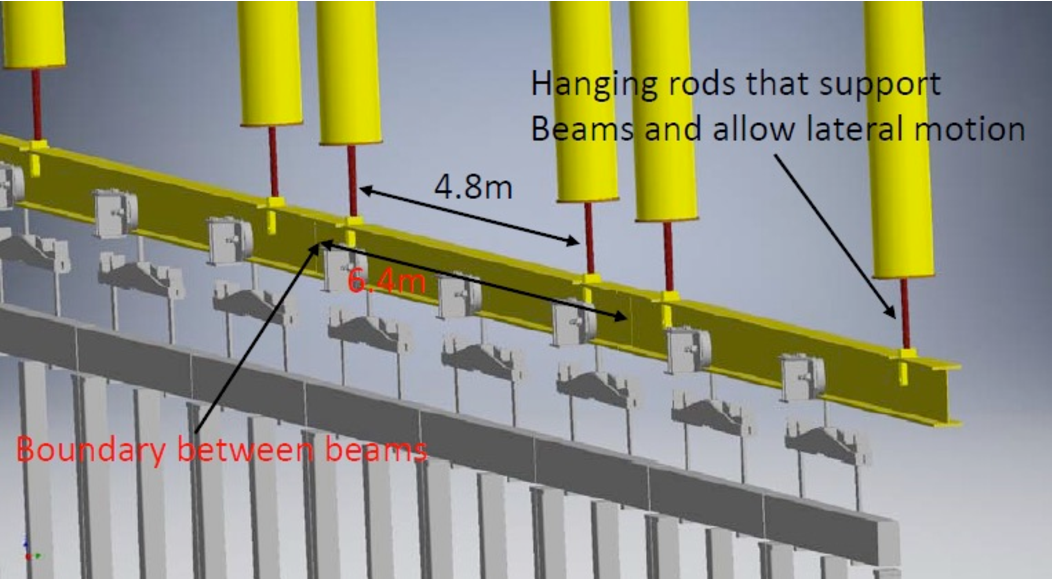
\includegraphics[width=.49\textwidth]{DSS-2.pdf}
\end{dunefigure}

The \dword{dss} is supported by the
cryostat outer steel structure through a series of \fdth{}s that cross through the cryostat insulation and anchored with flanges on
the cryostat roof. 
Inside the cryostat, a series of stainless steel I-beams are connected to the \fdth{}s and used to support the
detector. 
The \dword{dss} defines the location of the detector inside the cryostat and also defines how the detector elements move and contract as the detector is brought to \dword{lar} temperature. 
The design of the \dword{dss} encompasses the overall
structural design of the \dword{detmodule} because only after the elements are mounted to the \dword{dss} and connected do they make a unified mechanical structure. 
Figure~\ref{fig:DSS} (left) shows the \dword{dss} structure; there are
five rows of supports for the alternating rows of
\dword{apa}-\dword{cpa}-\dword{apa}-\dword{cpa}-\dword{apa}.  
The \dword{dss} is connected to the cryostat warm structure at a flange mounted on the outside of the cryostat.  
Figure~\ref{fig:DSS} (right)
shows the layout of these structural \fdth{}s.

The \dword{dss} is designed to meet the following  requirements:
\begin{itemize}
 \setlength\itemsep{1mm}
\setlength{\parsep}{1mm}
\setlength{\itemsep}{-5mm}
% \small
\item Support the weight of the detector;
\item Accommodate cryostat roof movement during filling, testing, and operation;
\item Accommodate variation in \fdth locations and
  variation in the flange angles due to installation tolerances and
  loading on the warm structure;
\item Accommodate shrinkage of the detector and \dword{dss} from ambient
  temperature to \dword{lar} temperature;
\item Define the positions of the detector components relative to each other; 
\item Provide electrical connection to the cryostat ground and remain electrically isolated from the detector;
\item Allow support penetrations to be purged with gaseous argon to prevent contaminants from diffusing back into the liquid; 
\item Ensure that the instrumentation cabling does not interfere with the \dword{dss};
\item Consist entirely of components that can  
be installed through the \dword{tco};
\item %Design to m
Meet AISC-360 or appropriate codes required at \dword{surf};
\item %Design to m
Meet seismic requirements one mile underground at \dword{surf};
\item Consist entirely of %All materials must be 
materials compatible for operation in ultrapure \dword{lar};
\item Ensure that beams are completely submerged in \dword{lar};
\item Ensure that detector components are not less than \SI{400}{mm} from the membrane flat surface;
\item Ensure that the supports do not interfere with the cryostat I-beam structures;
\item Ensure %Design such 
that the detector's lower \dword{gp} is lies over the cryogenic piping and that the tops of the \dword{dss} beams are submerged in \dword{lar} while leaving a \SI{4}{\%} ullage at the top of the cryostat;
\item Include the infrastructure necessary to move the \dword{apa} and
  \dword{cpa}-\dword{fc} assemblies from outside the cryostat through the
  \dword{tco} and to the correct position.
\end{itemize}

  The \dword{dss}
consists of pairs of \fdth{}s that support \SI{6.4}{m}-long
W10x26 stainless steel I-beam sections. The proposed design of the
\dword{dss} has \num{10} I-beam segments per row for a total of
\num{50} I-beam segments. Each I-beam is suspended on both ends by
rods from \fdth{}s that penetrate the cryostat roof.  %In the cold condition
When cold, each I-beam shrinks, causing gaps to form between
\dword{apa}s that are adjacent but supported on separate beams.
\dword{apa}s that are supported on the same beam will not have gaps
develop because both the beam and \dword{apa}s are stainless steel so
they shrink together.  Each beam is supported by a nearly
\SI{2}{m} long rod that allows the beam support to move as the beam
contracts.


The feedthrough consists of a flange and $6 ^{''}$ OD structural tube welded to it that extends through the cryostat insulation.  
There is a
nominal \SI{10}{mm} gap between the OD of the tube and the ID of the clearance tube in the cryostat. \fixme{OD and ID are not defined in the common glossary.}
The $6 ^{''}$ tube provides lateral support to the I-beams during installation.
Running down the center of the feedthrough is a $1^{"}$ diameter rod supported at a swivel washer at the flange and then supported by the
I-beam at a clevis.  The gas seal is obtained by Conflat Flange and a
bellows that seals around the swivel washer.  The lateral position and height of the rod can be adjusted $\pm$1 inch to accommodate tolerances in positioning cryostat crossing tubes. Figure \ref{fig:DSS-lateral-support} shows the end of the $6 ^{''}$ tube and how it locks the I-Beam into position. 

\begin{dunefigure}[DSS support for lateral loads ]{fig:DSS-lateral-support}
  {Left panel shows how the central support rod is locked in postion during detector installation. The outer $6 ^{''}$ tube is used to fix the support clevis in position. The right panel shows the system as it is connected to the I-Beam.}
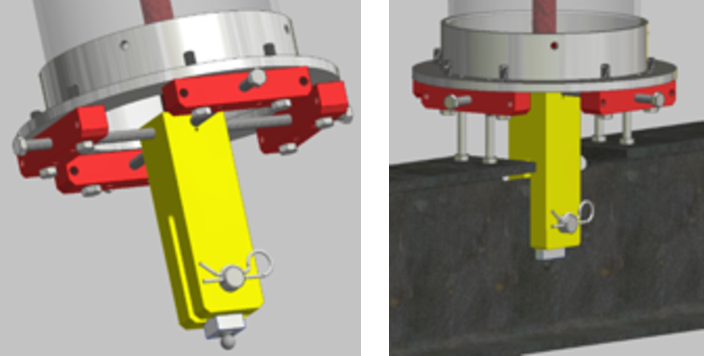
\includegraphics[width=.75\textwidth]{graphics/dss-lateral-support.pdf}
\end{dunefigure}

After the detector has been installed all restraints will be released to allow motion as the detector contracts during cool down.  The two hangars that support each \dword{dss} beam will contract and move toward each other by 13.1 mm along the axis of the detector.  
The drift distance will shrink by 7.4mm caused by the contraction of the field cages.  The detector is symmetric in the drift direction around the center \dword{apa}.  The drifts on either side of the center \dword{apa} will  shrink toward the center while the center \dword{apa} remains unmoved.  This results in the \dwords{cpa} moving 7.4mm toward the center and the outer \dword{apa}s moving 14.8mm (2*7.4mm) toward the center.  The hanging rod is designed to have a range of motion of 15mm in the drift direction to accommodate this shrinkage.




Detector components are installed using a shuttle beam system as
illustrated in Figure~\ref{fig:shuttle}.  
The last two columns of
\fdth{}s (eastern-most) support temporary beams that run
north-south, perpendicular to the main \dword{dss} beams.  
A shuttle beam has trolleys mounted to it and transverses 
north-south until it aligns with the required row of \dword{dss} beams.  
The last \dword{apa} or \dword{cpa} in a row is supported by the shuttle beam, which is bolted directly to the \fdth{}s once it is in place.  
As the last \dword{cpa} or \dword{apa} in each row is installed, the north-south beams are removed.

\begin{dunefigure}[\threed models of the shuttle beam end of the \dword{dss}]{fig:shuttle}
  {\threed models of the shuttle beam end of the \dword{dss}. The figures show how an \dword{apa}
is translated into position using the north-south beams until it lines up with the correct
row of I-beams.}
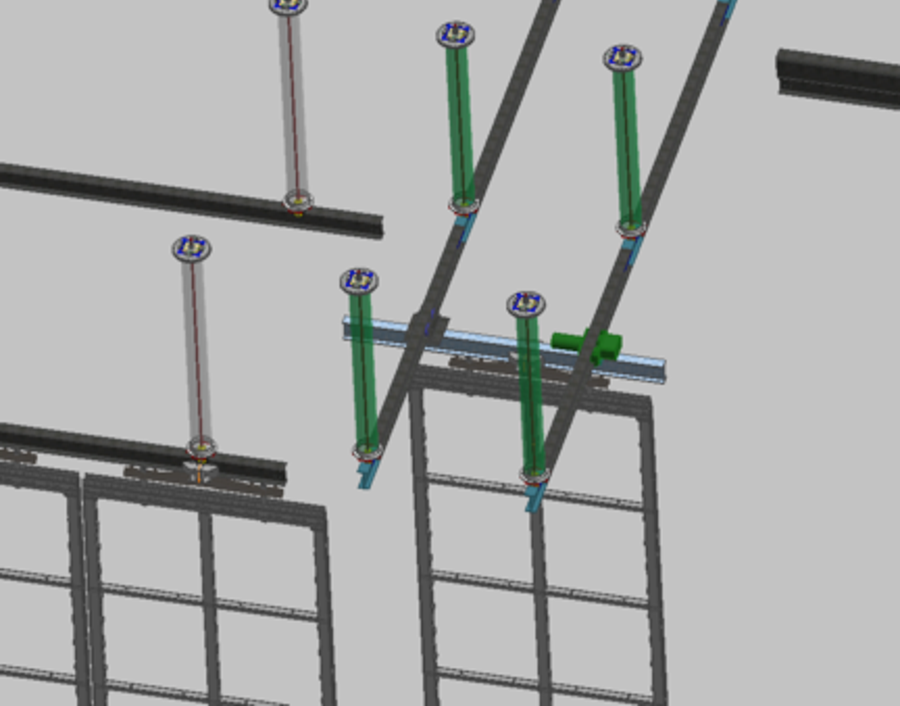
\includegraphics[width=.49\textwidth]{/Shuttle-1.pdf}
 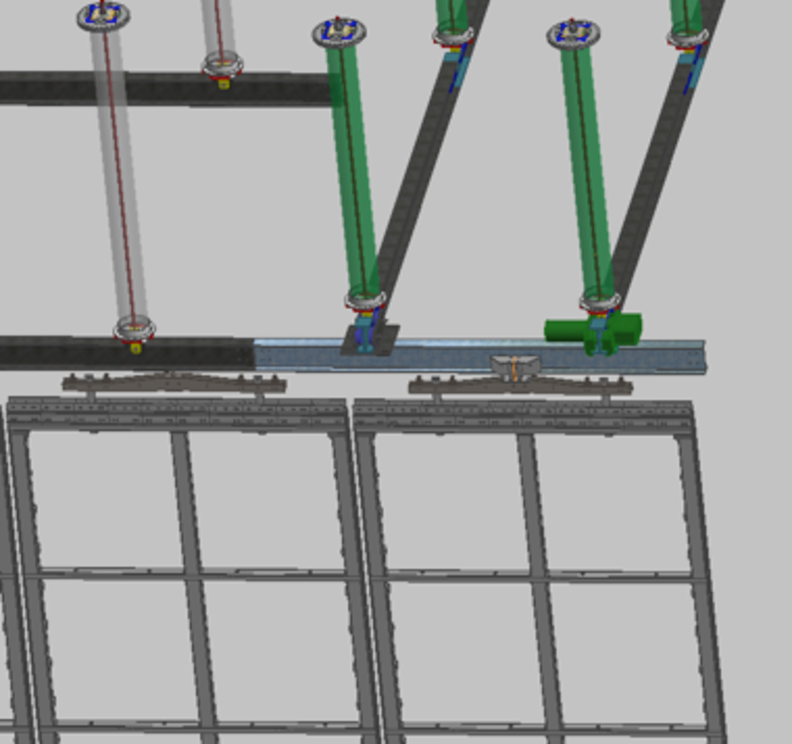
\includegraphics[width=.42\textwidth]{shuttle-2.pdf}
\end{dunefigure}

A mechanical interlock system  prevents trolleys
from passing the end of the shuttle beam unless it is aligned with a
corresponding \dword{dss} beam.  The shuttle beam and each detector component are
moved using a motorized trolley.  A commercially available motorized
trolley will be modified as needed for the
installation. 




\begin{dunefigure}[Prototype of the motorized DSS trolley ]{fig:DSS-trolley}
  {Prototype of the motorized DSS trolley that will push the APA and CPA along the I-beams and through the switchyard.}
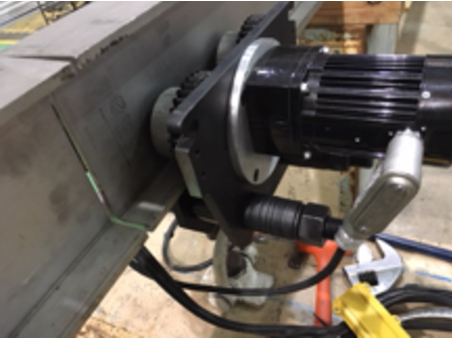
\includegraphics[width=.49\textwidth]{graphics/DSS-trolley.pdf}
\end{dunefigure}



A mock-up of the shuttle system will be constructed to test the
mechanical interlock and drive systems for the shuttle beam
for each \dword{detmodule}.  Tests will be conducted to evaluate the level of
misalignment between beams that can be tolerated and the amount of
positional control that can be achieved with the motorized trolley. We plan to construct a full scale prototype of a section of the  switchyard and perform tests at floor level. Later, the test program will be expanded at Ash River, where a full scale installation test will be performed. This is described in the installation \dword{qa} section.


%%%%%%%%%%%%%%%%%%%%%%%%%%%%
\subsection{Cryostat Roof Infrastructure}
\label{sec:fdsp-tc-infr-cryo-roof}

\begin{dunefigure}[Mezzanine and electronics racks]{fig:mezzanine}
  {The electronics racks sit on the \dword{dune} electronics mezzanine as shown. The top image is a view from above the detector looking at the racks from the side. In this view the cavern and cryogenics mezzanine are hidden. The bottom view is from the end of the cryostat looking over the roof. Here, the access stairs to the mezzanine are shown.}
 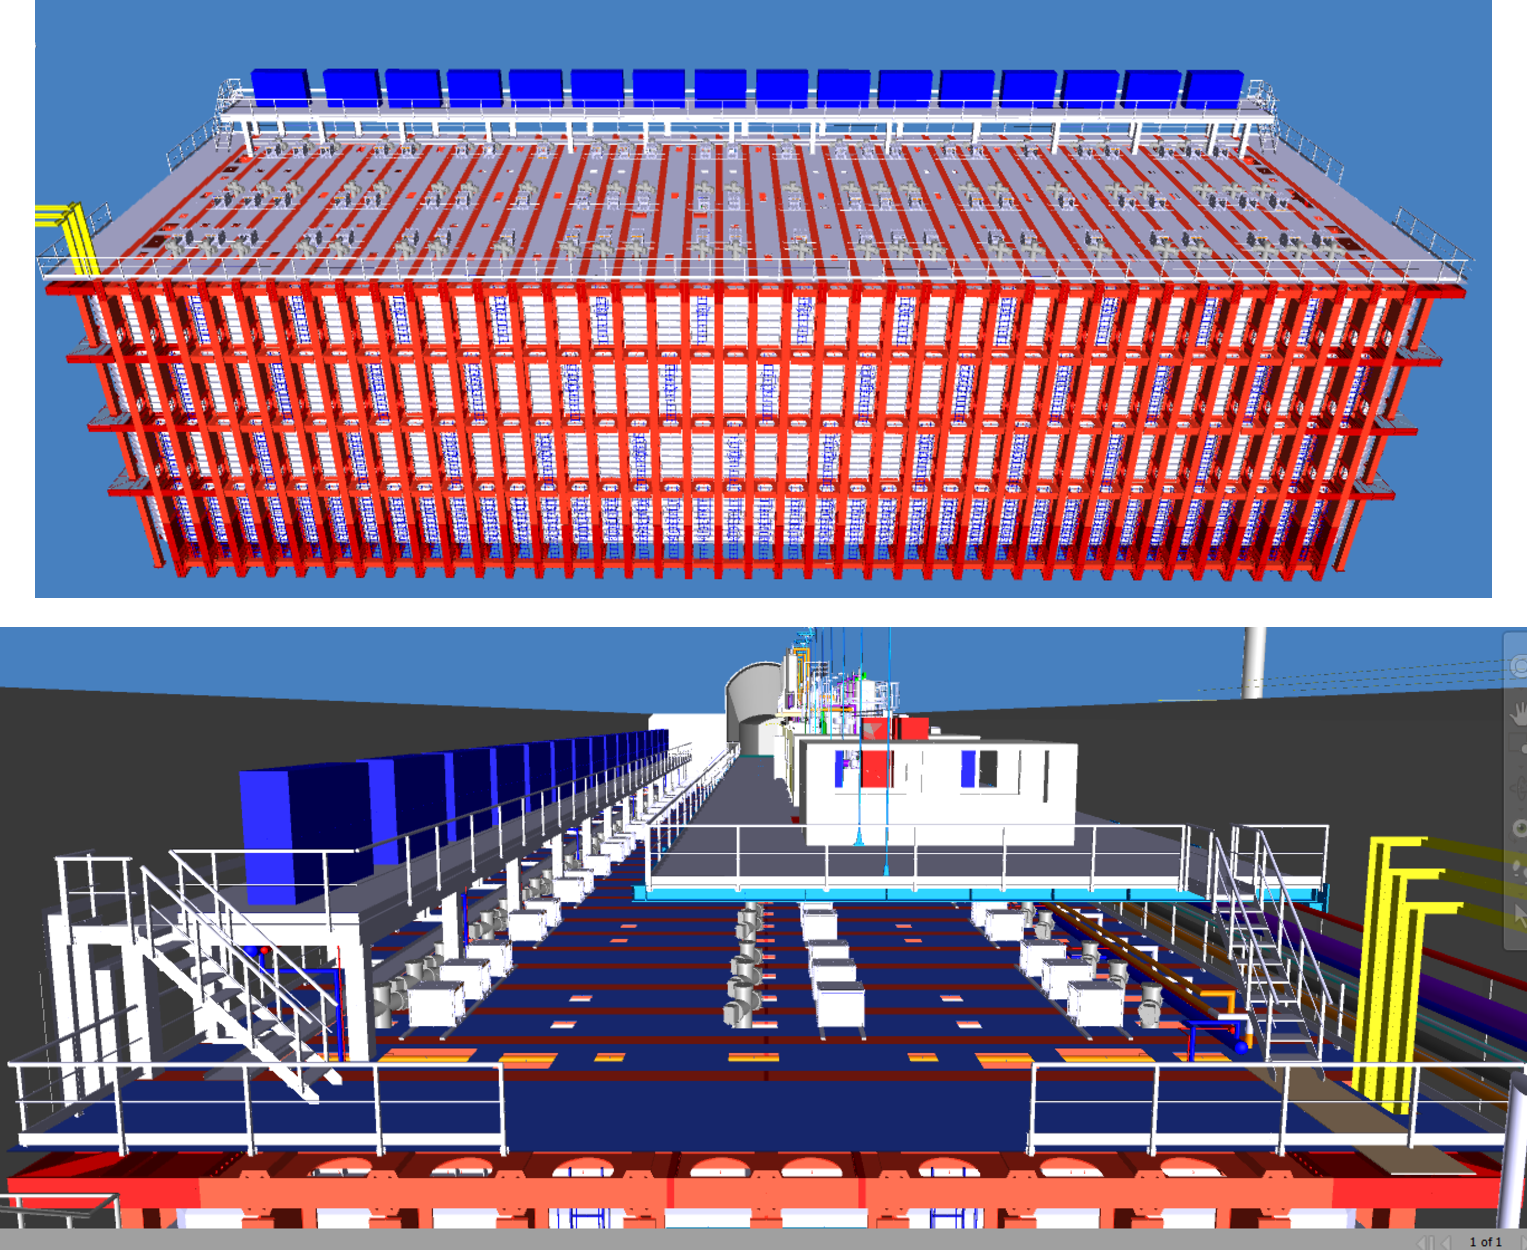
\includegraphics[width=\textwidth]{mezzanine.pdf}
\end{dunefigure}

\begin{dunefigure}[Electronics rack contents]{fig:rack-build1}
  {The nominal contents of the electronics racks on the mezzanine is shown. Each rack is configured to consume less than 3.5 \si{kW}. \fixme{Weiner is miss-spelled in the table should be Wiener}}
 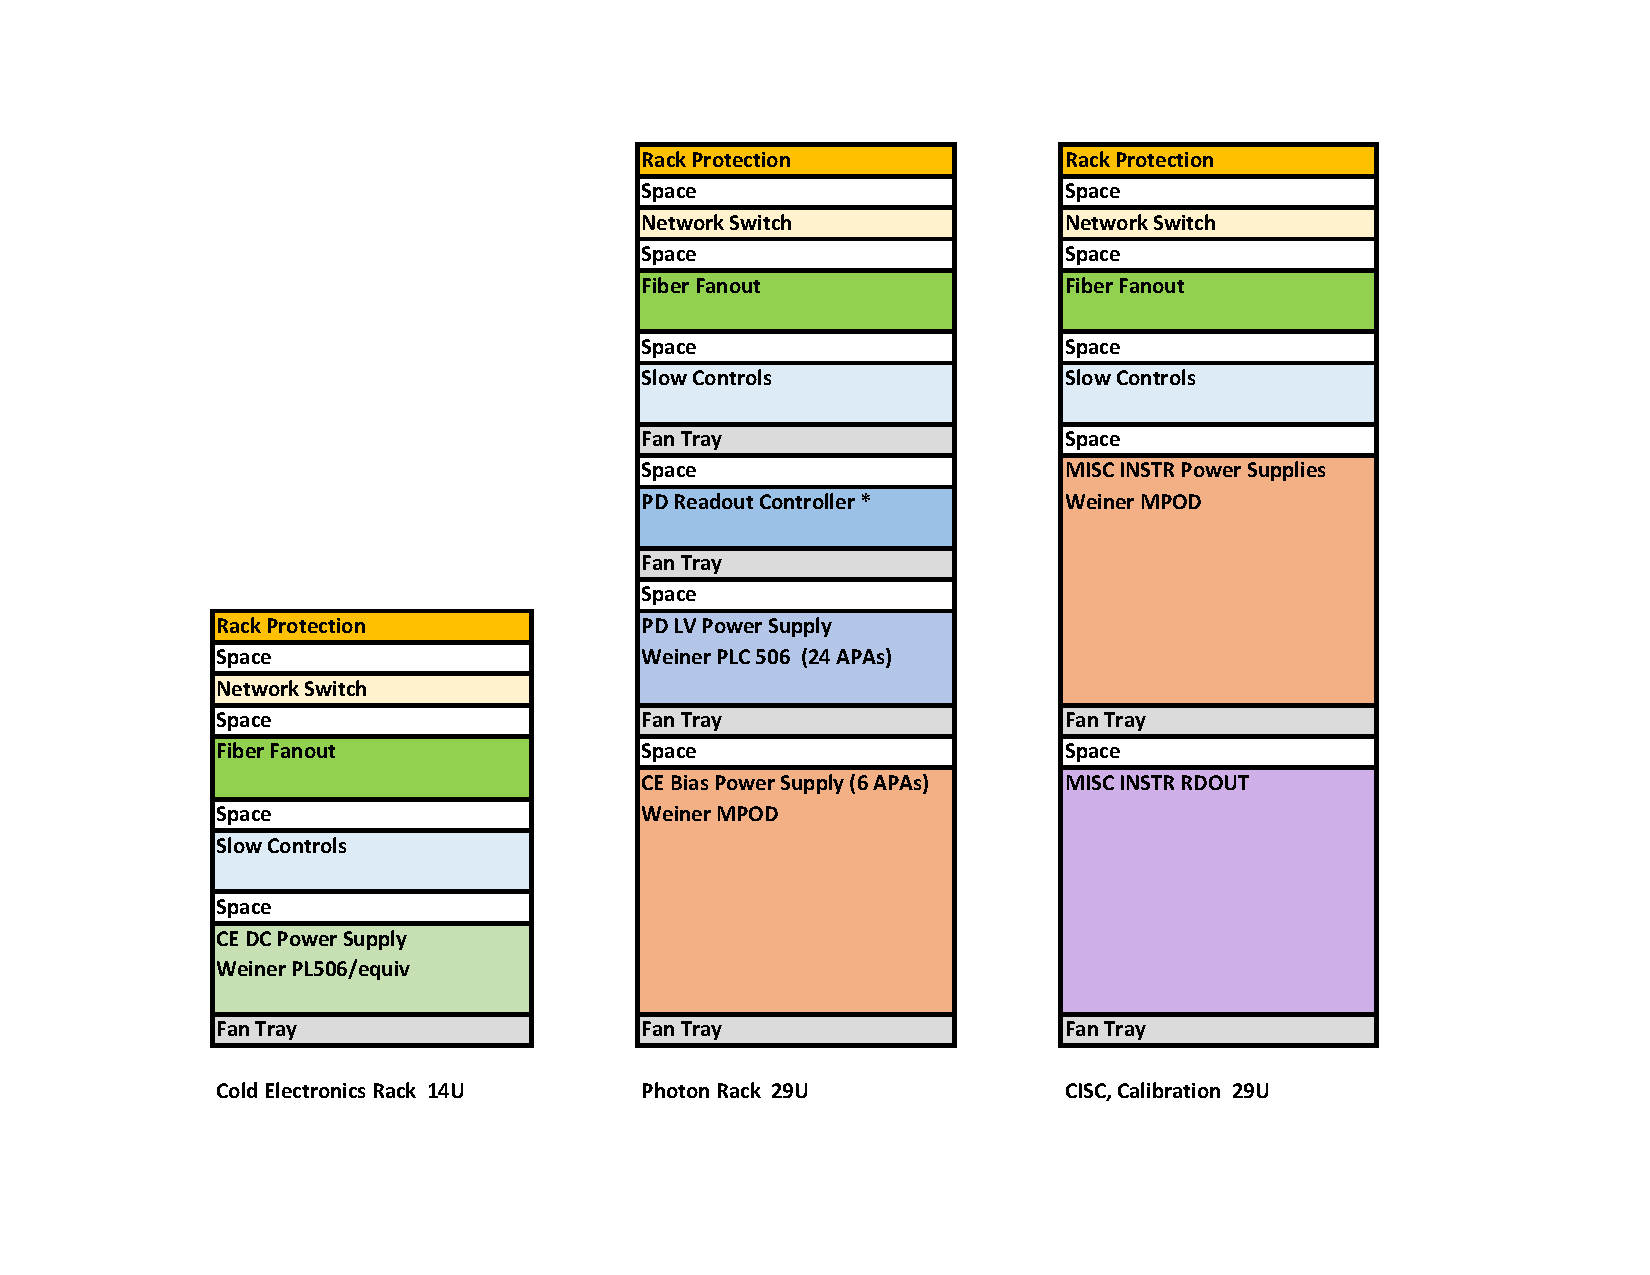
\includegraphics[width=.8\textwidth]{rack-build1} 
\end{dunefigure}

The top image in Figure \ref{fig:mezzanine} shows the \dword{dune} electronics mezzanine with the 42U tall racks placed on top. 
During the initial design steps, it became clear that the constraints placed on the rack location by the many \dword{dss} support \fdth{}s, the electronics \fdth, and the I-beams themselves make distributing the racks on the roof very challenging. 
By constructing a fixed mezzanine for the electronics above the cryostat at the same height as the cryogenic mezzanine, the electronics \fdth{}s are kept clear. 
This configuration also makes working on the electronics much easier because there are no local obstacles and all the racks are in one place.

As the electronics modules in the  racks are connected to the detector readout electronics they are by definition at detector ground so the mezzanine must also be connected to detector ground, which is accomplished by bolting the mezzanine to the cryostat I-beams. 
 \fixme{need input from Terri}
 
Figure \ref{fig:mezzanine} (top) shows 16 groups of five racks each
on the mezzanine for a total of 80 racks. 
The electronics inside the detector racks will be air cooled and the heat rejected into the cavern air. 
If the cavern temperature increases beyond an acceptable level due to the electrical heating then water cooled heat exchangers can be added to the racks. \dword{cf} will provide sufficient chilled water capacity at the entrance to the north cavern to accommodate the maximum heat load. 
The major heat load resides with the cold electronics and photon electronics located near the cryostat \fdth{}s which is difficult to water cool. 
The cooling capacity of the cavern air conditioning system roughly matches the expected heat generation by the electronics modules for one detector so it is not expected to need the additional chilled water capacity until detector \#3 is installed. 
At this time either the racks can be switched to chilled water cooling or the chilled water can be used for an additional air handling unit in the cavern.


Of the 80 racks, \dword{ce} \dword{lv} power require \num{25}, and another 25 will be made available collectively for  \dword{apa} wire bias voltage, \dword{pd} power and miscellaneous additional \dword{ce}, \dword{pds}, and  \dword{apa} electronics modules. 
The remaining 30 will be available for slow control, calibration, and other electrical equipment. 
Small 12U high mini-racks will  be placed near the electronics \fdth{}s for the \dword{pd} readout electronics and optical patch panels. If this is not enough, additional racks can be placed on the cryostat roof. The present rack configuration for this layout is shown in Figure~\ref{fig:rack-build1}. 
The electronics modules inside the racks are distributed to keep power consumption for each rack below \SI{3.5}{kW}. 
The racks are 42U high, which provides significant extra rack space.  
\fixme{reference docdb 4499 "Working document exploring Rack Requirements and layout" T. Shaw}


The 12U high mini-racks near the \fdth flanges will be relatively empty because the \dword{pd} readout should need only approximately 2U in height while the \dword{ce} patch panel needs less than 1 U. The mini-racks are shown in the lower panel of Figure \ref{fig:mezzanine}; 
they are the gray rectangles near the electronics crosses.

The north-south cable trays (transverse to the beam) which run from the electronics mezzanine to the electronics \fdth are routed under the floor of the cryostat roof (shown in gray in Figure \ref{fig:mezzanine}) next to the 
I-beams. 
This keeps the roof reasonably clear, so that equipment can be transported across it.
The gap between the web of the I-beams is \SI{1.2}{m} so 
a \SIrange{200}{300}{mm} wide cable tray installed along the beams 
leaves enough space for people to work on the electronics crates while standing directly on the cryostat's outer steel skin (Figure \ref{fig:install-elect-cross}). 
The cable trays between the \dword{cuc} and the electronics mezzanine will run along the west end of the cryostat under the floor of the cryostat roof. 
We estimate only half of the \SI{1.6}{m} space is needed, so the cable tray quantity could in principal be doubled if necessary. 

The flooring material for the \dword{spmod}
will be similar to the \SI{25}{mm} thick plywood used at \dword{pdsp}. 
It must be easy to cut so as to fit around many obstacles and pipes on the roof, it must be light enough to lift up to allow access under the floor, and it must support the load of a person and a small cart. 
We will investigate fire-retardant options available in the USA, with input from the \dword{fnal} fire life-safety group. 

Air filters for the cleanroom and inside the cryostat will also be placed on the cryostat roof. The present plan is to place fan filter units near the manholes on the east end of the cryostat. Initial calculations indicate sufficient airflow is possible to support one air exchange per hour inside the cryostat. The air handling system has yet to be designed in detail.


\begin{dunefigure}[Cryostat crossing tube design]{fig:crossingtube}
  {Draft drawing of the cryostat crossing tubes. The hatched region is the cryostat insulation. Units are mm. Points labeled ``u'' and ``v'' are welds. }
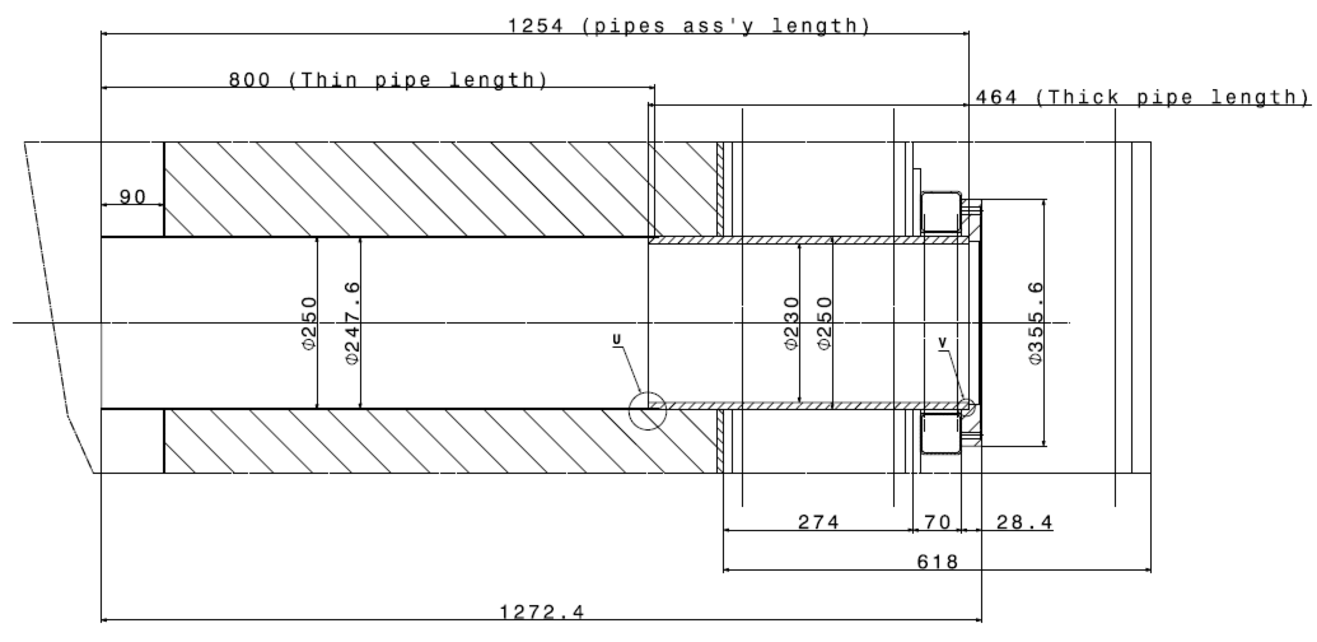
\includegraphics[width=.85\textwidth]{crossingtube}
\end{dunefigure}
 
The cryostat crossing tubes are among the most critical components of the roof infrastructure since they penetrate the cryostat roof and connect to the cold cryostat membrane. The top flange of the crossing tube supports either the electronics \fdth or the detector support \fdth and must be directly tied to the steel I-beams for support. 
Accurate placement and true vertical installation of the crossing tubes is important to ensure proper interfacing to the cryostat membrane. 
A draft assembly drawing of the crossing tube is shown in Figure~\ref{fig:crossingtube}. 
The crossing tube consists of a \SI{464}{mm} long stainless steel pipe with a \SI{1}{cm} thick wall. 
One end of the thick walled section is welded to a \SI{800}{mm} long \SI{250}{mm} diameter thin walled tube which is also welded to the cryostat membrane.
A custom Conflat flanges at the top end of the crossing tube connects to the \fdth. 
The thick tube section is also welded to the steel roof plates (the thin cross-hatched segments in Figure~\ref{fig:crossingtube}).  


%To ensure that the crossing tubes are adequately cleaned during the initial gaseous argon (\dword{gar}) purge and that air is removed from the tubes, each crossing tube has a small side port connected to a network of pipes on the roof of the cryostat. During the initial \dword{gar} purge, argon gas is withdrawn from each port and analyzed to assess progress and determine when the system is ready to be cooled down. The large number of crossing tubes, about 250 in the \dword{sp} configuration, means the content from each port cannot be analyzed independently of all others. Five streams, each one collecting gas from about 50 crossing tubes are connected independently to the gas analyzers. Gas impurities accumulate in the ullage. During steady state operations, \dword{gar} from the crossing tubes will be analyzed to ensure that impurities are adequately removed from the \dword{gar}.    If additional cleaning of the ullage is necessary, the \dword{gar} withdrawn from all ports, or a smaller set of them, can be sent to the condenser, re-condensed, and purified in the liquid phase along with the rest of the \dword{lar}. To detect any possible leaks that could develop in the room temperature feedthroughs over time, simple O$^2$\ sensors monitor the return gas for traces of oxygen, which would indicate a leak.
 
Each or the 250 crossing tubes has a small side port which connects to the cryogenic gas handling system through a network of pipes on the cryostat roof. During the initial \dword{gar} purge,  \dword{gar} is withdrawn from each port and analyzed to assess progress and determine when the system is ready to be cooled down. Five \dword{gar} streams, each collecting gas from 50 crossing tubes, are connected independently to the gas analyzers. This provides some redundancy and position dependant information on the contamination level of the gas a the top of the cryostat during the purge.
 
During filling and normal operation the collection and analysis of the gas from the crossing tubes will continue to ensure that impurities, which are generated in the cables in the \fdth{}s or the warmer surfaces in the ullage,  are adequately removed from the \dword{gar}. If the gas analyzers find no significant nitrogen contamination, the \dword{gar} from all or a subset of ports can be sent to the condenser, re-condensed, and purified along with the rest of the \dword{lar}. Simple O$_2$\ sensors monitor the return gas for traces of oxygen, which would indicate development of a leak in the room temperature \fdth{}s.

Each detector has a power budget of \SI{500}{kVA}. The total power budget available for use by detector electronics is derated to \SI{400}{kW} at the power distribution panels.  The \dword{ce} is the detector's largest power consumer.  
The \dword{ce} dissipates \SI{306}{W} per \dword{apa}.  
The \dword{lv} power supplies' controller needs about \SI{35}{W} per \dword{apa} and has an efficiency of approximately 85 percent. This leads to an approximately  \SI{400}{W} load per \dword{apa}, or a total load of  \SI{60}{kW} per \dword{detmodule}.  The \dword{apa} wire-bias power supplies have a maximum load of  \SI{465}{W} per set of six \dword{apa}s, for a total budget of around  \SI{12}{kW}.   Cooling fans and heaters near the \fdth{}s will use a nominal amount of power, so the overall power budget for \dword{ce} and  \dword{apa}
is expect to be less than \SI{75}{kW}.


The \dword{pds} electronics is based on the Mu2e electronics, which reports a power load of approximately  \SI{6}{kW}.  \dword{dune} plans a power budget of  \SI{8}{kW} because of cable drops and  power supply inefficiencies.  

Each of the approximately 80 detector racks will have fan units, Ethernet switches, rack protection, and slow controls modules, adding a load of about \SI{500}{W} per rack, for a total of \SI{40}{kW}.

Twenty-five racks are reserved for cryogenics instrumentation with a per-rack load conservatively estimated at \SI{2}{kW}, for a total of \SI{50}{kW}. 

The \dword{detmodule} will thus use  an estimated \SI{173}{kW} of power.   These numbers provide a safety factor of about two on our power estimates relative to available power.


%%%%%%%%%%%%%%%%%%%%%%%%%%%%
\subsection{Cryostat Internal Infrastructure}
\label{sec:fdsp-tc-infr-cryo-int}

%%%%Internal Cryogenics%%%%
\label{sec:fdsp-tc-internal-cryo}

The internal cryogenics comprises three sets of pipe distribution networks and two sets of sprayers. All pipes enter the cryostat from the top; some go all the way down to the floor, and others remain in the ceiling. On the floor are
\begin{itemize}
\setlength\itemsep{1mm}
\setlength{\parsep}{1mm}
\setlength{\itemsep}{-5mm}
\item \textbf{GAr distribution}: a set of pipes flowing GAr. These pipes are used only at the beginning to remove air that fills the cryostat. They have either a longitudinal slit or calibrated holes to distribute GAr uniformly along the length of the cryostat. Computational fluid dynamics simulations show that air will be removed from the system as long as GAr is flowing in at the right speed, calculated and experimentally verified as \SI{1.2}{m/hr}.


\item \textbf{\dword{lar} distribution}: two sets of pipes flowing \dword{lar}. These pipes are used to fill the cryostat and, during steady state operations, to return the \dword{lar} from the purification system. The pipes have calibrated holes to return the \dword{lar} uniformly throughout the length of the cryostat. This is very important for uniform purity. Four pumps circulate the \dword{lar}. Initially, all of pumps operate at once to achieve purity, but once the target purity is achieved, only one or two pumps remain in service. Two sets of pipes are needed to adequately distribute the \dword{lar} over this broad range of flow rates.
\end{itemize}

On the ceiling are

\begin{itemize}
\setlength\itemsep{1mm}
\setlength{\parsep}{1mm}
\setlength{\itemsep}{-5mm}
\item \textbf{Cool down sprayers}: Two sets of cool down sprayers are distributed along the long sides of each cryostat. One set distributes \dword{lar} using liquid sprayers that generate a conical profile of small droplets of liquid. The other set of sprayers distributes GAr to move the \dword{lar} droplets inside and cool down the detector and cryostat uniformly. These sprayers are being tested in \dword{pddp}. They are a variation of those implemented in \dword{pdsp}.
\end{itemize}

Figure~\ref{fig:internal-cryo-3D} shows the current layout of the internal cryogenics. 
%The current drawing of the internal cryogenics is presented in Figure~\ref{fig:internal-cryo-drawing}. 
The GAr pipes are in red, the \dword{lar} pipes in blue.

\begin{dunefigure}[Cryogenic piping inside the cryostat ]{fig:internal-cryo-3D}
  {Layout of the internal cryogenics.}
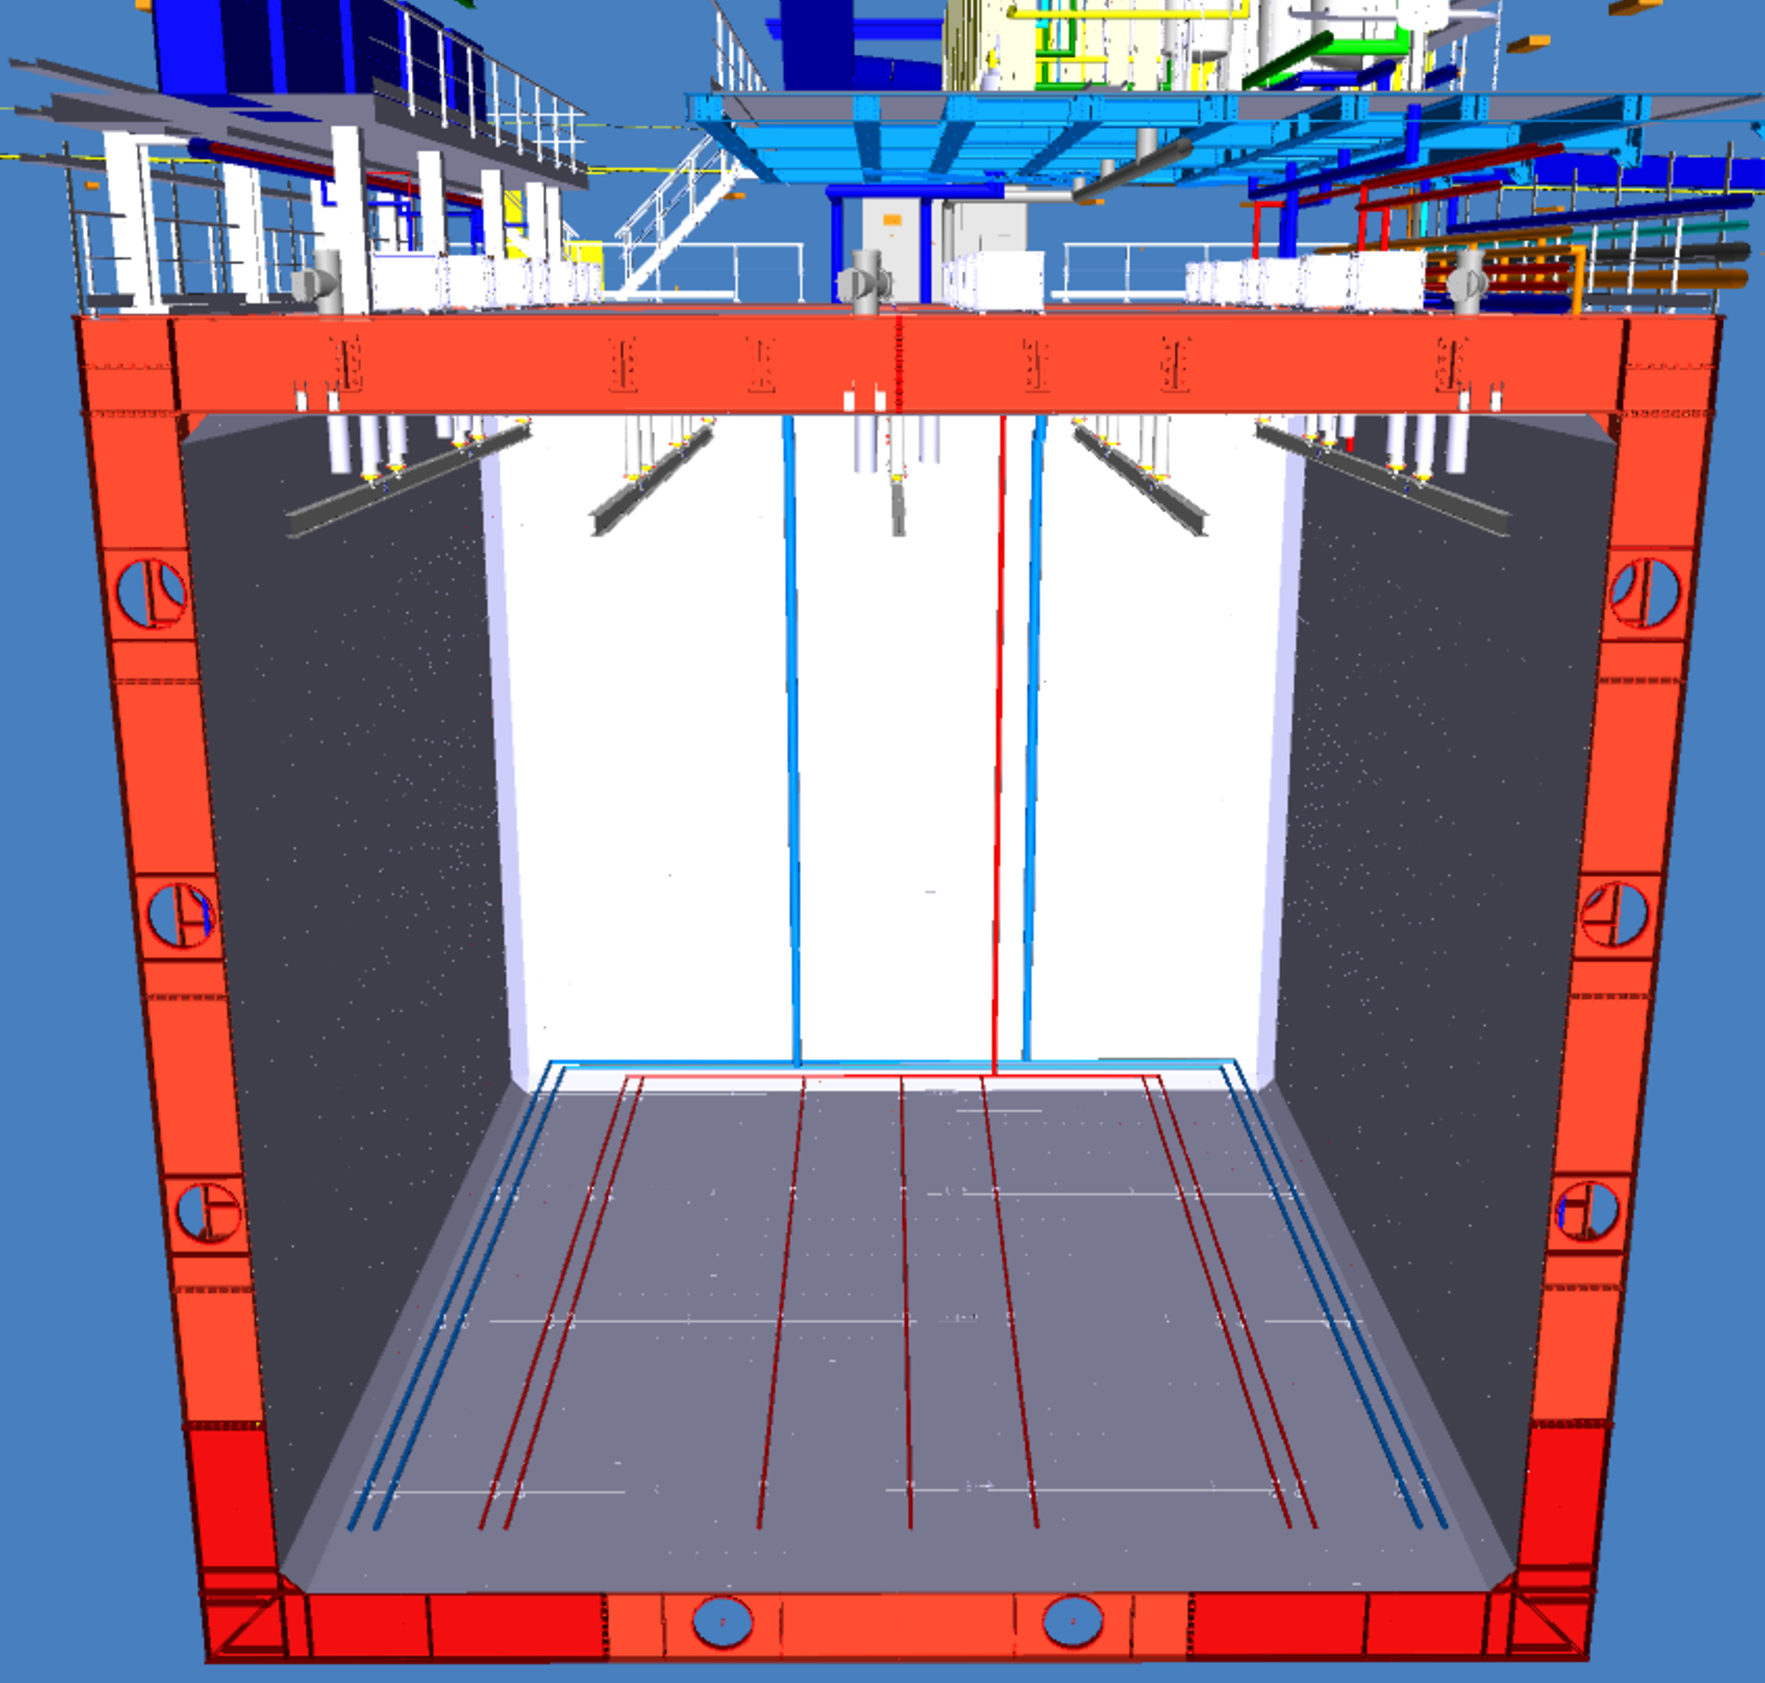
\includegraphics[width=.98\textwidth]{graphics/Internal-Piping-3D.pdf}
\end{dunefigure}

%\begin{dunefigure}[Drawing of the cryogenic %piping inside the cryostat %]{fig:internal-cryo-drawing}
%  {Drawing of the internal cryogenics.}
%\includegraphics[angle=90,width=.98\textwidth]{%graphics/Internal-pipes-HQ.pdf}
%\includegraphics[angle=90,height=.98\textheight%]{graphics/Internal-pipes-HQ.pdf}
%\end{dunefigure}
%\fixme{Please reduce size of Internal-pipes-HQ.pdf}


Other infrastructure inside the cryostat includes the cryostat false floor, the UV filtered lighting, and the battery-operated scissor lifts. 

The false floor requirements are not yet fully defined.  
It must support the load of the scissor lift used to work on the electronic cabling on the inside of the cryostat near the ceiling and allow the scissor lift to get close enough to the \dword{apa}s to work comfortably at the top. 
It  must be laid out so the panels can be removed in sections just before the equipment is installed. 
This is especially important for the \dword{apa}s where there is not enough room between the bottom of the \dword{apa}s and the floor to allow removal after installation. 

The cryostat lighting, using UV-filtered \dword{led} lamps, is expected to be fairly simple. Options for the lighting will be developed during the Ash River testing.
Floor-mounted lights with task lighting will be investigated. If needed, lighting can also be mounted to the \dword{dss} and removed as the detector is installed.

The plan is to use a commercially available battery-operated scissor lift with a \SI{12}{m} reach. Tests at Ash River will verify the stability of the lift at height. If the lift is determined to be suitable, then the remaining issue to resolve is how to install and remove it from the cryostat. 
The commercially available scissor lifts are too wide to fit through the \dword{tco} near the floor where the center post protrudes above floor level.
Custom lifting equipment will be needed to insert the lifts into the cryostat. 
At the end of the installation process, dismantling the last lift may be necessary to remove it from the cryostat.

% clear the figure buffer before starting the next section
%\clearpage

%%%%%%%%%%%%%%%%%%%%%%%%%%%%
\subsection{Cleanroom Infrastructure}
\label{sec:fdsp-tc-infr-comm}

\begin{dunefigure}[Installation Cleanroom layout]{fig:install-cleanroom}
  {Two views of the installation cleanroom.  The top view shows the cleanroom in position in the north cavern. The location of the material airlock and the changing room are indicated. The lower image is a closer view showing the equipment in the cleanroom. The cryostat is shown in red.
  } 
%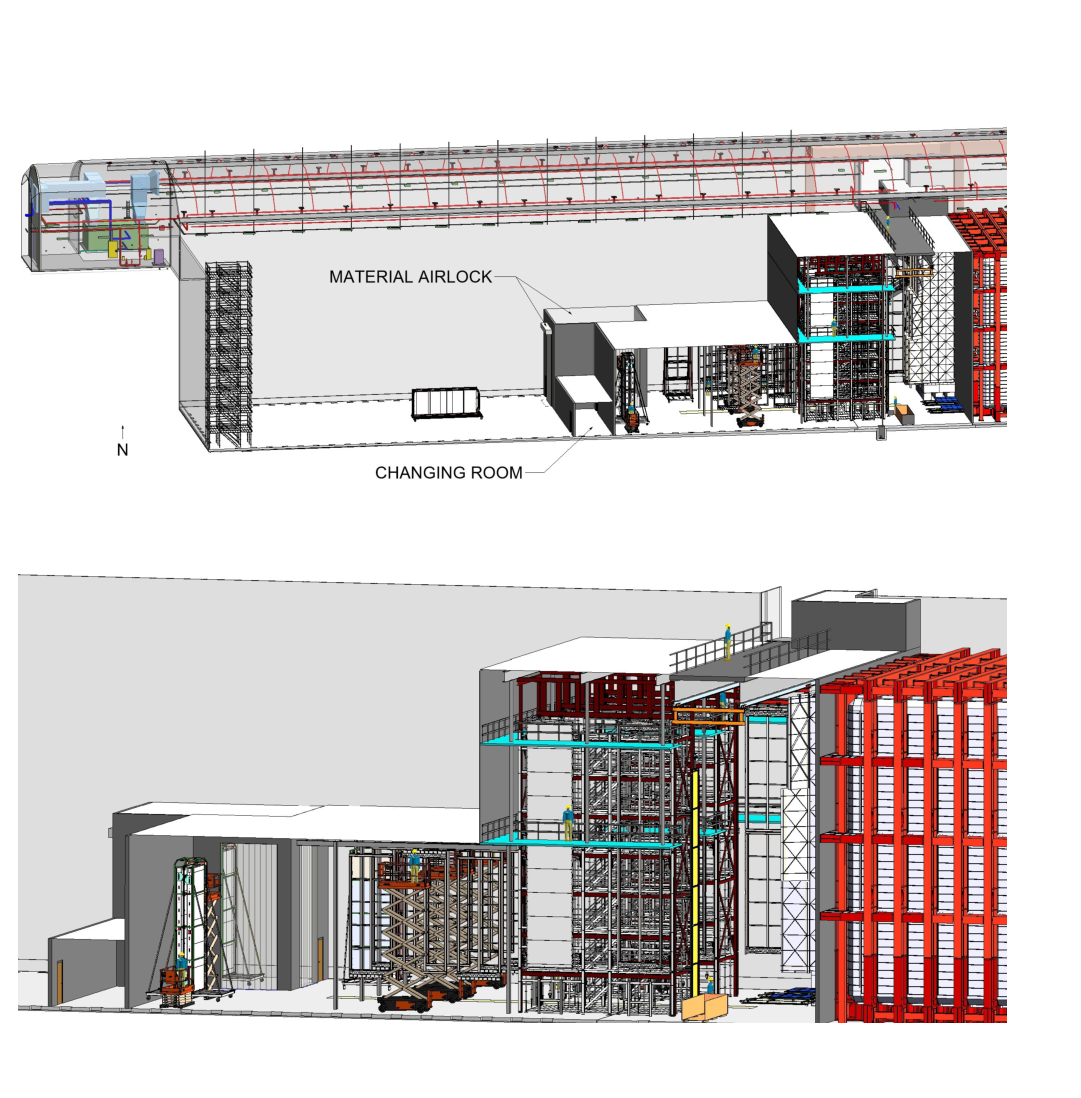
\includegraphics[width=1.0\textwidth]{graphics/install-cleanroom.pdf}
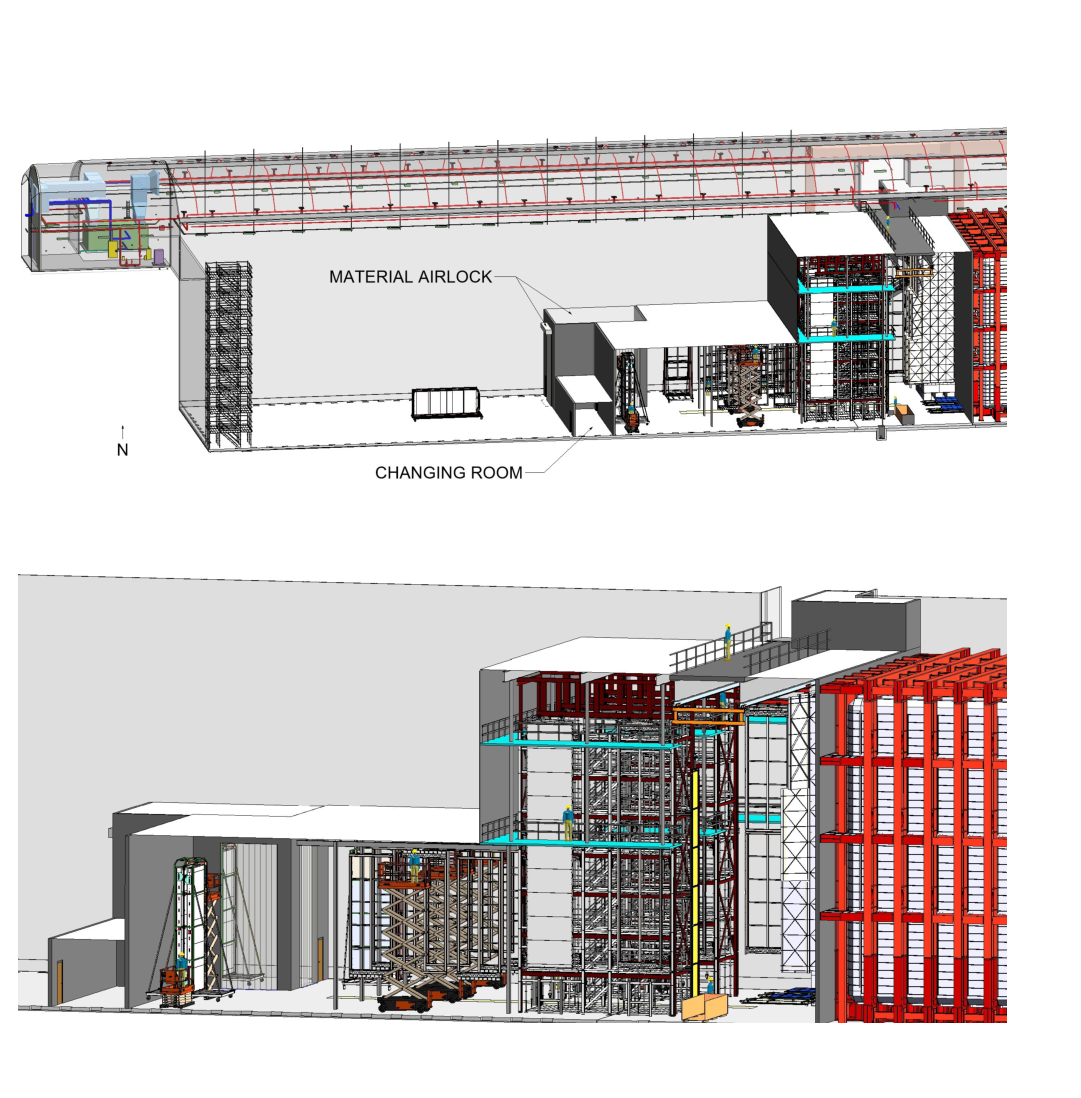
\includegraphics[width=1.0\textwidth]{graphics/install-cleanroom.pdf}
\end{dunefigure}

The cleanroom infrastructure consist of the cleanroom itself, the coldboxes and cryogenic plant for testing the assembled \dword{apa}, the assembly towers, rails and switchyard to allow the \dword{apa} to move inside the cleanroom, and the PD integration infrastructure. A combination of contractors and the lead worker and rigger teams will do the infrastructure work; they will also assist in detector assembly. 

The assembly of the detector sub-components into \SI{12}{m} tall full assemblies must be done underground directly outside the cryostat. 
The full assemblies are too large and fragile to be brought down the shaft, and the only place with enough vertical space to assemble them is in front of the cryostat itself. 
\dword{protodune} showed that it is critical to cryogenically test the completely assembled components immediately before installing them in the cryostat as this was the single step that found all the detector issues. 
The requirement that final assembly and testing be performed underground next to the cryostat implies that a suitable cleanroom be set up outside the cryostat. 
The cleanroom must meet the ISO-8 cleanroom standard to maintain the cleanliness of all the components entering the cryostat.  
Air will be filtered and then forced into the cryostat at the east end. The clean air will flow through the cryostat and out through the cleanroom and airlock. 
This will keep the inside of the cryostat at least at ISO-8.  
The airlock, cleanroom, and inside the cryostat will be outfitted with UV filtered lights to protect the photon detectors.

The dimensions of the cleanroom are determined by first planning the work performed inside. After the work flow is defined and the equipment needed has been sketched out the envelope of the work are can be established and the size of the cleanroom defined. Figure \ref{fig:install-cleanroom} illustrates  the conceptual design of the installation cleanroom. The top figure shows the cleanroom situated in the cavern next to the cryostat, the materials airlock and the changing room are on the west end. The bottom image is a closer view showing some of the equipment in the cleanroom. 



All the detector elements enter the cleanroom by passing through a materials airlock (Figure \ref{fig:install-cleanroom}). 
The material enter through large rollup doors that are sized to allow an \dword{apa} transport box (\SI{2.6}{m} by \SI{6.8}{m}) to enter in a vertical orientation. 
The airlock is \SI{7.5}{m} wide, \SI{5}{m} deep, and \SI{10}{m} tall while the rollup doors are \SI{3}{m} wide and \SI{7.5}{m} tall. 
It is expected the \dword{apa} box will be bolted to a custom pallet and moved with electric pallet jacks so door dimensions are sufficient. 
The changing room is 6 \si{m} wide and 7 \si{m} deep. 
The dimensions were chosen to allow 50 people to gown up for the cleanroom within a reasonable time. 
The requirements for work in an ISO-8 cleanroom are a cleanroom lab coat, clean shoes, and nets for hair and beards.  
This will be augmented with a clean hard hat and gloves for safety reasons. 



The cleanroom proper can be divided into several work areas as follows:
\begin{itemize}
\setlength\itemsep{1mm}
\setlength{\parsep}{1mm}
\setlength{\itemsep}{-5mm}
    \item Materials and Personnel airlocks,
    \item \dword{pd} integration area,
    \item Four \dword{apa} assembly lines where the lower rails are for wire tension measurements and the upper rails for APA  assembly and cabling,
    \item The switchyard area used to move the assembles APA in the cleanroom and into the cryostat,
    \item The \coldbox area where the APA are cold tested, and
    \item The HV assembly area.
\end{itemize}

\begin{comment}
The integration area at the west end of the cleanroom is where the \dword{pd} and \dword{ce}-\dword{femb} are integrated into the \dword{apa} and where the receiving quality assurance tests are performed. 
The activities are time consuming so three assembly lines are planned to keep up with the rate of installation in the cryostat. 
A fourth line is available for spare capacity and repair. 
The integration area measures \SI{19.5}{m} wide by \SI{21}{m} deep with a \SI{10}{m} ceiling, including the airlock area. 
A similar design is considered as what was used for the \dword{protodune} cleanroom as the height is similar. 
If needed the rail system inside the integration work area can be used to support the roof.
\end{comment}

The \dword{pd} integration area at the west end of the cleanroom is where the \dword{pd} are integrated into the \dword{apa} and where the initial receiving quality assurance tests are performed. 

Because the testing and assembly of the \dword{apa} into \SI{12}{m} tall doublets is time consuming the cleanroom has 4 assembly lines in order to keep up with the detector cold tests and installation. 
Three lines will be in continuous usage and the 4$^{\rm th}$ for repairs or contingency. 
Each assembly line has a lower and upper set of rails for moving the \dword{apa}.
The lower rails are where the wire tension is measured and the lower \dword{ce} \dword{femb} are installed. The \dword{pd} integration area and the lower rail section of the assembly lines measure \SI{19.5}{m} wide by \SI{21}{m} deep with a \SI{10}{m} ceiling, including the airlock area. 
A similar design is considered as what was used for the \dword{protodune} cleanroom as the height is similar. 
If needed the rail system inside the integration work area can be used to support the roof.
 
The \dword{apa} assembly and cabling area is where the top and bottom \dword{apa} are connected together to form a doublet and the \dword{ce} cables are inserted and connected to the \dword{femb}. 
This area has to be taller as the full \SI{12}{m} tall \dword{apa} doublets must be accommodated. 
The ceiling in this area is \SI{17.8}{m} placing the ceiling at the same level as the bridge and the roof of the cryostat. 
A \SI{9}{m} by \SI{19.5}{m} area is sufficient to house the two large assembly towers needed to support the assembly lines. Above the towers I-beams running north-south or transverse to the neutrino beam are needed to support work platforms which allow access to both faces of the \dword{apa}s these beams can be used to support the cleanroom roof which can be a light weight frame with a fire retardant fabric attached. 
The outer towers steel structure provides a strong surface to attach a polymer sheet serving as the vertical wall connecting the \SI{17.8}{m} region to the \SI{10}{m} tall area.

The switchyard area is the region under the north-south bridge where a bridge crane is mounted and is used to move the \dword{apa} from the assembly lines to the \coldbox{}es and into the cryostat. The \coldbox{}es and the HV assembly area are between the bridge and the cryostat.


The cleanroom is as wide as the cavern excavation. The side walls of the cleanroom will be consrtucted by hanging reinforced fire retardant plastic sheets against the wall. This will result in a low cost construction that is easy to install.


\begin{dunefigure}[Installation Integration Lower Rail System]{fig:install-integrate-rail}
  {Two pairs of rails are used to prepare the \dword{apa} for assembly. Each rail will hold three \dword{apa}. Here the wire tension measurements are performed and the \dword{ce} \dword{femb} are installed on the lower \dword{apa}. The lower \dword{ce} are easily reachable from the floor in this arrangement. This view is from the assembly towers looking west along the assembly lines.}
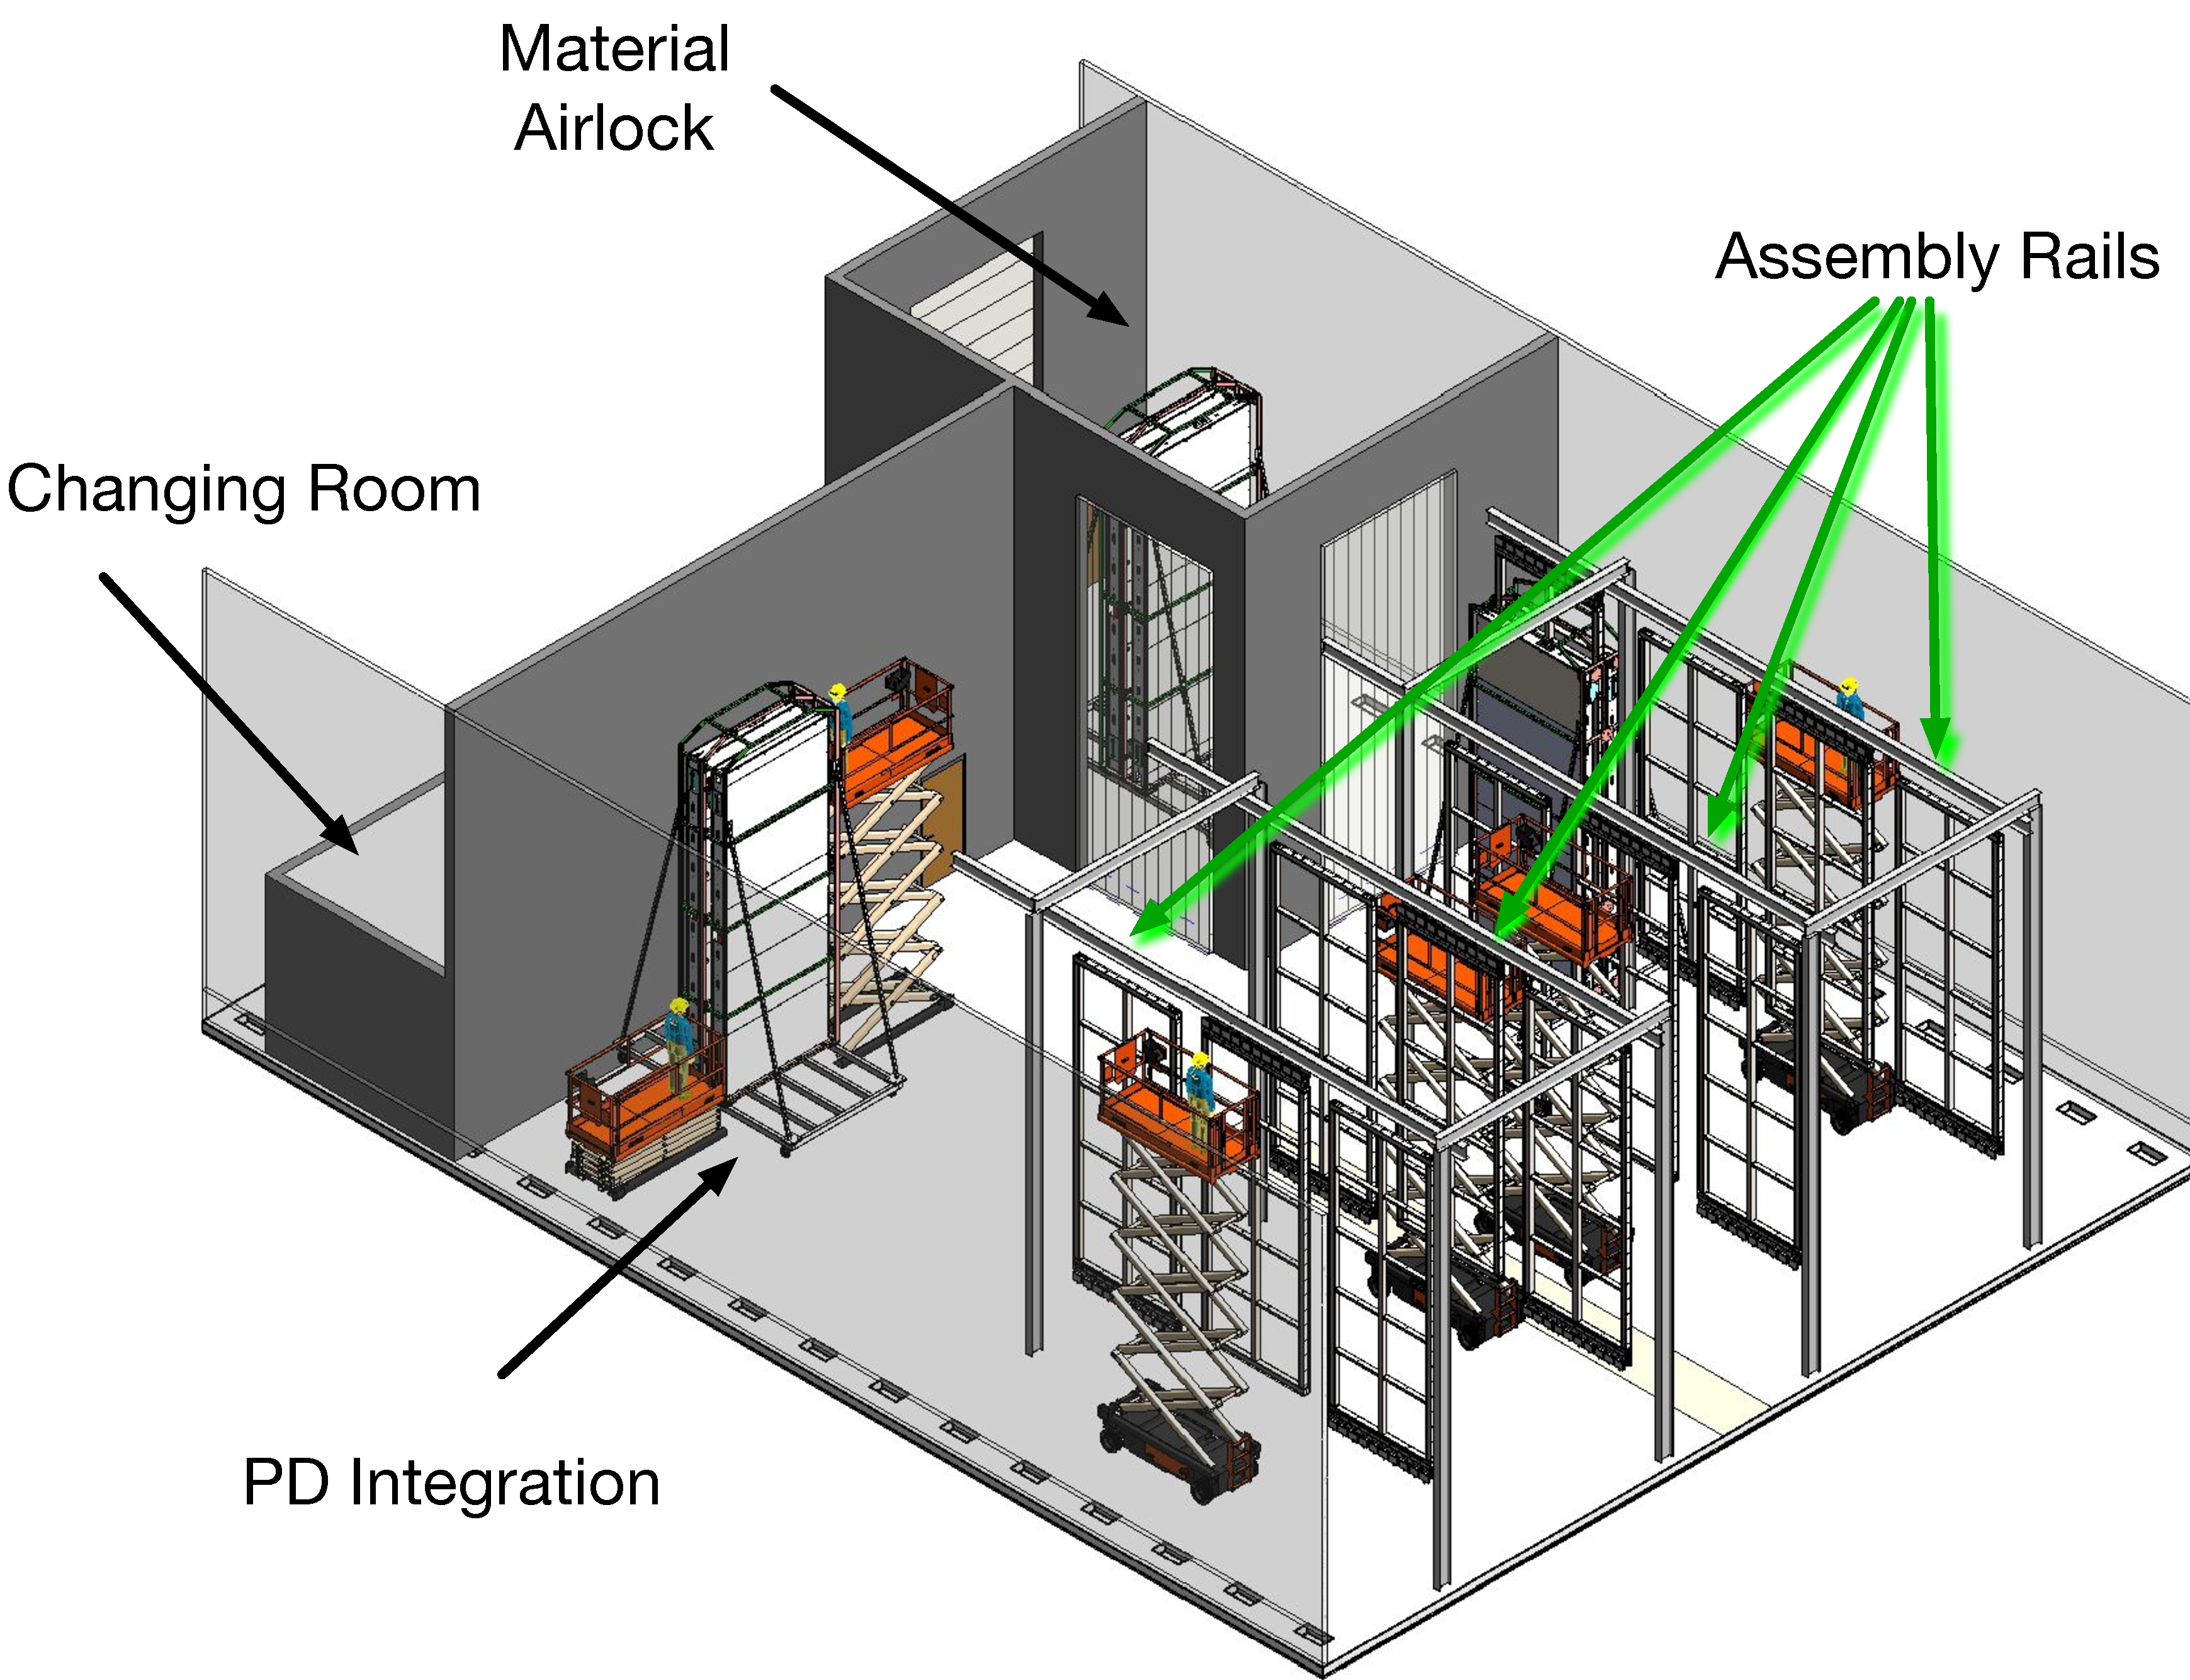
\includegraphics[width=.6\textwidth]{graphics/install-integrate-rail.pdf}
\end{dunefigure}

Given the substantial size and the significant occupancy, the cleanroom will have electrical outlets, UV filtered lighting, and fire protection.

Equipment in the integration work area will consist of a station for integrating the photon detectors into the \dword{apa} and two pairs of rails for preparing the \dword{apa} for assembly and several scissor lifts for working around the \dword{apa}. 
The area adjacent to the materials airlock is reserved for integration the \dword{pd} into the \dword{apa}. 
The \dword{apa} transport box will be positioned between two fixed lifts. 
The lifts are raised until the photon detector paddles can easily be inserted into the side of the \dword{apa}.
Figure \ref{fig:install-integrate-rail} illustrates the rail setup in the integration work area. 
The \dword{apa} are removed from the transport box and mounted to the rails at the far end. 
They then move along the rails using simple trolleys running on the I-beams. 
The rails are long enough to hold three \dword{apa} at a time. 
This setup is conceptual and engineering design of the rail supports has not yet started. 
Cross bracing of the vertical posts will be added during the design stage. 

\begin{dunefigure}[APA cabling tower]{fig:install-assembly-tower}
  {
  Isomtetric view of the \dword{apa} assembly and cabling tower. 
  The tower is designed to be two \dword{apa} wide for work on two \dword{apa} side by side simultaneously. 
  Both the north and south face are equipped with assembly rails so a single tower supports two assembly lines.
  }
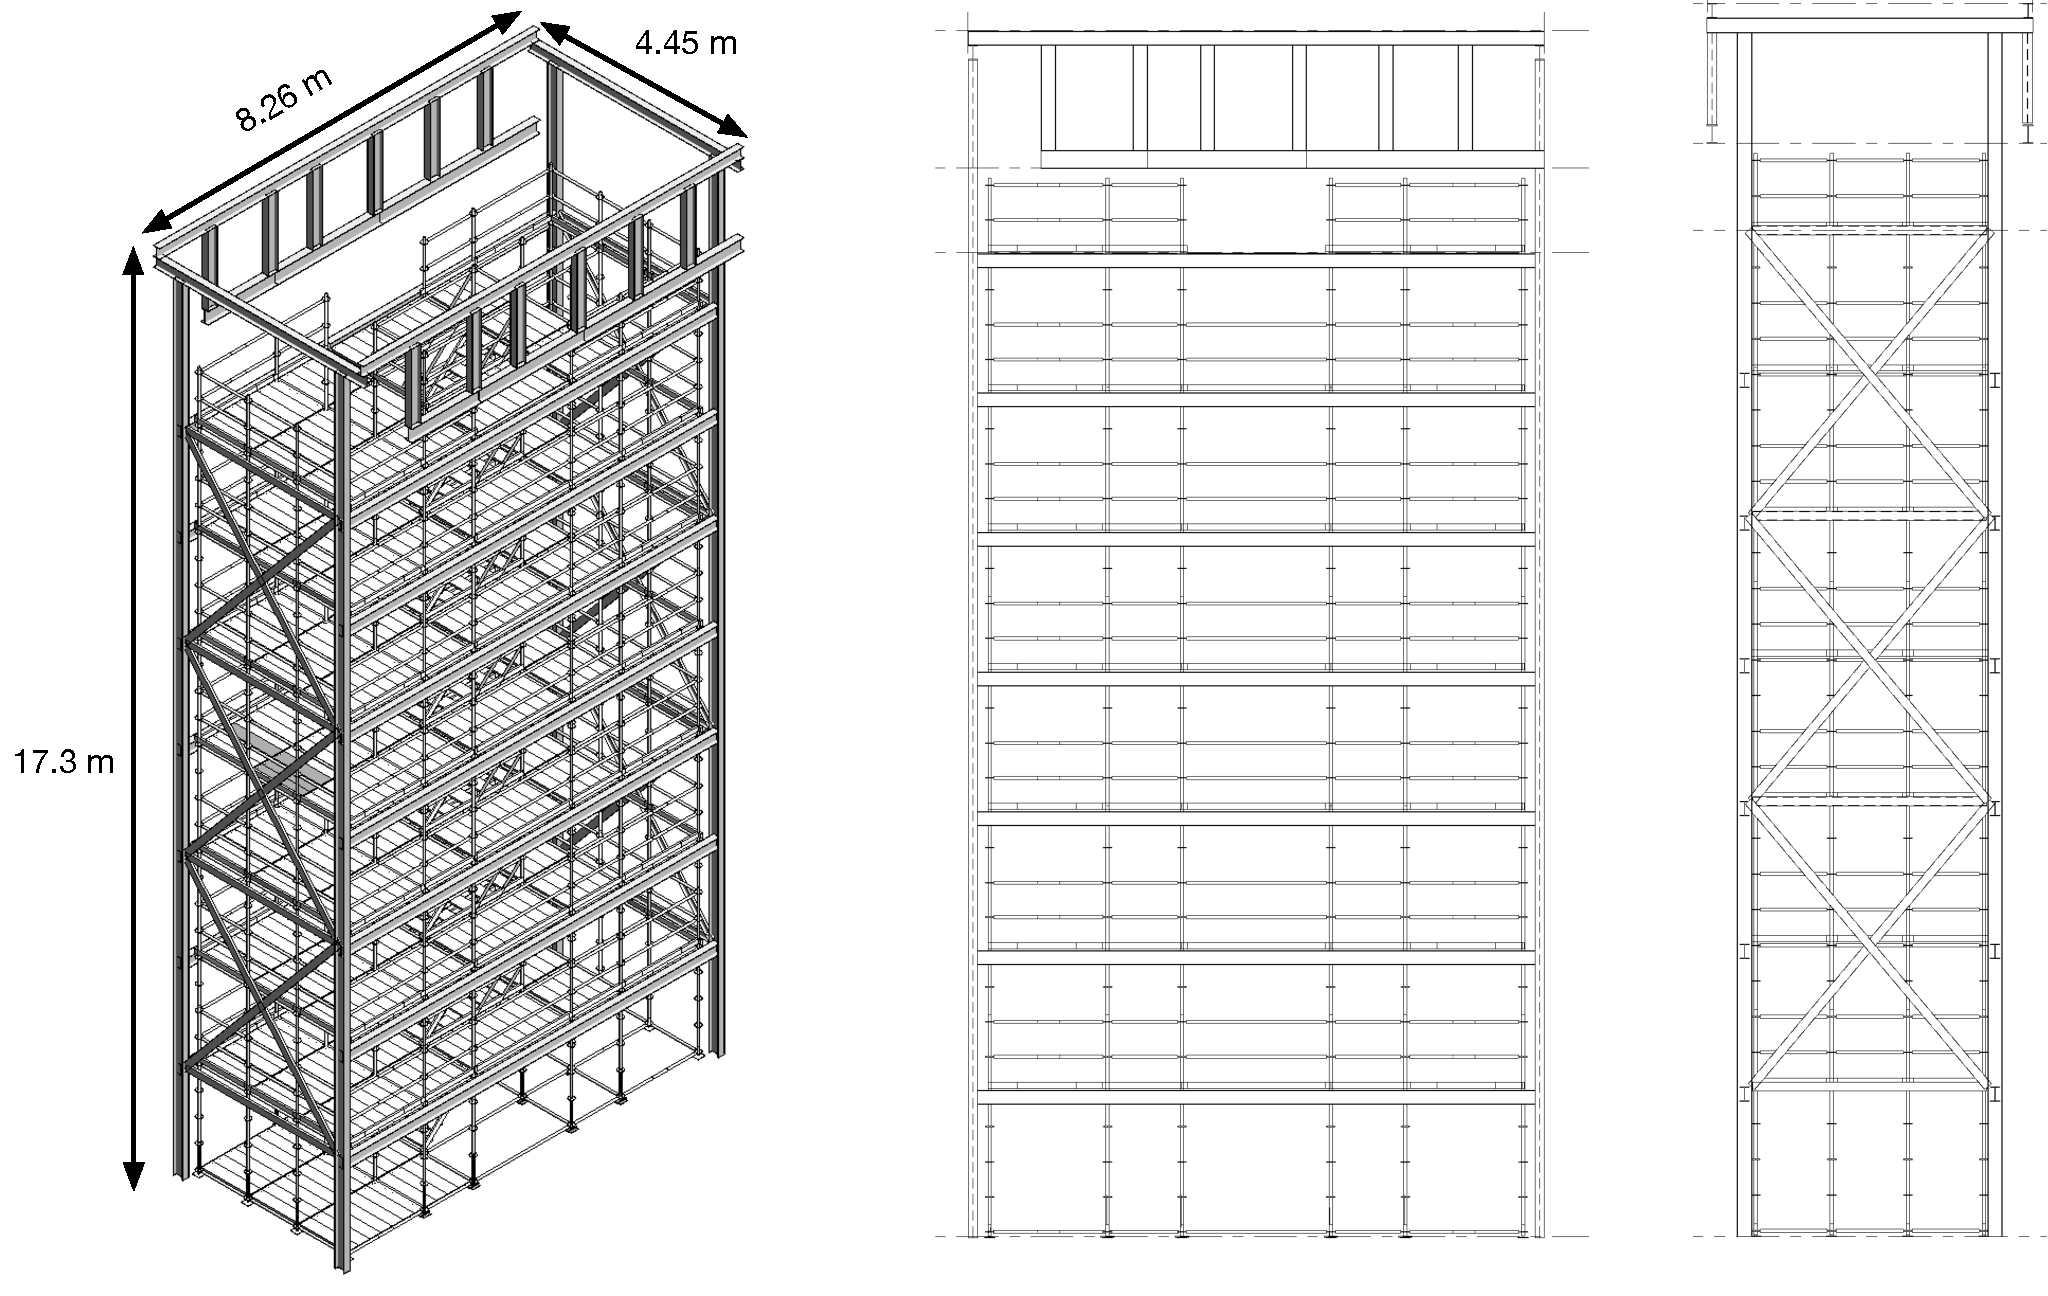
\includegraphics[width=.5\textwidth]{graphics/install-assembly-tower.pdf}
\end{dunefigure}


In the \SI{17}{m} tall  \dword{apa} assembly and cabling area of the cleanroom two large work towers (shown in Figure \ref{fig:install-assembly-tower}) support the four assembly lines. 
These \dword{apa} assembly and cabling towers are where the upper and lower \dword{apa} are assembled together, the \dword{ce} cable is inserted through the \dword{apa} doublet, the cables are connected and arranged for transport, and the electronics are warm tests. 
These towers are designed to be wide enough to hold two \dword{apa} side by side with enough space between to walk through or work. 
The tower is seven stories tall with work areas at each landing.
Rails at mid-height and at the top of the towers are used to move the \dword{apa} to the different locations along the tower. 
The \dword{apa} assembly cabling tower also provides support for the the \dword{apa} assembly fixture provided by the \dword{apa} consortia. 
The \dword{apa} assembly fixture is the tooling needed to hold the upper and lower \dword{apa} during assembly and to bring the two modules together so they can be connected. 
The  tower is conceived as a steel outer frame that supports the \dword{apa}s and the rails. Inside the steel frame is a standard scaffolding for people to use as a work platform. 
The scaffolding allows workers to assess the \dword{apa} at different heights. 
The scaffolding is wide enough for people to be working on both sides simultaneously and for a stairway in the middle that meets OSHA standards. 
North-south beams will be places on top of the tower to support the cleanroom roof and the work platforms shown in Figure \ref{fig:install-workdeck}.
The image shown in Figure \ref{fig:install-assembly-tower} is a modified model based on a single wide \dword{apa} tower which has passed all safety reviews and has already been constructed. 
This double-wide tower will need to be re-engineered to insure that all the beam dimensions and bracing are appropriate for the larger spans and loads. 
It will then go back through the full safety review and the initial prototype of the tower wil be fabricated for use at Ash River. 
The size and the layout of the top level of the tower will be optimized based on input from the Ash River tests. 


\begin{dunefigure}[Cleanroom platforms and material transport system]{fig:install-workdeck}
  {Work platforms, transport rails and switchyard in the installation cleanroom. }
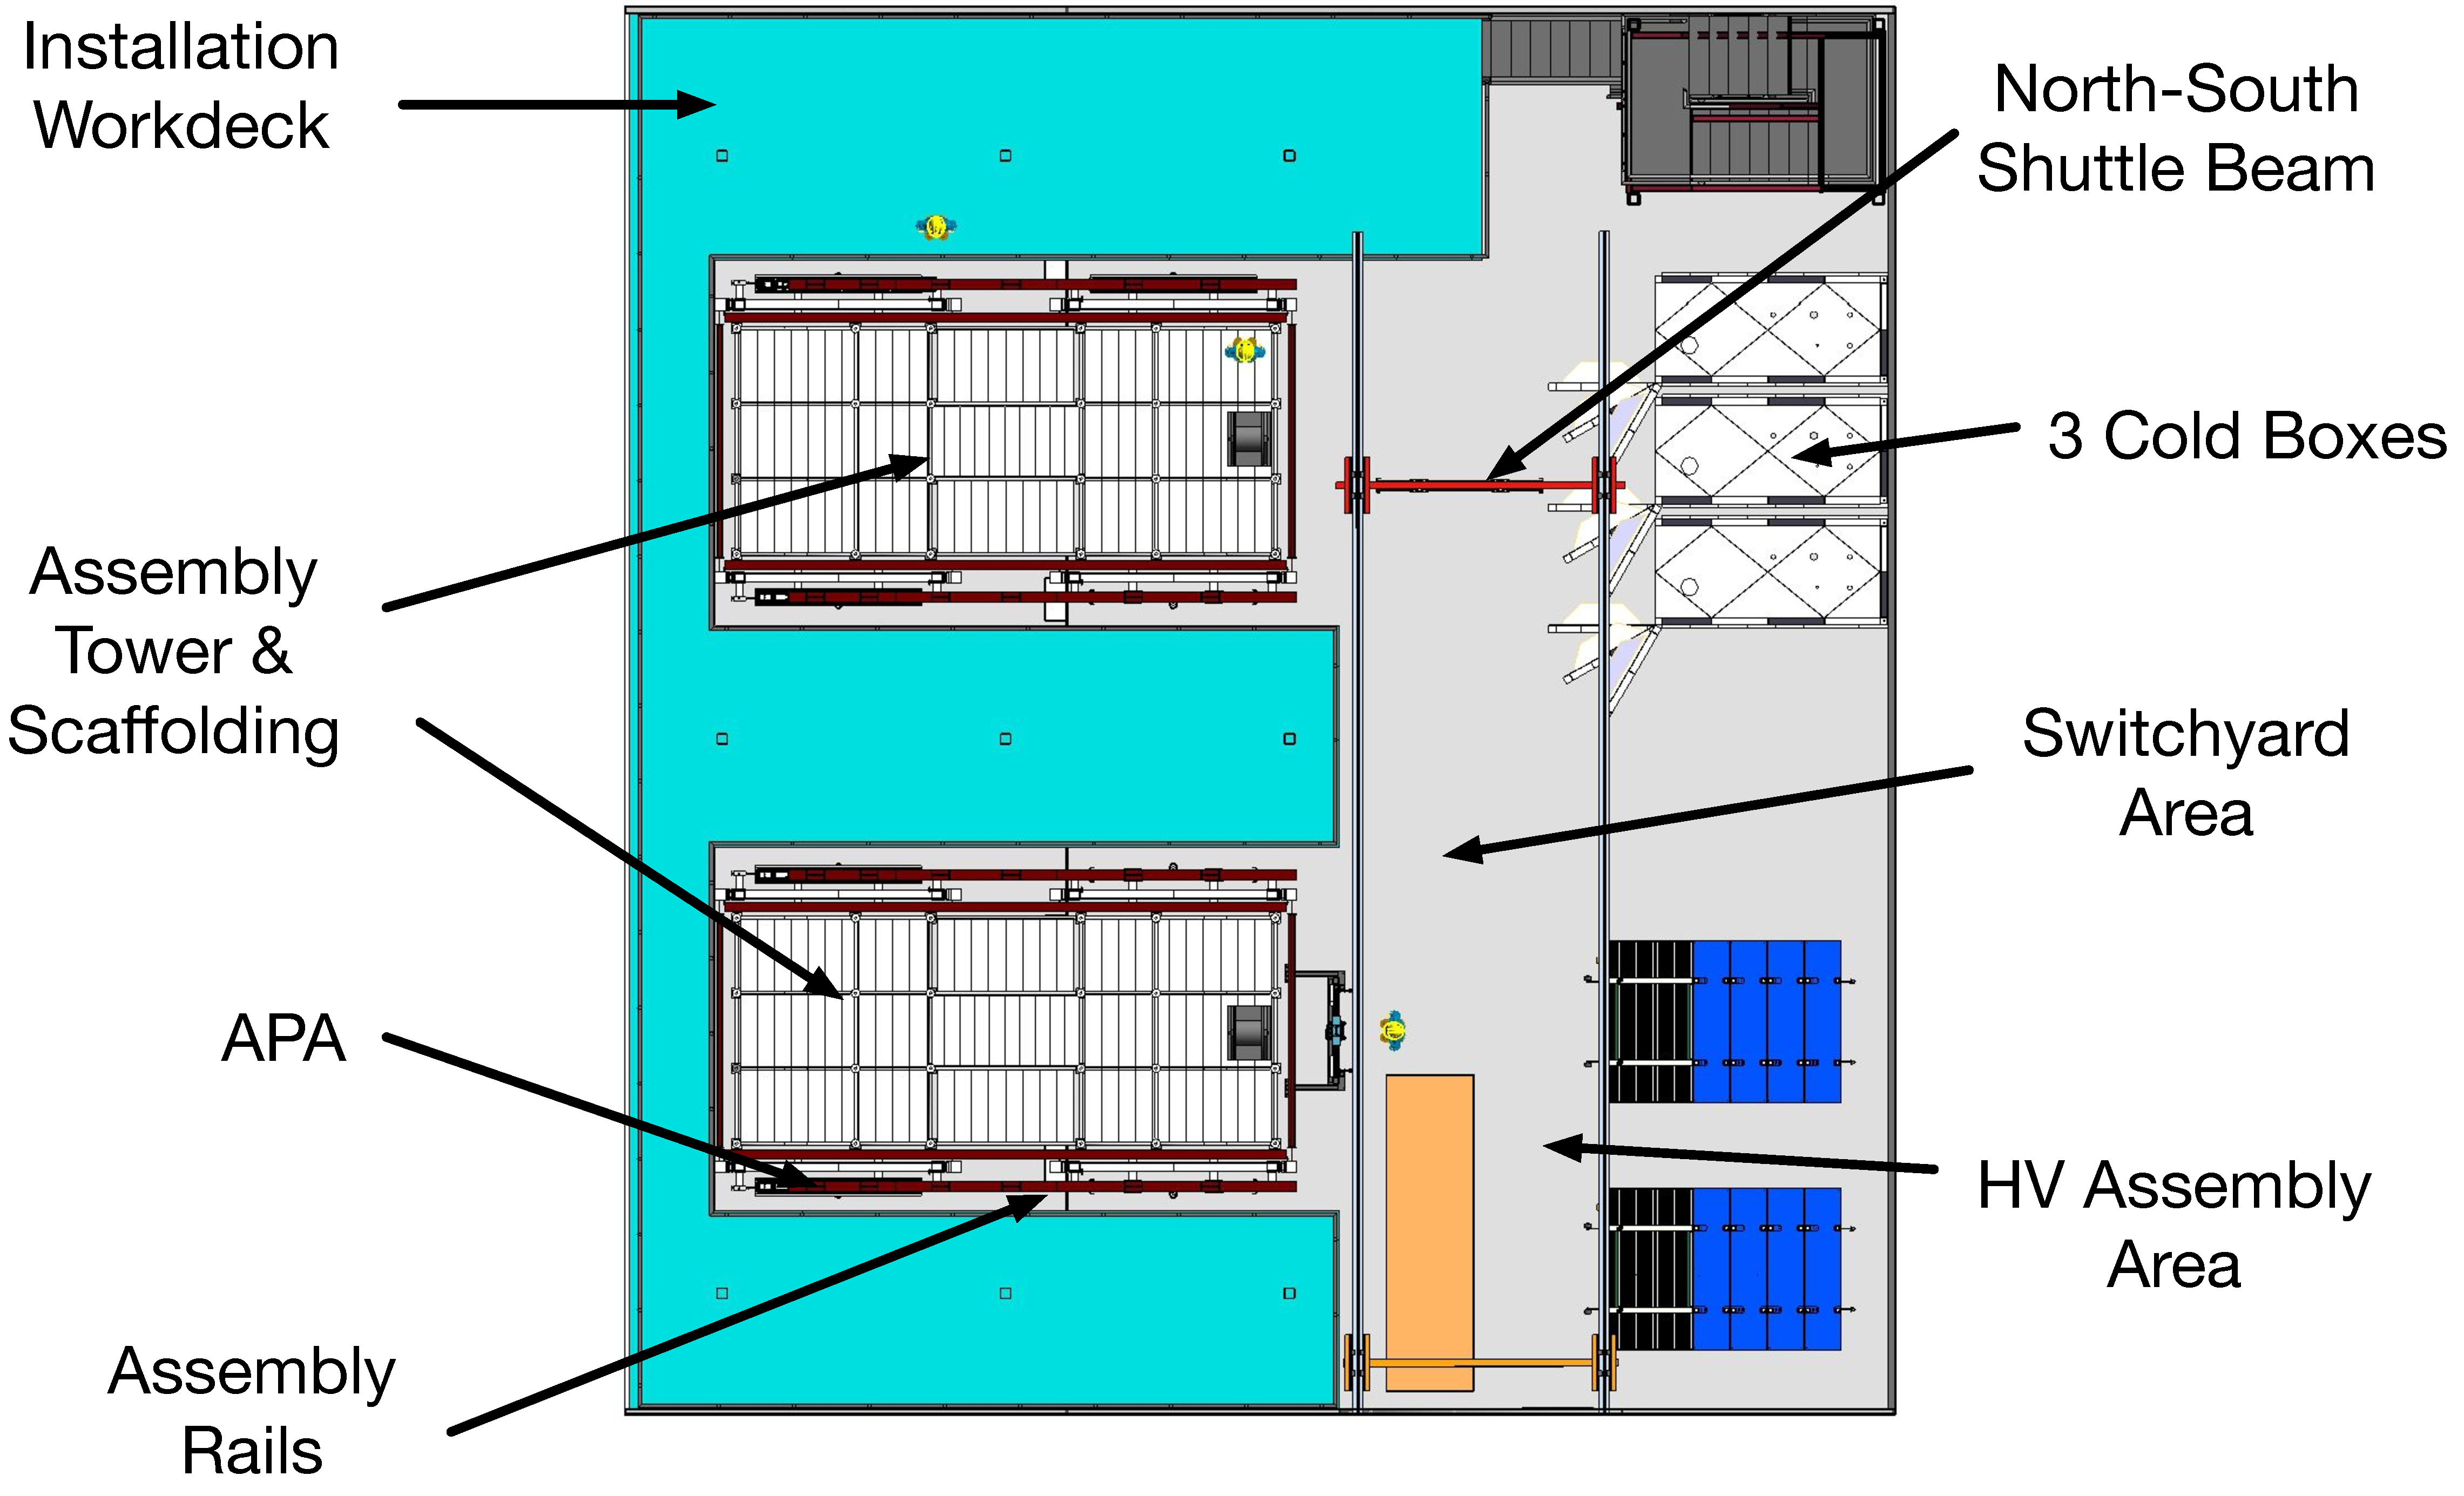
\includegraphics[width=.5\textwidth]{install-workdeck}
\end{dunefigure}

Because the cables can only be inserted through the \dword{apa} frames after the \dword{apa} doublet has been assembled a large amount of work must be performed at the \SI{15}{m} height of the TCO beam. 
\fixme{need to get the height of the TCO beam from the cavern floor.}
The \dword{apa} assembly and testing towers described above provide a solid safe work platform for one side of the \dword{apa}s.
However access to both sides is required to connect the cables to the \dword{femb} and to properly bundle the cable into the cable trays in a way that allows the cables to easily be installed in the cryostat. 
Given the large number of person-hours needed for work at height all measures should be take to ensure that this work is as safe as possible. For this reason a series of stable fixed work platforms will be constructed as shown in Figure \ref{fig:install-workdeck}.
By running north-south beams from the cavern walls across the assembly towers strong rigid support points are provided. 
Vertical posts down from these beams can then support fixed work platforms as needed. Access to the work platforms is provided by a walkway along the west end of the platform which connects to both the assembly towers. A second means of egress is also provided by a connection to the permanent stairs. 




Once the \dword{apa} doublet is assembled it can be moved onto the switchyard under the bridge. 
This switchyard is illustrated schematically in Figure \ref{fig:install-workdeck} is essentially a bridge crane running under the cavern north-south bridge. 
Several bridge beams driven by electric trolleys  move on the runway beams of the crane.  
A rail at the bottom of the crane mates up to the fixed beams  from the assembly lines, the cold boxes, the TCO beams and the HV assembly area.
By aligning the bridge beams with a set of fixed beams supported from the cleanroom roof, the \dword{apa} and \dword{cpa} can be transferred from the fixed beams to the bridge crane and moved to different locations in the cleanroom. 
The \SI{12}{m} tall \dword{cpa} panels will be assembled directly under the bridge crane and transferred directly form the assembly fixture to the switchyard crane.

%%%%%%%%%%%%%%%%%%%%%%%%%%%%
\subsection{Cryogenics and \coldbox{}es}
\label{sec:fdsp-tc-infr-cryo}



After an \dword{apa} pair is fully assembled and cabled but before installation in the detector cryostat, it is thermally cycled in a tall narrow test cryostat, called a \coldbox{}, shown in Figure~\ref{fig:install-coldbox}). 
To test \dword{apa}s at a rate necessary to keep up with the installation plan, we will use three identical \coldbox{}es in the cleanroom. 
The \coldbox{}es require a dedicated cryogenics system that cools them  close to \dword{lar} temperature. 


A \coldbox has external dimensions of 14.0 \si{m} by 3.2 \si{m} by 1.3 \si{m} (H $\times$ L $\times$ W). With three layers of 100 \si{mm} thick foam insulation,  
the internal dimensions are 13.4 \si{m} by 2.6 \si{m} by 0.7 \si{m}. A rail section similar to those used elsewhere in the cleanroom will be mounted inside each \coldbox to allow the cleanroom switchyard and trolleys to push an  \dword{apa}  into a \coldbox. The \coldbox{}es will be light tight when closed to support \dword{pd} testing. A support base under the \coldbox{}es will adjust the height to mate with the cleanroom switchyard.

 
The \coldbox electronics \fdth{}s  will be  similar to what is used on the top of the \dword{dune} cryostat, except that short cables will be run from the \dword{wec}  to a patch panel inside the \coldbox. This will allow the cable on the \dword{apa} to connect directly to the test readout without having to remove any cabling. The \coldbox  design is nearly the same as the successful \dword{pdsp} \coldbox. The outer shell is similarly constructed of a stainless steel plate with reinforcing ribs welded on. The height is of course doubled, and a hinged door is planned. Unbolting the door and lifting it off the \dword{pdsp} \coldbox required significant effort, and lacking full crane coverage in this case, doors that can be opened and closed using a scissor lift are necessary. The \dword{dune} \coldbox{}es will collectively need about 11 \si{T} of stainless steel, according to initial estimates. The \coldbox{}es may be assembled in place because the finished boxes are too big to fit down the Ross Shaft. As the design continues it will be investigate if the boxes can be assembled in pieces that can be brought underground separately and assembles. The \coldbox base will be on Hilman rollers, so the boxes can be moved under the bridge after detector installation  to allow installation of the cryogenic circulation pumps.




\begin{dunefigure}[Installation \coldbox]{fig:install-coldbox}
  {\coldbox{}es used to thermally cycle the fully assembled APA pairs. }
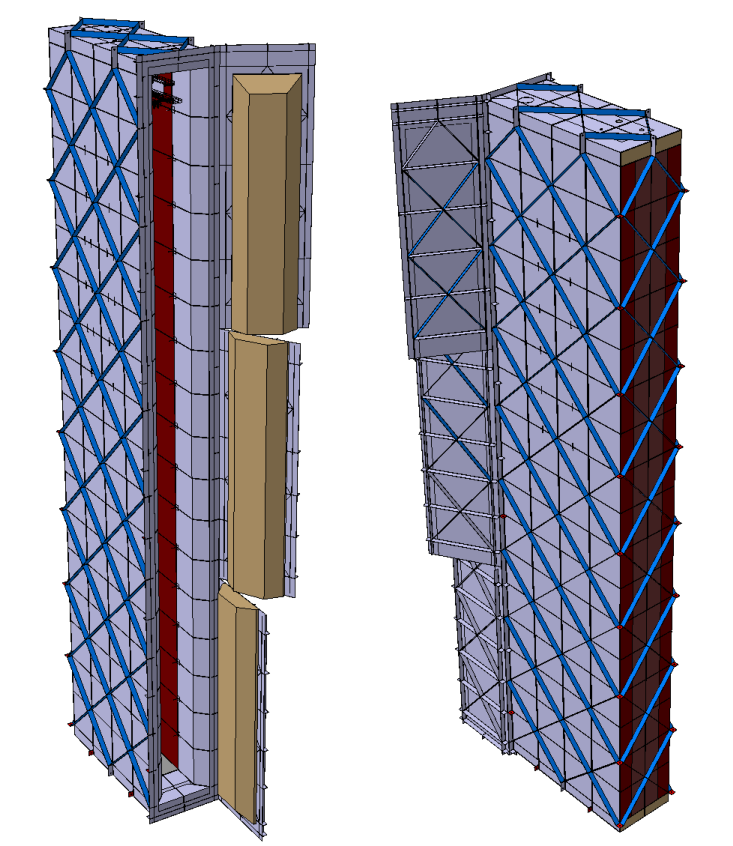
\includegraphics[width=.5\textwidth]{graphics/install-coldbox.pdf}
\end{dunefigure}


%{Cold Boxes Cryogenics}
\label{sec:fdsp-tc-cryocoldbox}

%The cryogenics supporting the \coldbox{}es underground must ensure reliable and safe operation of the system used to test the \dwords{apa} that will be installed inside the cryostats. The main functional requirements of the system are
The  \coldbox{}es will be used to test the \dword{apa}s underground prior to installation. % in the cryostat. 
The cryogenics supporting the \coldbox{}es  must ensure their reliable and safe operation; to that end, it must
\begin{itemize}
\setlength\itemsep{1mm}
\setlength{\parsep}{1mm}
\setlength{\itemsep}{-5mm}
\item support three \coldbox{}es operating in parallel: %for testing dual \dword{apa}s: 
one in \cooldown mode, two either in steady-state or warm-up modes.
\item allow personnel in the cleanroom during all phases of the purge, \cooldown, operation, and warm-up modes. 
\item test the detector modules at near \dword{lar} temperature.
\item operate 24 hours a day, seven days a week for 10 years.
\item allow remote operations.
\item be located in the vicinity of the \dword{tco}. Space is available on top of the cryogenic mezzanine on the roof of the cryostat.
\end{itemize}

It must operate in the following modes: %fulfill the following modes of operations:

\begin{itemize}
\setlength\itemsep{1mm}
\setlength{\parsep}{1mm}
\setlength{\itemsep}{-5mm}
\item \textbf{purge}: During this mode, air is removed from the system (\coldbox and cryogenic system) and replaced with dry nitrogen. The concentration of moisture is monitored, and when it no longer decreases, the \cooldown can commence.
\item \textbf{\cooldown}: Cold nitrogen is introduced into the system to cool the inside of the \coldbox and the \dword{apa} inside it. %it down and to cool down the detector contained inside the coldbox. 
This should take 24 hours, during which time the temperature decreases from room temperature to about \SI{90}{K}. 
\item \textbf{steady-state operations}: After reaching %the nominal temperature of 
approximately \SI{90}{K}, %the value is maintained for 48 hours, during which 
the detector is turned on and fully tested. % at cold. 
This takes about 48 hours.
\item \textbf{warm-up}: After completing the test, the system is %slowly 
warmed up to room temperature over a period of 24 hours. %This should take 24 hours, during which the temperature goes from approximately \SI{90}{K} to room temperature.
\end{itemize}

\begin{dunetable}
[\Coldbox  cryogenics system parameters] %for specifications]
{lc}
{tab:table-cryo-coldboxes}
{Table of parameters for the \coldbox cryogenics system.}
Parameter & Value 
\\ \toprowrule
Dual \dword{apa} thermal mass &  1,600 kg\\ \colhline
Temperature uniformity & $+60$ K / $-0$ K \\ \colhline
Electronics load & 300 W \\ \colhline
\Coldbox insulation thickness &  0.3 m \\ \colhline
Target \cooldown temperature &  \SI{90}{K} \\ \colhline
Target \cooldown duration &  24 hr \\ \colhline
Target steady-state duration &  48 hr \\ \colhline
Target warm-up duration &  24 hr \\ \colhline
Maximum cooling power  &  \SI{13}{kW}  \\ \colhline 
Maximum liquid nitrogen consumption  &  \SI{300}{l/hr}  \\ \colhline 
\end{dunetable}

The evaporation of liquid nitrogen provides the cooling power for the system. Warm nitrogen and a heater provide the heating power. At peak consumption, the expected maximum heat load is \SI{8.5}{kW}. Assuming a 50\% margin on the refrigeration load, the cryogenics system requires \SI{13}{kW} of net cooling power at peak consumption, which equals about \SI{300}{l/hr} of evaporating liquid nitrogen.

Two layouts are currently under consideration: (1) a closed loop with mechanical refrigeration, in which liquid nitrogen is generated {\it in situ}, circulated, and the spent nitrogen recondensed before being put back into the system; and (2) open loop, in which liquid nitrogen is transported underground by means of portable dewars, circulated, and the spent nitrogen vented away. For the closed loop, we would need a mechanical refrigeration capable of supplying \SI{13}{kW} of cooling. For the open loop, it is possible to use a \SI{2000}{l} dewar, which is commercially available and transportable up and down the Ross Shaft inside the cage. To supply the required amount of nitrogen, four trips per day are needed.

The current versions of the closed loop and open loop systems are presented in Figures~\ref{fig:mechanical-refrigeration} and~\ref{fig:LN2}, respectively. % . The current version of the open loop system is presented in Figure~\ref{fig:LN2}.

\begin{dunefigure}[\Coldbox cryogenics support system based on mechanical refrigeration ]{fig:mechanical-refrigeration}
  {Layout of the cryogenics supporting the \dword{apa} test facility with mechanical refrigeration (closed loop).}
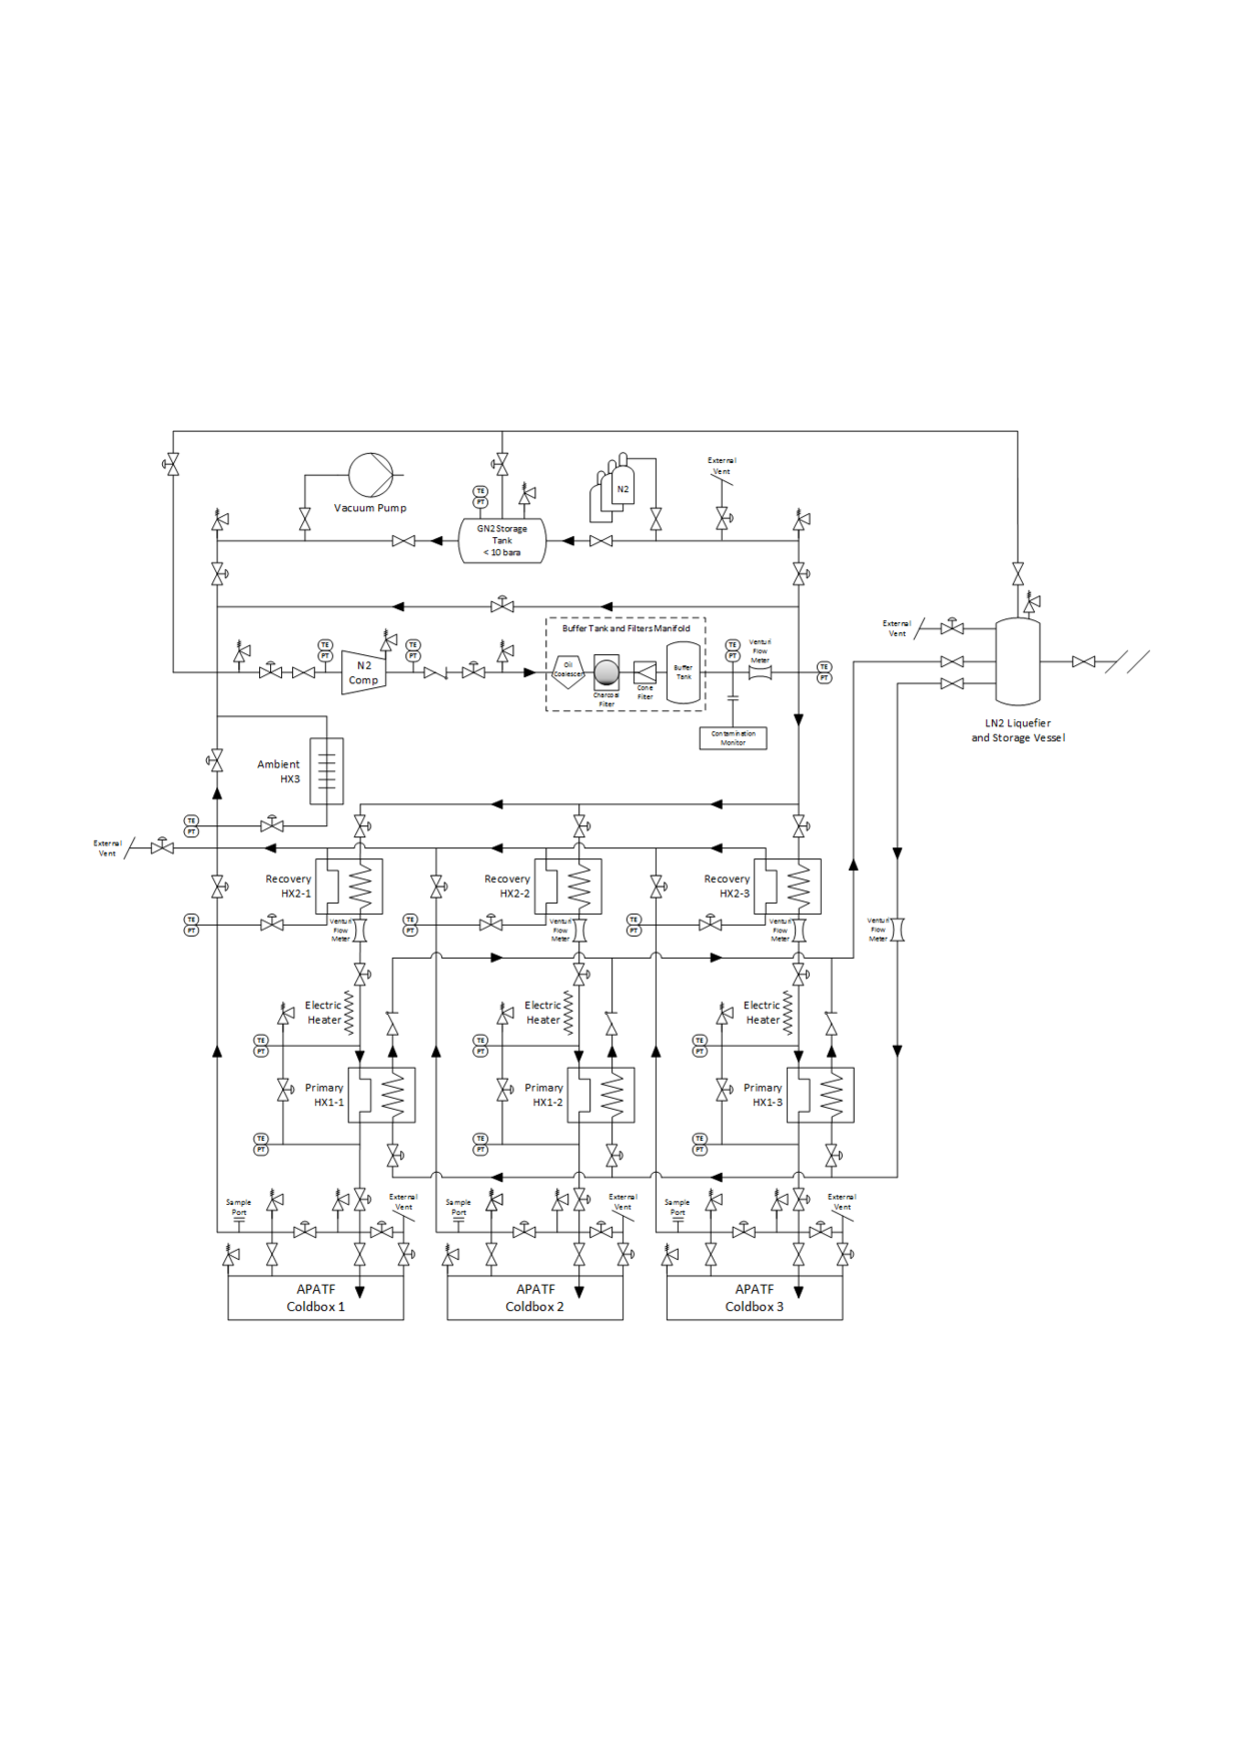
\includegraphics[width=.98\textwidth]{graphics/Cryo-cold-box-mechanical.pdf}
\end{dunefigure}

\begin{dunefigure}[\Coldbox cryogenics support system based on LN2 ]{fig:LN2}
  {Layout of the cryogenics supporting the \dword{apa} test facility with open loop refrigeration (open loop).}
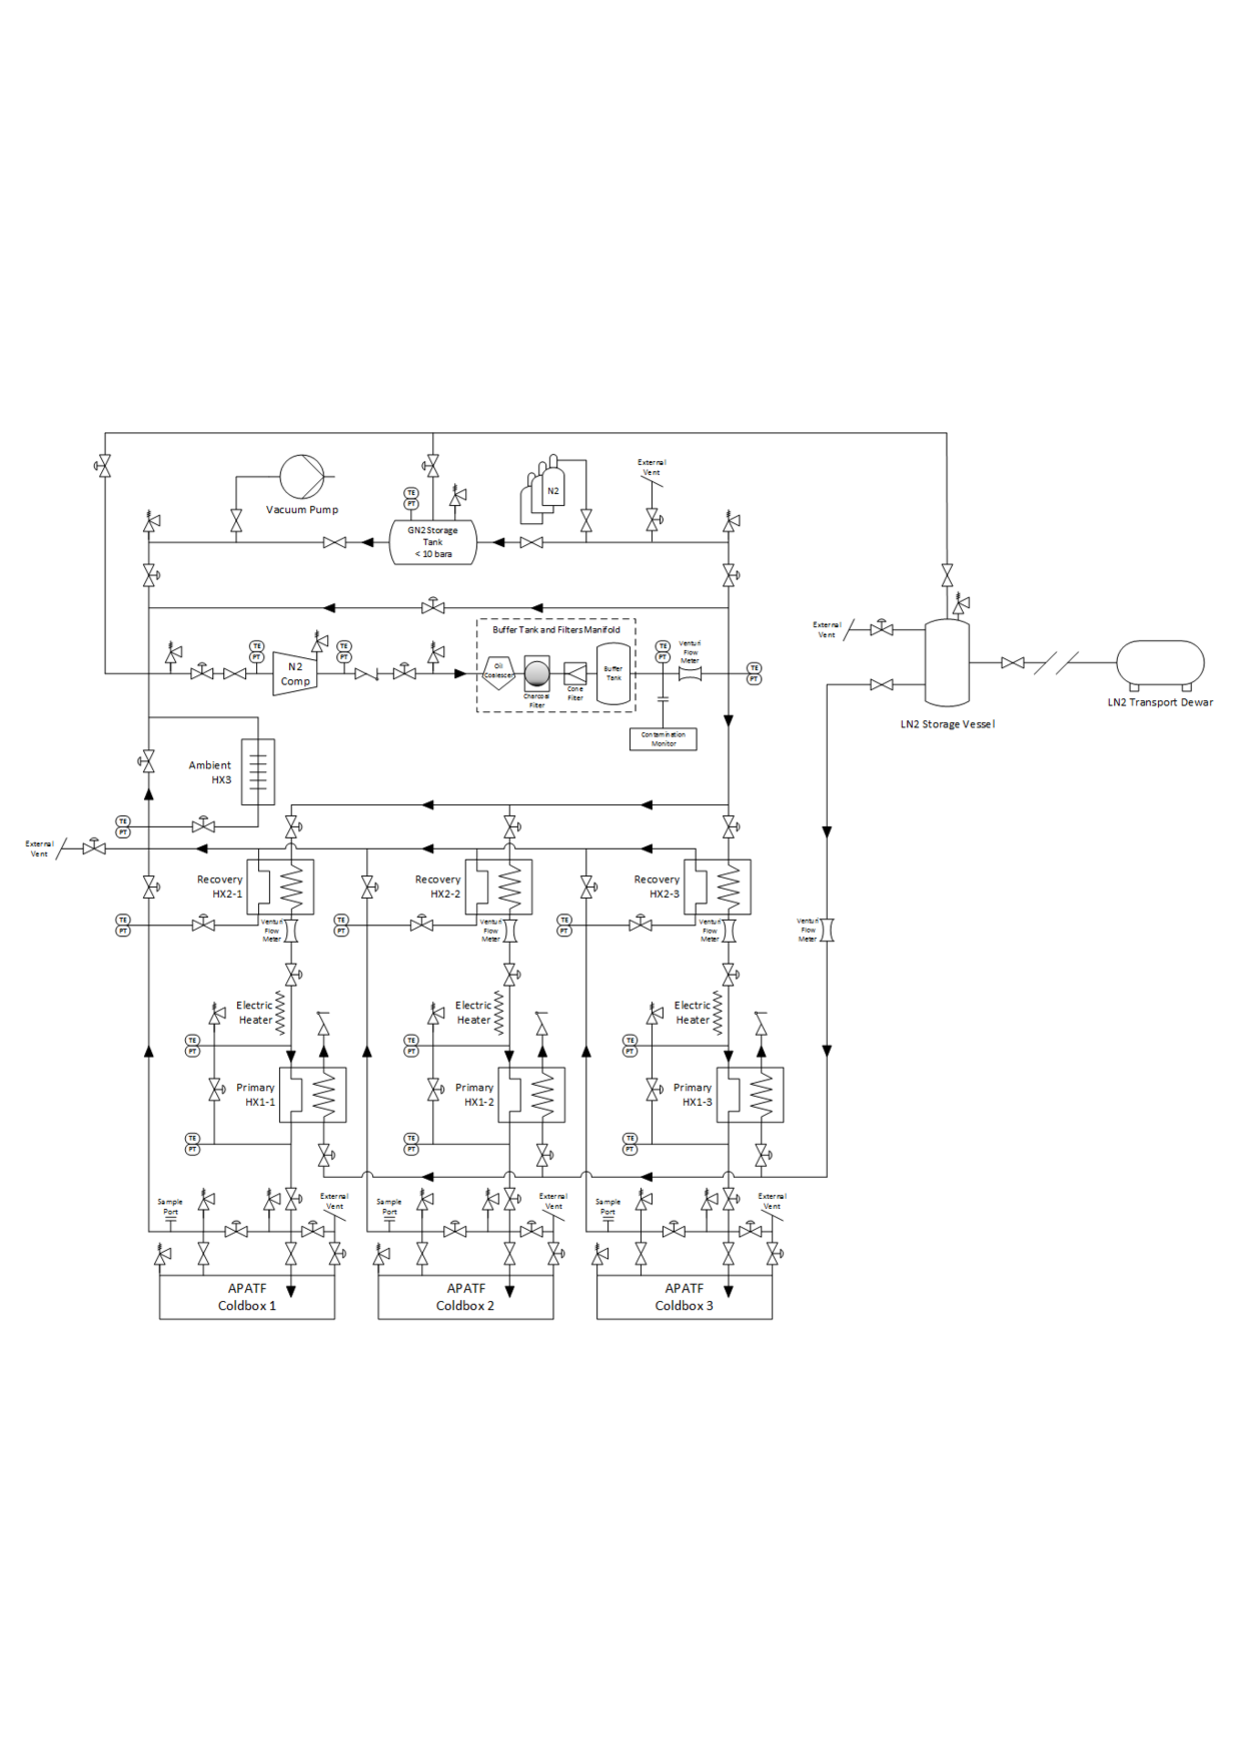
\includegraphics[width=.98\textwidth]{graphics/Cryo-cold-box-LN2.pdf}
\end{dunefigure}



%%%%%%%%%



%%%%%%%%%%%%%%%%%%%%%%%%%%%%
\subsection{Prototyping and Testing (QA/QC)}
\label{sec:fdsp-tc-infr-qaqc}


Installing all this new equipment underground during the installation setup phase involves a lot of new techniques  and unique work. While most of the procedures will have been tested during the trial assembly at Ash River, everything must be properly approved. The main \dword{apa} and \dword{cpa} towers will already be structurally approved, but all lifting fixtures, shuttle beams, crane tower connections, and \coldbox connections must undergo load tests. 

The load test program for the lifting fixtures, shuttle beams, crane tower connections, and cold box connections will be documented in test procedures in accordance with the LBNF DUNE QA Program.  
These test procedures will include pre-requisites prior to testing, identify fixtures and test equipment, step by step instructions, acceptance criteria and documentation requirements. 
This process will be in place prior to the start of testing. 
The test results will be documented and approved by the Systems Engineering prior to use of the lifting fixtures, shuttle beams, crane tower connections, and cold box connections must undergo load tests.

The \coldbox{}es and cryogenic system will also be tested, so access to the cleanroom  may be restricted for several days for system checks. 
The cold boxes and the associated cryogenic system test program will be similar to the test program that was instituted for \dword{protodune}. 
The test program will be documented in procedures in accordance with the LBNF DUNE QA Program. The test procedures will include pre-requisites prior to testing, identify test equipment, step by step instructions, acceptance criteria and documentation requirements. The test results will be documented and approved by the Systems Engineering prior to use of the cold box and cryogenic system.


% clear the figure buffer before starting the next section
\clearpage

% Note: infrastructure.tex inputs dss.tex

%%%%%%%%%%%%%%%%%%%%%%%%%%%%%%%%%%%%%%%%%%%%%%%%%%%%%%%%%%%%%%%%%%%%
%\section{Detector Installation}
%\label{sec:fdsp-tc-inst}

\section{Detector Installation}
\label{sec:fdsp-tc-inst}

\subsection{Introduction}
\label{sec:fdsp-tc-inst-intro}

The DUNE detector installation will proceed in three phases the CUC setup phase, the installation setup phase, and the detector installation phase. The CUC setup phase is the first step in the installation process. The start of the CUC setup phase begins when the underground area for the North Cavern and Central Cavern become available to LBNF and DUNE. At this time the cryostat construction can begin in The North Cavern and equipment installation can begin in the Central Cavern or the Central Utility Cavern (CUC). The main equipment from DUNE which is installed in this phase is the equipment in the DUNE dataroom. The detector installation setup phase begins during the cryostat membrane installation period. In this phase the equipment needed to perform the detector installation will be erected in North Cavern. This includes the installation of the bridge across the cavern, the installation cleanroom, lifting equipment and work platforms, the cold boxes and cryogenic system for testing APA, and the DSS with related switchyard. In the third phase of the installation the detector itself will be installed. The work in each phase will be described the following sections.

\begin{dunefigure}[Layout of the underground area]{fig:cavern-layout}
  {Top view of the layout at the 4850 level at SURF. Shown are the 3 large excavations and the location of detectors in excavation \#1 and \#3. Excavation \#2 is the CUC which houses the DUNE dataroom and the underground utilities.}
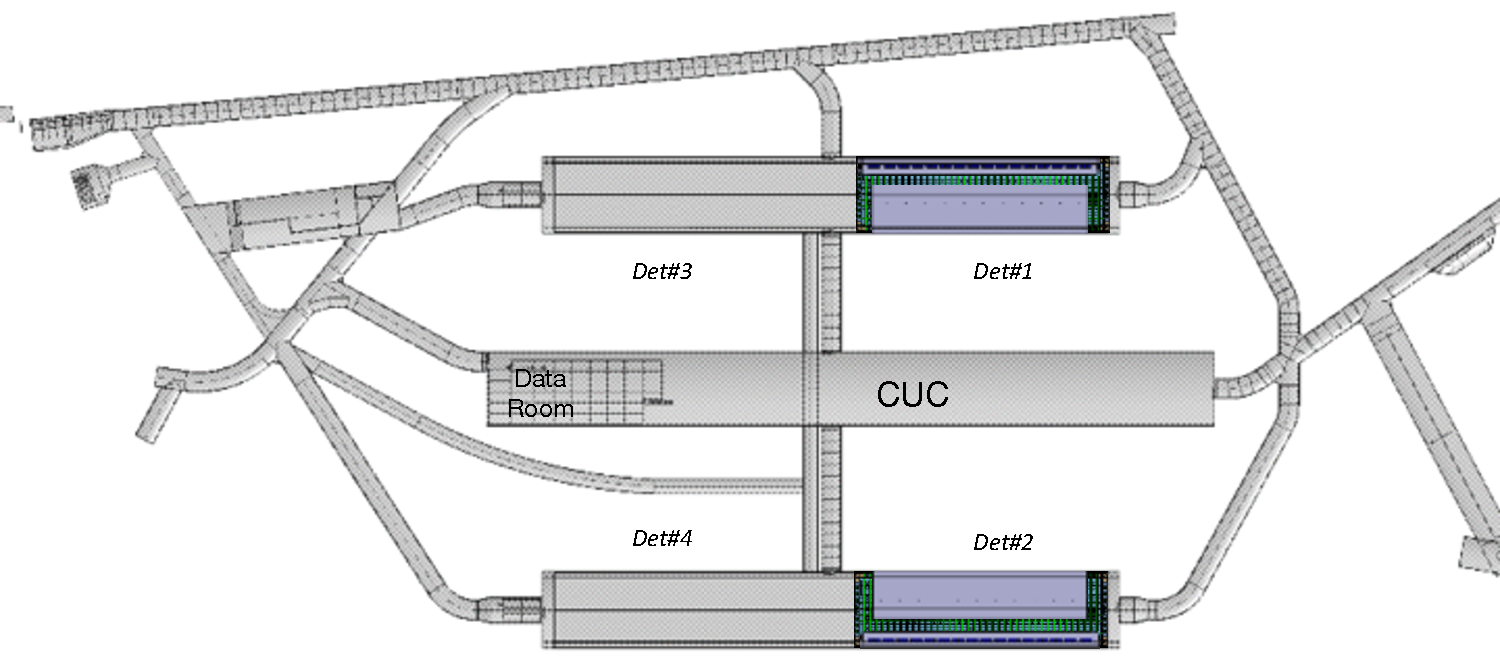
\includegraphics[width=.9\textwidth]{cavern-layout}
\end{dunefigure}

\fixme{insert very simple schedule}

%%%%%%%%%%%%%%%%%%%%%%%%%%%%
\subsection{Installation Process Description}
\label{sec:fdsp-tc-inst-proc}

\subsubsection{CUC Installation Phase}

\begin{dunefigure}[Layout of the DUNE dataroom and experimental workarea in CUC]{fig:install-cuc}
  {TOP: The overall layout of the DUNE spaces in the CUC is shown. The inner room is the DUNE dataroom which houses the underground computing and the outer area referred to as the experimental workarea is a general purpose workarea. Bottom: The first row of racks in the data room is shown. The first two racks are the  CF interface racks. The image was taken from the ARUP design drawing U1-FD-T-701}
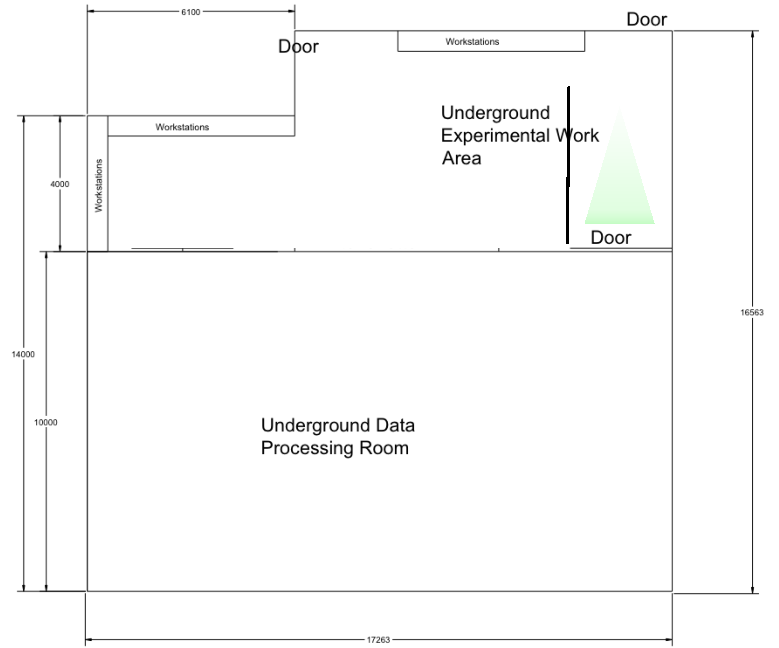
\includegraphics[width=.7\textwidth]{cuc-layout}
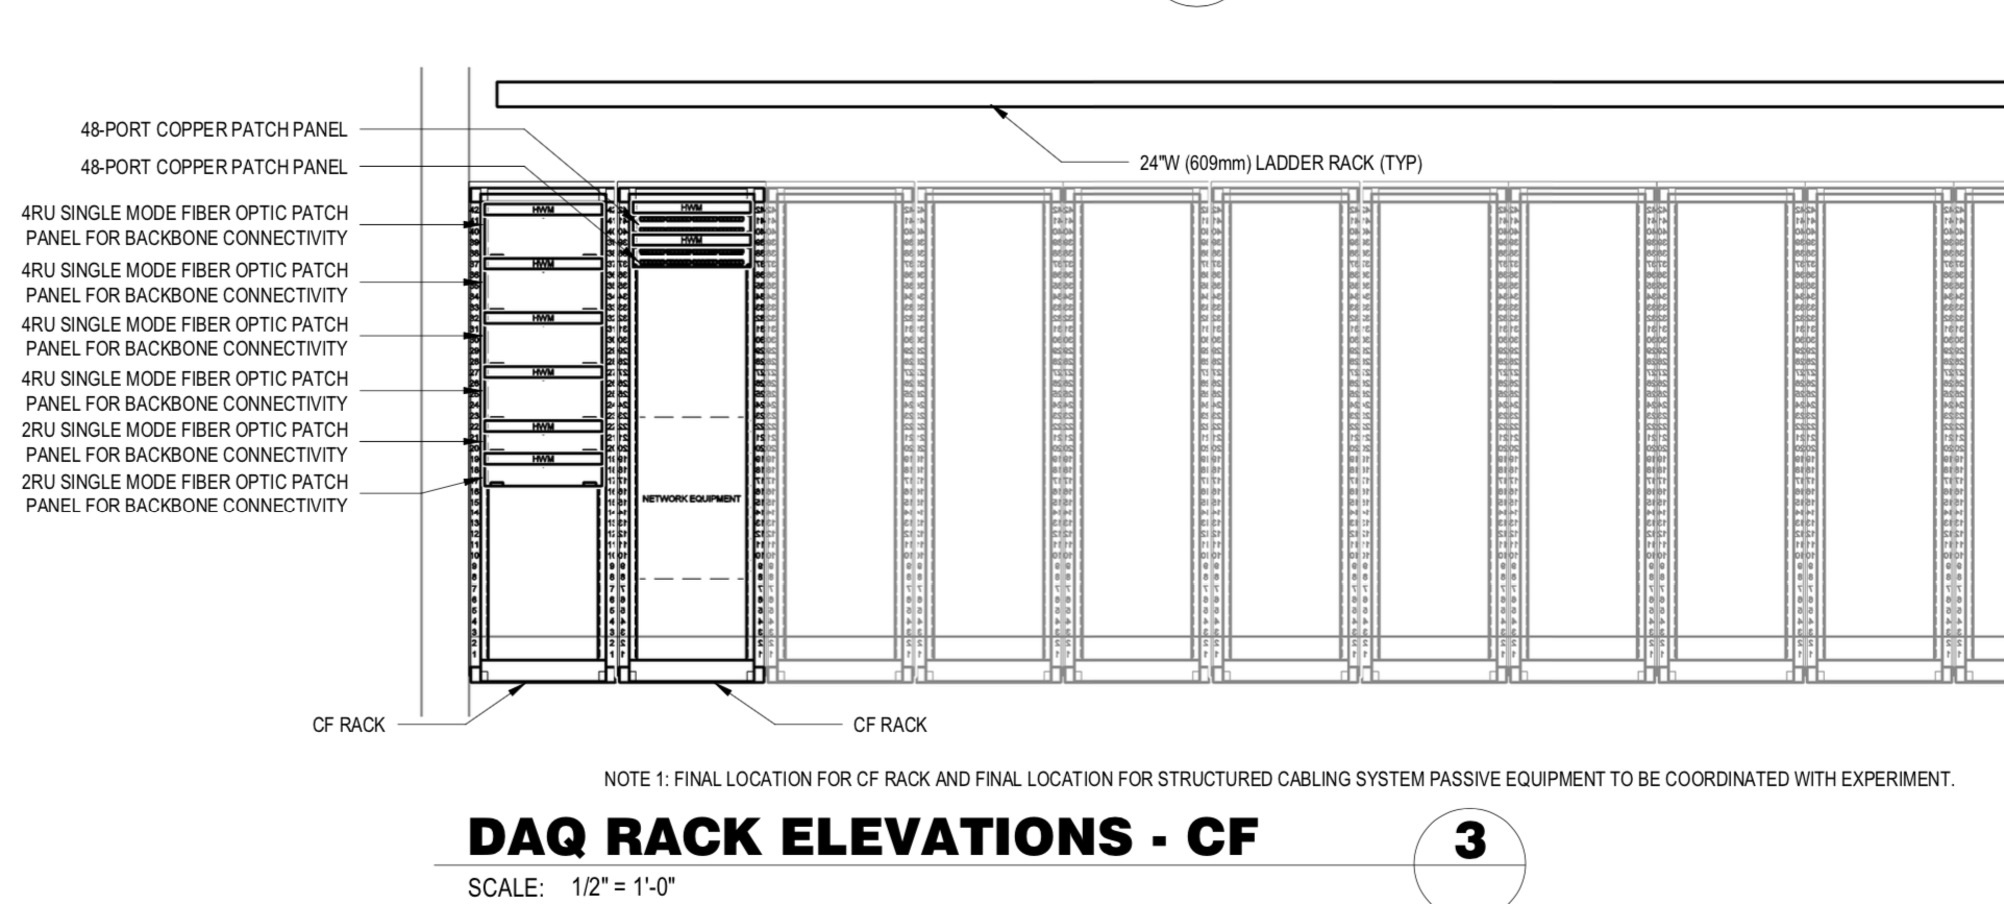
\includegraphics[width=.9\textwidth]{cuc-cf-racks}
\fixme{need to use a figure from the 90\% submittal}
\end{dunefigure}


The first stage of the CF work ends when the outfitting of 
the North and Central caverns is complete. At this time the CUC is ready for DUNE outfitting and the cryostat installation can start for detector 1. During this period DUNE will not have assess to the detector excavations as the heavy steel work for the cryostat will be ongoing. The only work planned for DUNE in this period is the outfitting of the data room and work area room in the CUC shown in Figure \ref{fig:install-cuc}. CF will provide the empty room with an 18 in false floor, a 500KVA power disconnect, and connections for chilled water sufficient to cool the racks. The dataroom like the adjacent CF electronics room will be outfitted with a dry fire extinguishing system. 

The water cooled racks, cable trays, power distribution, and water distribution are the responsibility of DUNE and will be installed once the space becomes available. The installation of the racks needs to be coordinated with CF as the first two racks are for CF usage and need to be in place before the underground phase one work is complete. Some small overlap will be needed between CF and DUNE at this time.

At the same time the eight DAQ racks which receive the data from the underground area and then transmit the data to FNAL will also be installed. With this infrastructure in place the DAQ group can begin constructing and testing the final DUNE DAQ.  

The underground experimental work area is a general purpose area that will need to serve many purposes during the DUNE installation. Initially the area will be outfitted with office equipment for the installation team, workstations for DAQ, and a basic conference area for meetings.  The room is 4-6.4 \si{m} deep and 20 \si{m} long so it can serve several functions.

During this early installation stage the machine shop and DUNE storage area will also be setup in the detector excavation area.

\subsubsection{Installation Setup Phase}

Once the steel structure of the cryostat is complete the remaining work will be focused inside the cryostat. 
There will still be a lot of activity outside the cryostat as the 4,000 crates of foam and other materials are transported inside but the outer structure will be in position so some DUNE work can start. 
The first piece of equipment to installed will be the bridge between the North and South drifts. 
This will allow the cryogenics equipment to travel from the North drift to the CUC and will provide part of the structure for the cleanroom. 
Construction of the cleanroom frame and related hoisting equipment can then begin. 
The largest most complex equipment that must be constructed in this phase are the cold boxes and related cryogenics system. 
Due to the size of the cold boxes these must be constructed in place. 
The layout of the installation region outside the cryostat is shown in Figure \ref{fig:install-ug-layout}. 
This figure shows a cut below the bridge so the majority of the installation equipment can be seen. 
The three 15 \si{m}tall cold boxes are seen in blue next to the yellow access stairway. 

The hoisting equipment and the rail system needed to move the detector components in the installation area interfaces with the bridge, cryostat and possibly the cleanroom mechanical structure. 
Installing this early will make transporting equipment around the area outside the cryostat significantly simpler. 
\fixme{Do we want a figure of just the rails and switchyard?} 
The assembly towers for the APA assembly, APA cabling, and CPA assembly can be installed when it is most convent for the cryostat installation crew. 
Just prior to the start of detector installation the cleanroom walls will be installed, the area will be cleaned and added filters will be installed to convert the area to an ISO-8 cleanroom.

During this phase of the cryostat installation the majority of the cryostat work will be inside an at the 4910 level. 
This will allow significant work to be performed on the cryostat roof for the cryogenic system installation and the detector installation setup. 
The cryostat crossing tubes will be installed on the roof 
\fixme{figure of the cryostat crossing tube with the mechanical connection to the I-beams and the inteface to the membrane.} . 
These assemblies are welded to the 1 \si{cm} thick steel cryostat roof and are then additionally cross braces to the large I-Beams. 
The thick walled tubes which penetrate through the foam insulation are in place at this time. 
Once the crossing tubes are in place the large tees for the cold electronics can be installed. 
The next step in the installation requires the internal roof of the cryostat to be complete. 
At this time the DSS support feedthrus can be installed and possible the DSS beams can be lifted into positions. 
The details of how to coordinate this work will be iterated with the cryostat manufacturers as the design work is completed. 
At this time the cold electronics mechanical feedthrus can be installed. 
Once work on the feedthru are complete then the mezzanines for the cryogenic system and the detector electronics racks can be installed.
Finally the cable trays,  piping, lighting, and cryostat roof flooring are installed. 
At this time the cryostat roof is ready for the start of the DAQ installation in the detector area.

The last steps in the installation setup phase is the installation of the cryostat internal piping, cleaning the cryostat, installing the false floor, and filtered lighting to protect the photon detectors. 
\fixme{ Insert the figure of the piping inside the cryostat. }



\subsubsection{Detector Installation Phase}

\begin{dunefigure}[Top view of the installation region inside the cleanroom ]{fig:install-cleanroom-layout}
  {Top view of the cleanroom used for installation. In this view cleanroom roof and bridge are not shown. The equipment used for the installation is shown along with the material airlock layout and the location of the changing room. The cryostat is to the right of the figure and the I-Beams passing through the TCO opening are shown.}
 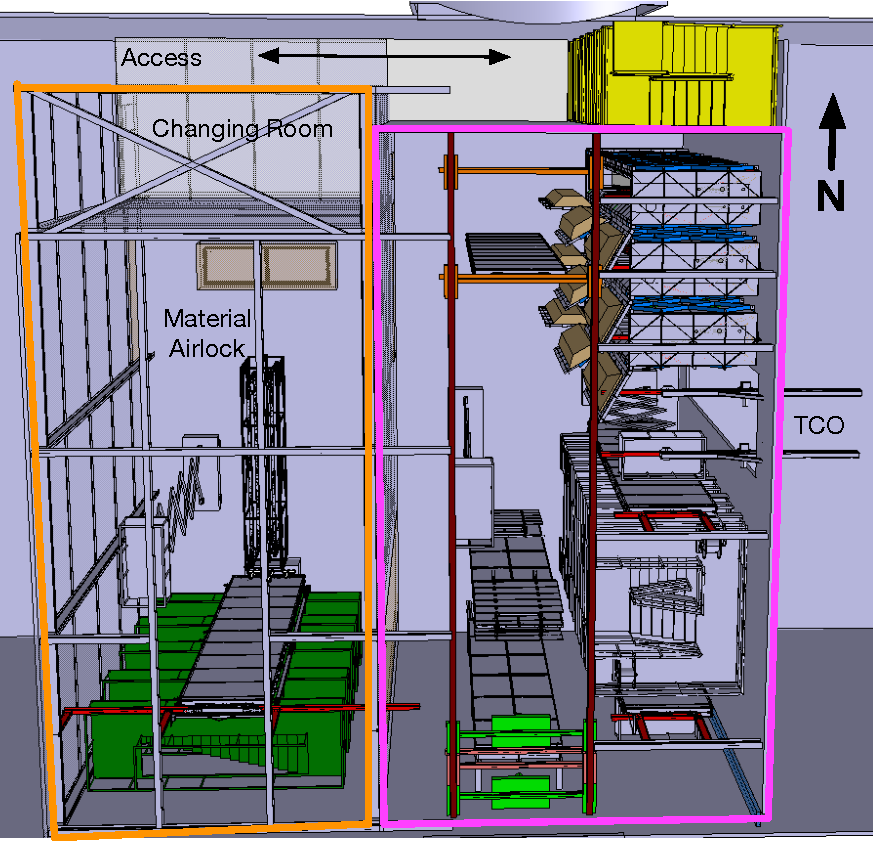
\includegraphics[width=\textwidth]{install-cleanroom-layout}
\end{dunefigure}

At the start of the detector installation phase the work on the cleanroom is complete, the DSS is installed in the cryostat including the switchyard near the TCO. 
The light in the cryostat and cleanroom will be filtered to protect the photon detectors and the air will be filled to reduce the dust collected during installation. 
The cryogenic piping will be in place along with the false floor. 
The false floor both gives a flat work area and protects the 1.2 \si{mm} thick stainless steel cryostat membrane. 

The layout of the cleanroom during the detector installation phase is shown in Figure \ref{fig:install-cleanroom-layout}. This image is a top view of the cleanroom with the roof and bridge removed; the cryostat is on the right and the open cavern on the left. In the North-East corner of the figure the access stairway is shown in yellow. This stairways is outside the cleanroom and allows people to access the 4910 level from the North drift or from the cryostat roof. An access corridor along the north wall connects the stairway to the rest of the cavern. The changing room and airlock are found on the West of the figure and are outlined in orange. The changing room is located in the the North-West corner and provided access to both the cleanroom and the airlock. South of the changing room is the material airlock. This rather large area is where the APA modules are connected together to form the 12 \si{m} tall units. The assembly station is shown in green along the south wall of the airlock. This area is also where all the materials are brought from the dirty outside cavern and are cleaned or the outer packaging removed. Roll-up doors along the West wall allow material from the outer cavern to be brought into the airlock. A section of the roof can be removed to allow the cavern bridge crane to manipulate the APA transport box and modules. The cleanroom area itself is shown on the right of the figure outlined in magenta. Inside the cleanroom is a switchyard material transport system (shown in red) similar to what is used for the DSS inside the cryostat. The switchyard is used to move the assembled detector components north-south in the cleanroom. East-west rail sections are then used to deliver the components to the required work location. In the north area of the cleanroom are the three cold boxes used to cryogenically test the fully assembled and cables APA pairs. In the south half of the cleanroom is the APA cabling tower used for cabling and testing the APA pairs. Along the South wall is the CPA assembly fixture for assembling the CPA. 

\begin{dunefigure}[Endwall hoisting infrastructure]{fig:install-endwall-1}
  {Image showing the hoisting equipment used to lift the Endwall into position. In this image one of the Endwalls is in place and a second is being positioned.}
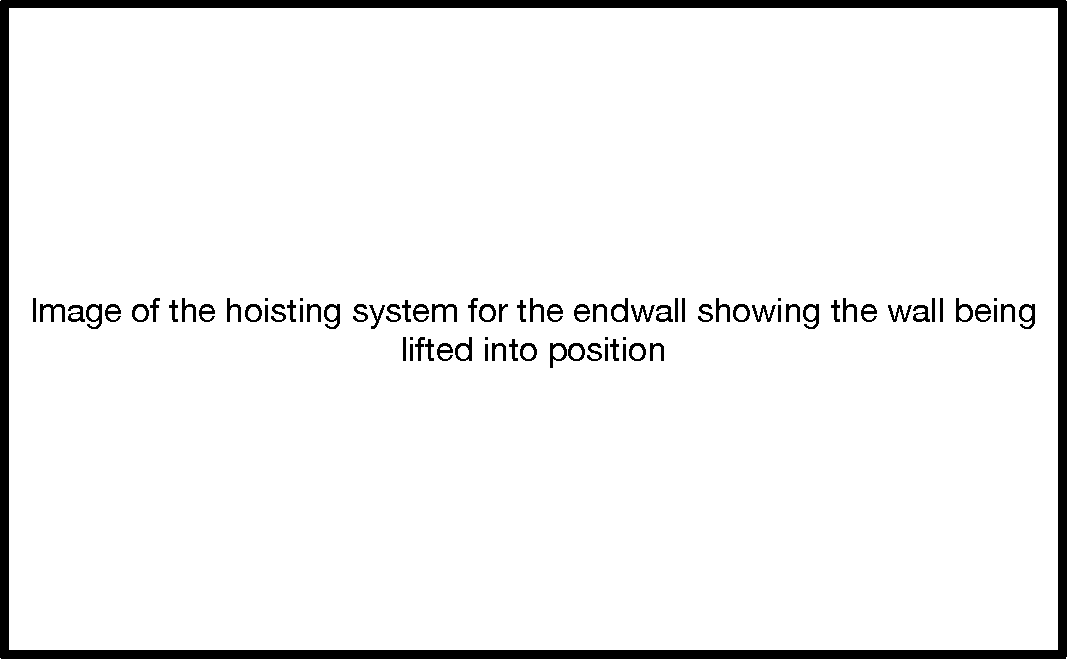
\includegraphics[width=.9\textwidth]{install-endwall-1}
\end{dunefigure}

The first detector equipment to be installed is the CISC thermometers and cameras at the East end of the cryostat which will be used to monitor the cool down, filling and commissioning of the detector. As these components are small the installation work can be performed using a scissor lift with 12 \si{m} reach. 
At present this is the tallest battery operated (thus cleanroom compatible) scissor lift rated for use in the US that we have identified.

The next step in detector installation is the field cage end-wall installation. 
The end-wall panels will be brought underground in custom crates as slung loads. 
Each of the 8 crates will hold 4 end-wall sub-panels and 8 sub-panels are needed to build one complete 12 \si{m} tall panel.  
The first step in the end-wall installation is to install a custom hoist to the end of the DSS beam. 
This will be used to lift and assemble the sub-panels in place. 
The end-wall transport crates will then be brought to the material airlock using a forklift where they are either un--crated or the crates are cleaned. 
Once clean the crates are moved into the cleanroom and placed next to the TCO. The a hoist running on the rails through the TCO is used to lift the endwalls into the cryostat.
Inside the cryostat the end-wall crates are moved into position using custom carts or simple pallet jacks.
The top Endwall sub-panel is then attached to the installation hoist and lifted out of the crate. When the sub-panel is free of the crate the cart is adjusted so the second sub-panel can be attached to the first and the pair are then again lifted. This process is repeated until the full 12 \si{m} Endwall field cage panel is assembles and can be attached to the DSS. 
Figure \ref{fig:install-endwall-1} shows an Endwall panel being lifted into position.
At this time all the HV connections inside the panel can be tested. The process is repeated for the four Endwall panels making up the East Endwall. 
In parallel to the endwall installation the cleanroom is configured for the installation of the APA and Cathode plane systems.

\begin{dunefigure}[Installation of the first Endwall]{fig:install-endwall-2}
  {The Endwalls are lifted out of the transport crates using the installation hoist. One panel is lifted then the next one is attached to the bottom. This is repeated until all eight panels are suspended from the installation hoist and then the panels are connected to the DSS.}
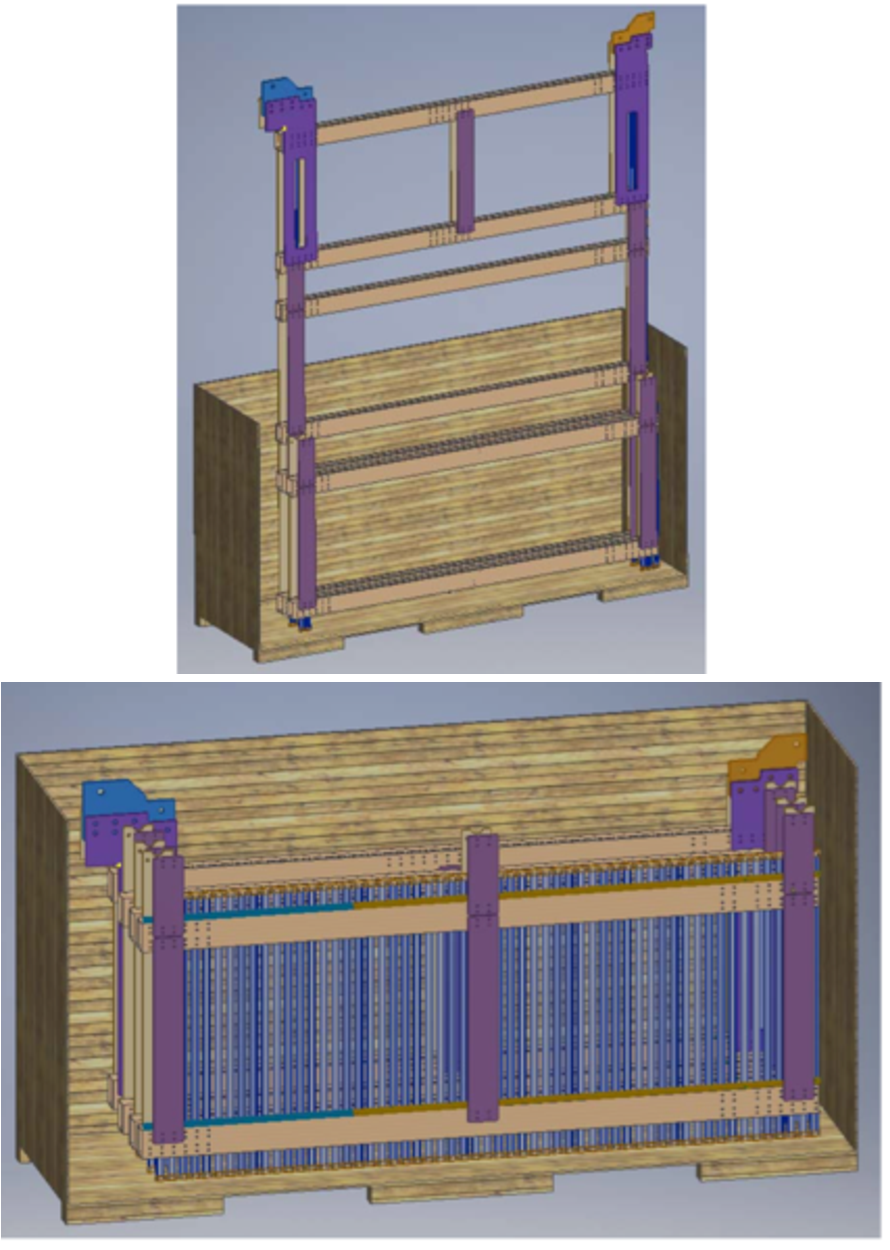
\includegraphics[width=.9\textwidth]{install-endwall-2}
\end{dunefigure}


The installation of the APA and Cathode with Top/Bottom Field cage modules is the most labor intensive period of the detector installation. If possible DUNE would like to finish installing one row of the APA, CPA, and FC modules every week. This represents the equipment shown in Figure \ref{fig:install-single-row}. To achieve this several separate teams will need to be working inside the cryostat positioning the equipment, connecting the cables, and deploying the field cages, while  other separate teams will be working in the outside cleanroom assembling the equipment and performing the final cold tests. The total time that would be needed to install a row of APA and CPA if all the work were to be done serially would be many weeks so performing the work as parallel  as possible will be very important for executing the installation efficiently. 


\begin{dunefigure}[Single row of APA and CPA]{fig:install-single-row}
{One row of the APA and CPA with associated field cages is shown. In this  image the field cages are deployed in the final orientation. The equipment in the figure represents $1/25$ of the total TPC.}
 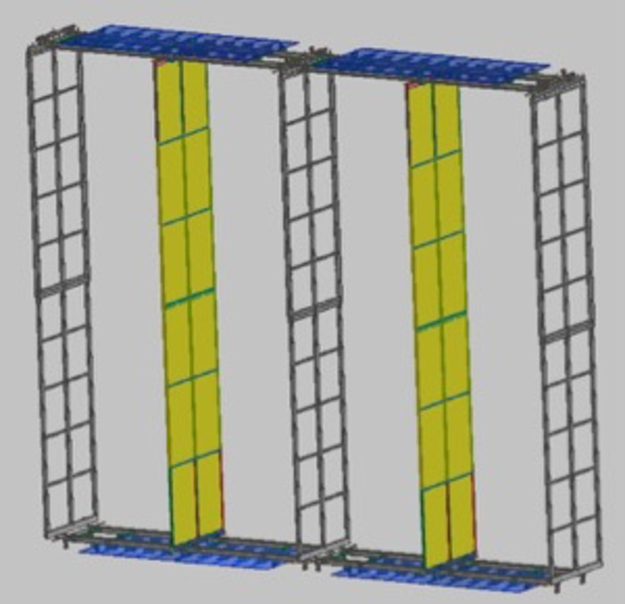
\includegraphics[width=0.5\textwidth]{install-single-row}
\end{dunefigure}

When the APAs are installed the area outside the cleanroom in the North cavern is available for storage and and it has capacity to store one full month of equipment. Equipment will be brought into the cleanroom's materials airlock through a rollup door in the West wall using either an electric forklift or electric pallet jacks.  The APAs enters the airlock in the transport crates which were used to bring the APAs down the Ross shaft and into the North cavern. Each transport box hold two APA with associated electronics and photon detectors and they enter the airlock in a horizontal or "landscape" orientation. Once inside the airlock the dirty outer panels of the transport box are removed, a section of the roof is opened and the bridge crane is used to lift the transport box into vertical. The airlock can then be cleaned and prepared for the APA assembly step where the upper and lower APA are assembled into a 12 \si{m} tall pair. The APA assembly sequence is shown in Figure \ref{fig:apa-assembly-v3}.


After initial visual inspection the lower APA is lifted out of the transport box again using the bridge crane and mounted on the APA assembly tower shown in green on the top row of images in in the Figure \ref{fig:apa-assembly-v3}. The  lower APA is supported from the bottom and guides connected to the sides of the APA provide mechanical stability while allowing the APA to be lifted using jacks integrated into the lower support. Next the upper APA is lifted out of the transport box and the transport box is removed from the airlock. The upper APA is connected to the transport rail above the APA assembly tower. At this point the upper APA is supported by the trolleys used for moving the APAs along the transport rails and it is stabilized using the APA assembly frame. The bridge crane is no longer needed after this step so airlock roof can be closed allowing the air to be purified. In order to assemble the two APA a metal linkage with electrical isolators is inserted into the upper APA and bolted into place. Then the lower APA is raised until the linkage can be bolted to the lower APA.  The APA pair can then be released from the assembly tower supports and jacks and is supported from the top APA to the rail system.
After the air quality in the airlock meets the requirements for ISO-8 and any dust covers are removed from the APA pair the APA can be moved into the cleanroom through a narrow vertical door in the cleanroom wall shown in brown in the top row of images in Figure \ref{fig:apa-assembly-v3}.


\begin{dunefigure}[APA assembly steps]{fig:apa-assembly-v3}
  {Top row from left:  \dword{apa} transport crate inside the airlock; \dword{apa} transport crate rotating to vertical position;  lower \dword{apa} placed on the \dword{apa} assembly frame; and upper \dword{apa} placed on the assembly frame. Bottom row right to left: \dword{apa} pair moving on the cleanroom transport rails; \dword{apa} in  position at the cabling tower; and the \dword{apa} being inserted into the coldbox.}
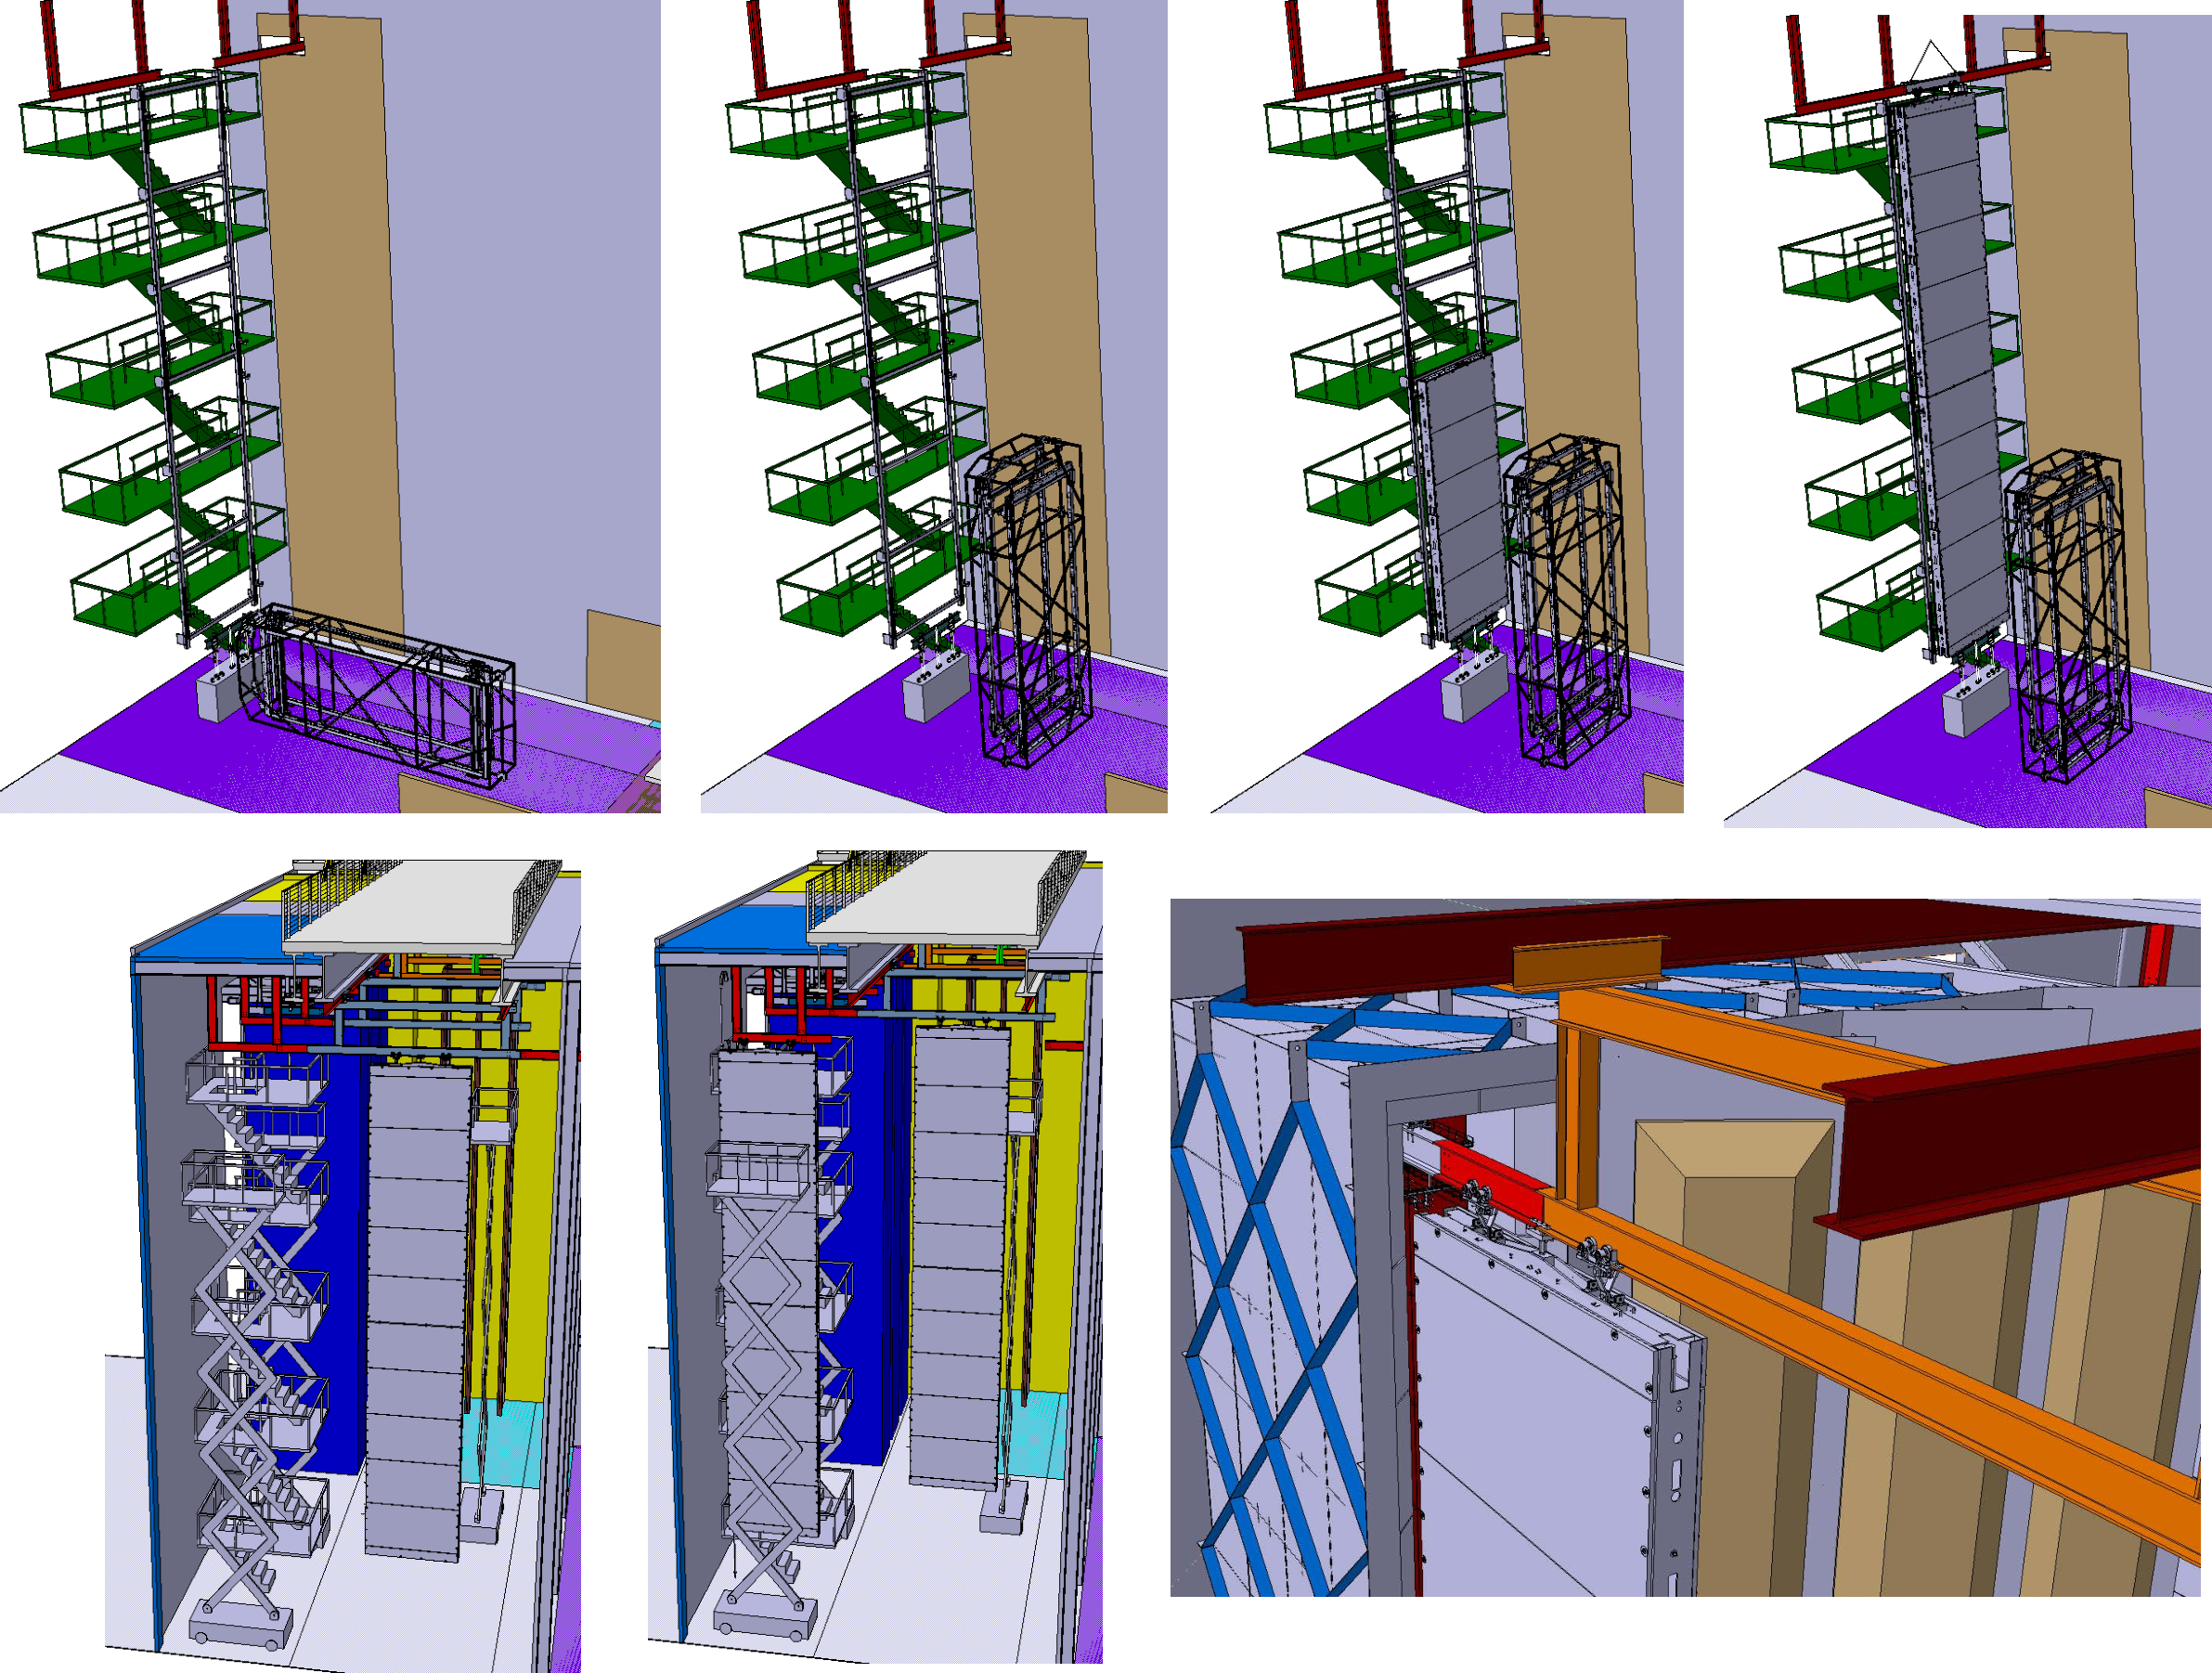
\includegraphics[width=.9\textwidth]{apa-assembly-v3}

\end{dunefigure}

The APA pair moves onto one of the shuttle beams in the cleanroom switchyard and can be moved north-south inside the cleanroom. The next assembly step is to install and test the electronics cabling. The APA is moved to line up with one of rails used to transport the APAs to the APA cabling tower. The lower left two image in Figure \ref{fig:apa-assembly-v3} shows the APA cabling tower in the cleanroom and an APA being moved into position. The APA cabling tower is capable of holding two APA pairs simultaneously allowing one APA pair to be cabled while a second APA undergoes electrical testing in parallel. In this position the cable trays and any other equipment needed during the cabling process can be installed. The electronics cables are delivered to the cleanroom on reels pre-bundled and tested. A lower APA reel is craned up to the top of the APA cabling tower and the cable is then spooled over to a motorized deployment spool and the cable guide is attached. The cable guide is then fed through a guide sieve and into the conduit on the side of the APA. The cable bundle is careful fed through the conduit and is anchored in place using a cryogenic compatible cable grip. The cable connected to the electronics at the bottom and is laid into the cable trays on top. This process is repeated for the second lower APA cable bundle. Finally the upper cables can be installed and prepared for transport. At this time a check of the functionality of all the electronics is performed. After the APA electrical test the APA pair is transported to a cold box where it undergoes a thermal cycle and complete system test. The APA being inserted into the coldbox is shown in the lower right image in Figure \ref{fig:apa-assembly-v3}. As the cold box is also a Faraday cage noise levels can be measure and the photon system checked for photon sensitivity. After the cold test is complete an APA will either move back to the cabling station if any repair is needed or it will be moved into the cryostat for installation. 



\begin{dunefigure}[CPA assembly steps]{fig:install-cpa-assembly}
  {The \dword{cpa} assembly steps are shown. Top row from left:  \dword{cpa} are delivered to the CPA assembly fixture in the cleanroom, the 3 \si{m} sub-panels are lifted onto the frame and connected. Bottom Row: After the CPA panel is complete it is moved into the room and the field cage modules are attached. The CPA is then moved into the cryostat.}
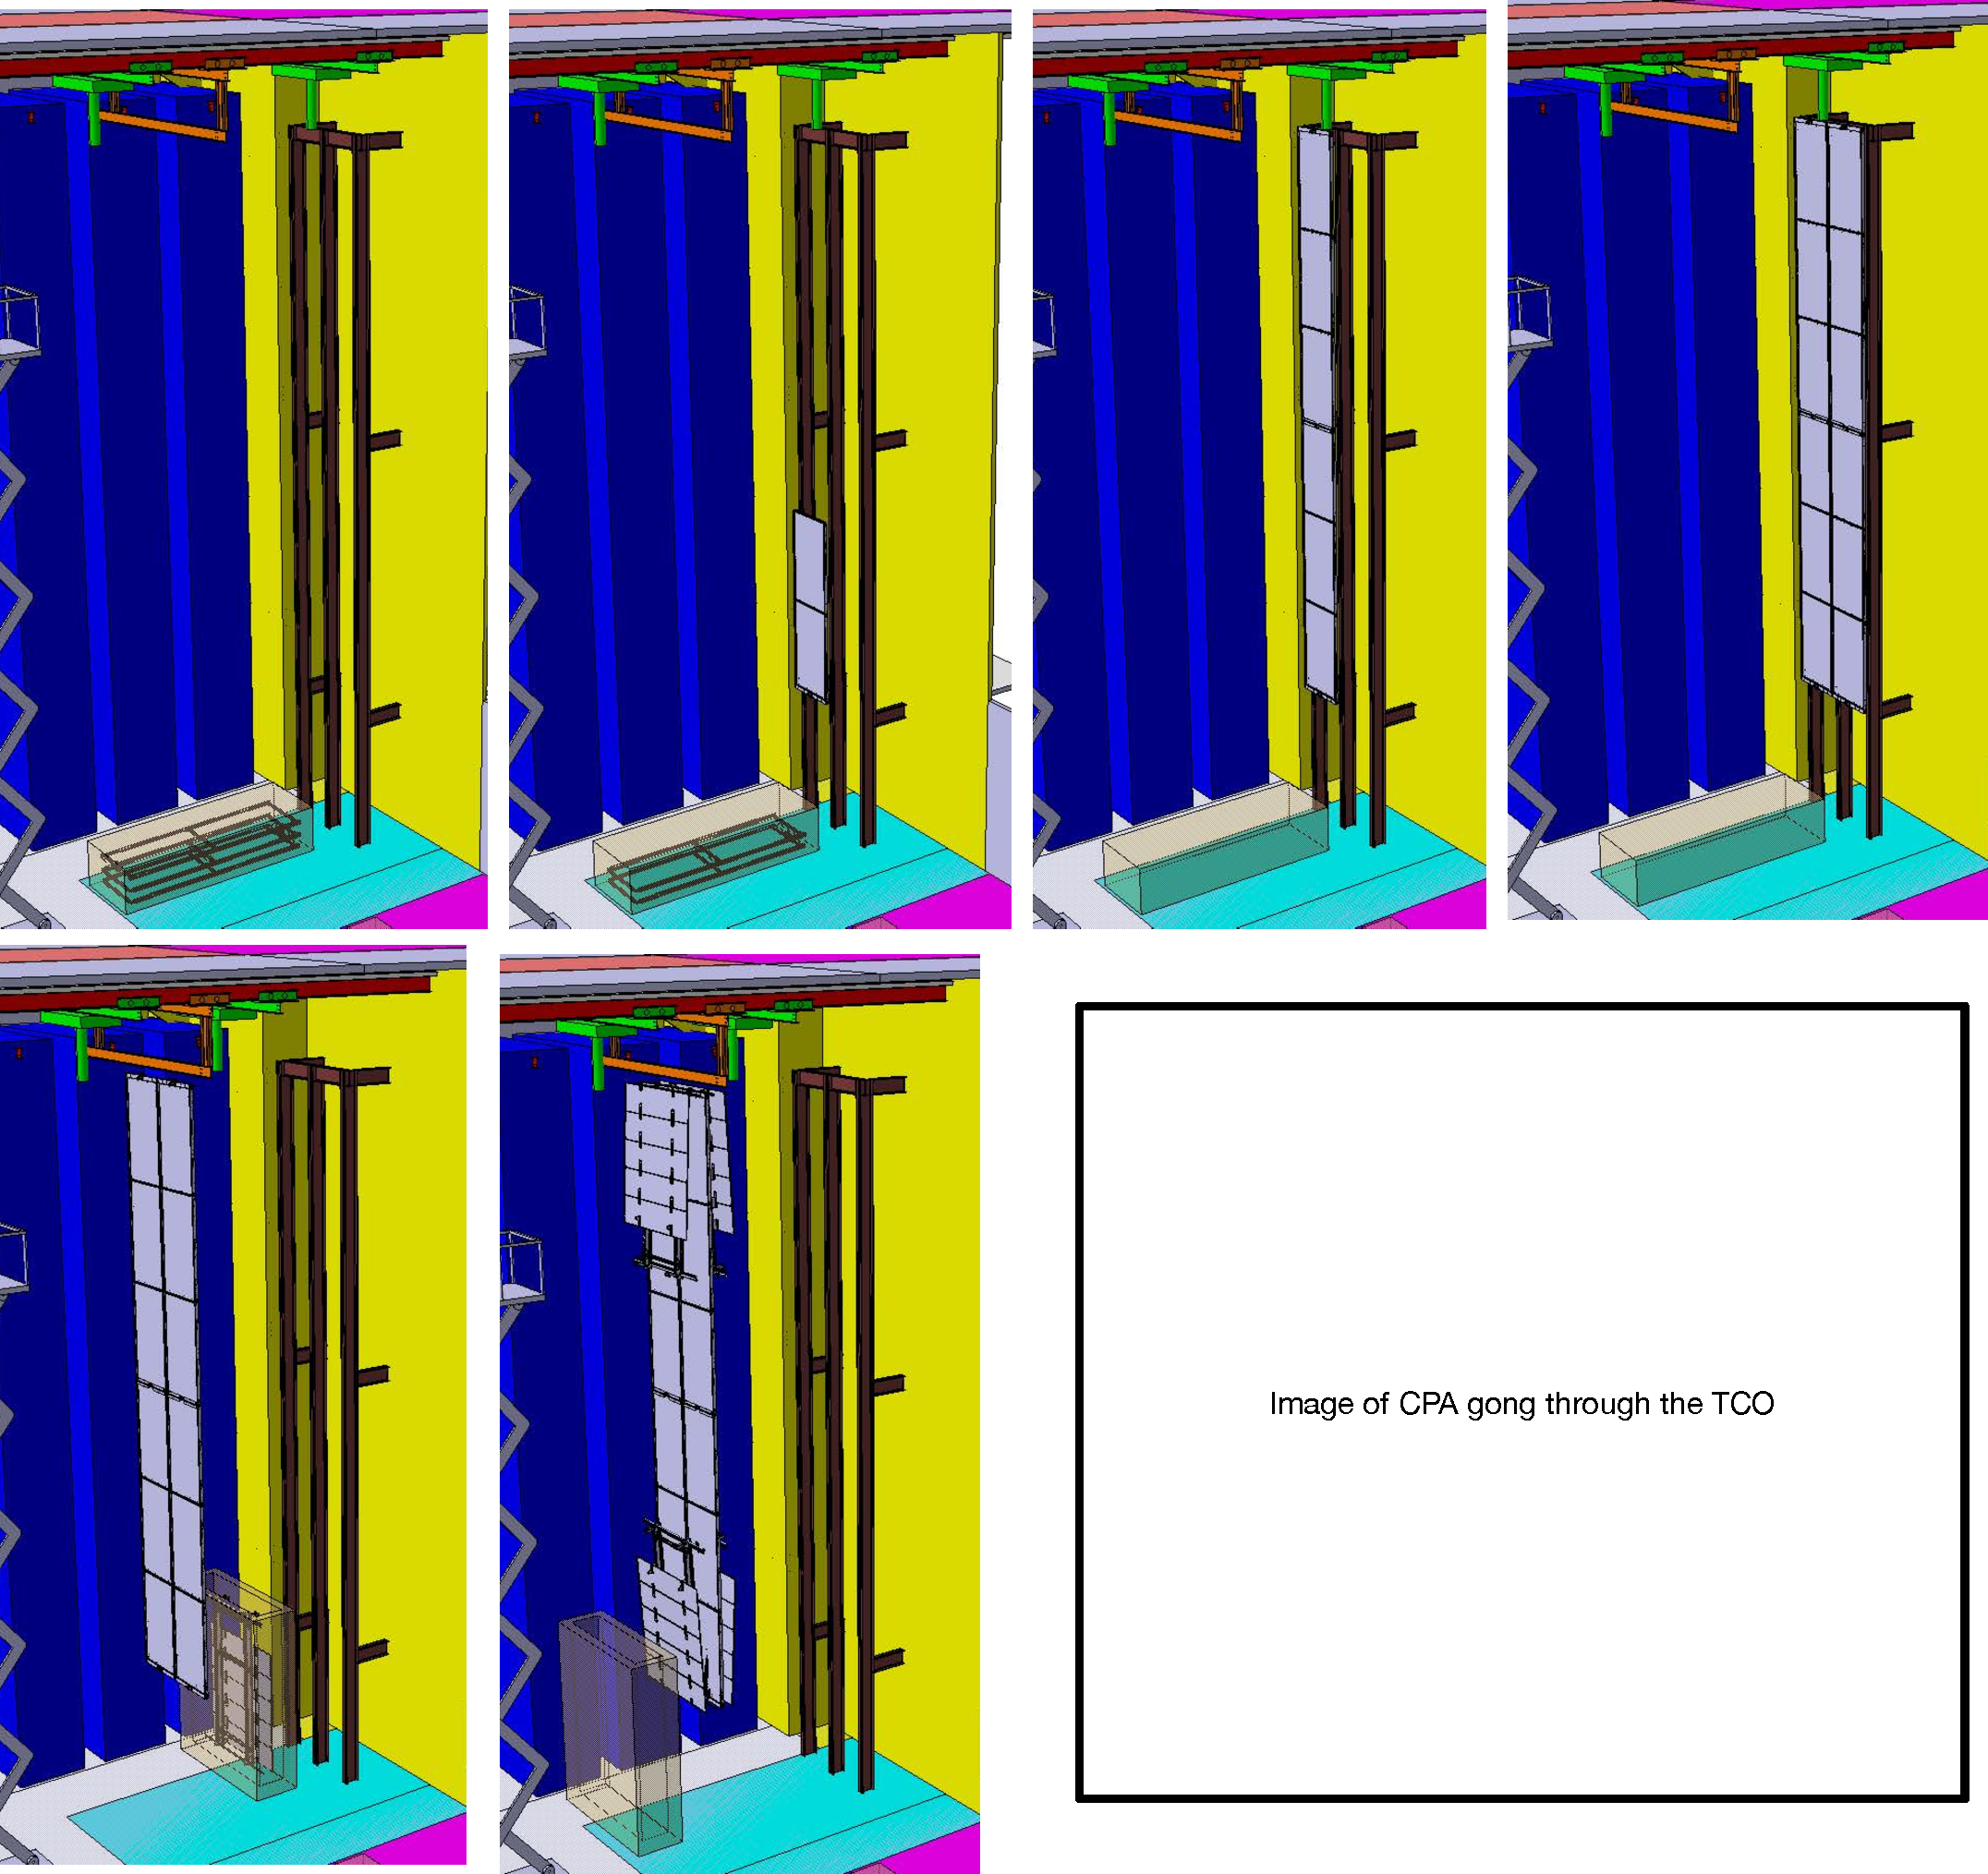
\includegraphics[width=.9\textwidth]{install-cpa-assemble}
\end{dunefigure}

The CPA and top/bottom field-cage modules are assembled in parallel to the APA assembly. Figure \ref{fig:install-cpa-assembly} shows the  assembly sequence. The sub-panels for the cathode plane are delivered to the airlock in crates which hold 3 \si{m} long 1.15 \si{m} segments. The crates after cleaning are brought into the cleanroom and opened. The panels inside are bagged to provide additional dust protection. The sub-panels are lifted out of the crate and place on the assembly frame using the cleanroom switchyard hoist. First one of the 1.15 \si{m} 3 
\si{m} tall sections are assembled and then the second one. Once the 2.3 \si{m} by 12\si{m} assembly is complete the assembly can be connected to the overhead rails with the support rods and trolleys. The assembled cathode panel is then moved away from the wall and the top field cage modules are attached. In Figure \ref{fig:install-cpa-assembly} the completed assembly is show with the lower field cage modules also attached. This is an option but present planning is to install the lower FC modules  inside the cryostat. Finally the CPA-FC assembly is moved into the cryostat.





Work inside the cryostat will proceed in parallel to the work in the outer cleanroom. 
The large detector components like APA pairs and CPA modules will enter the cryostat using the TCO rails which connect to the DSS switchyard.
Inside the cryostat the modules will be pushed onto one of the switchyard shuttle beams shown in  Figure \ref{fig:shuttle}. 
The DSS shuttle beam is then moved to the appropriate row of the DSS and then the module is pushed down the length of the cryostat into position. The position of the DSS beams are well defined and accurately surveyed so the APA and CPA modules can be accurately located by precisely positioning them along the DSS beams. A small correction in the height of the modules may be needed to accommodate deflections in the DSS due to load. Figure \ref{fig:install-ce-cables} shows the typical situation during the APA installation and cold electronics cabling. 

\begin{dunefigure}[Cold Electronics cabling inside the cryostat]{fig:install-ce-cables}
  {The installation of the APA and cabling of the cold electronics is described. In the left panel the situation is shown during the APA installation process. One row of APA and HV equipment is installed and a second APA is ready for the electrical cabling. In the top right image the cable trays are seen which will hold the CE cables and one of the workers in the scissor lift. In the left bottom image thework space is defined wiht the geometry of the APA the cryostat roof and the cable feedthru.}
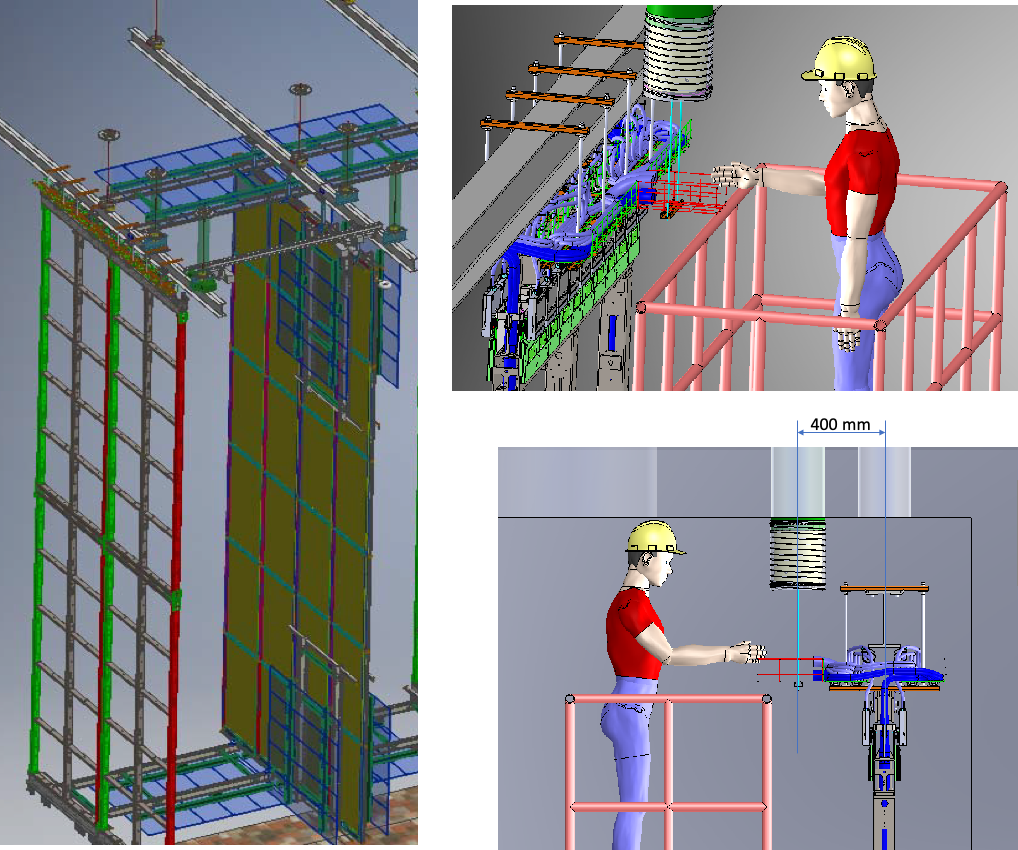
\includegraphics[width=.9\textwidth]{install-ce-cables}
\end{dunefigure}

After the APA is moved into position the permanent support rod is connected to the DSS beam and the trolleys are removed. The crawler used to push the APA along the rails is then moved back through the shuttle area and can be used for the next module. After the APA is locked in position the CE cabling can start. Even if a CPA module is already in position there is over 3 \si{m} space free between the APA and CPA so a scissor lift can easily be positioned in front to the APA. The two right images in Figure \ref{fig:install-ce-cables} show the situation at the top of the cryostat at during the cabling period. The cables are not shown so one can see the cable trays and their support infrastructure. At the start of the cabling all the cables are in the cable trays. A team of two people are in the scissor lift in front of the APA and  and a team of two people are on top of the cryostat. The cables from the bottom APA emerge from the side APA side-tube and are split into two bundles in the cable tray for a total of 4 cable bundles. The top APA also has the cables organized into 4 bundles. During the cabling process each bundle is partially removed from the cable tray and then fed up through the cable feedthru. At the top of the feedthru the cables are strain relieved and then the cables are strain releived again at the bottom of the crossing tube. This is repeated for each of the 8 cable bundles needed for the APA pair. When all the cable are installed through the cable tray Any excess length is returned to the cable tray at the top of the APA. On the roof the short individual cables are then connected to the feedthru flange and the electronics can be tested. When all the electronics and electrical connections are good the flange connecting the warm interface crate and can be sealed to the cryostat feedthru flange and the cable installation is complete. The electronics for each APA is continuously monitored after installation. 

\begin{dunefigure}[CPA assembly steps]{fig:install-cpa-fieldcage}
  {The steps to deploy the field cage modules after the \dword{cpa} is in position are shown. The field cage deployment tool is mounted above the DSS beams and a cable is connected to the top field cage module. The module is then lifted into position and latches to the APA module. The bottom APA is lowered using a wheeled cart that connects to the module with a rope. The module is then lowered using a pulley that is free to move on a slide and a winch.}
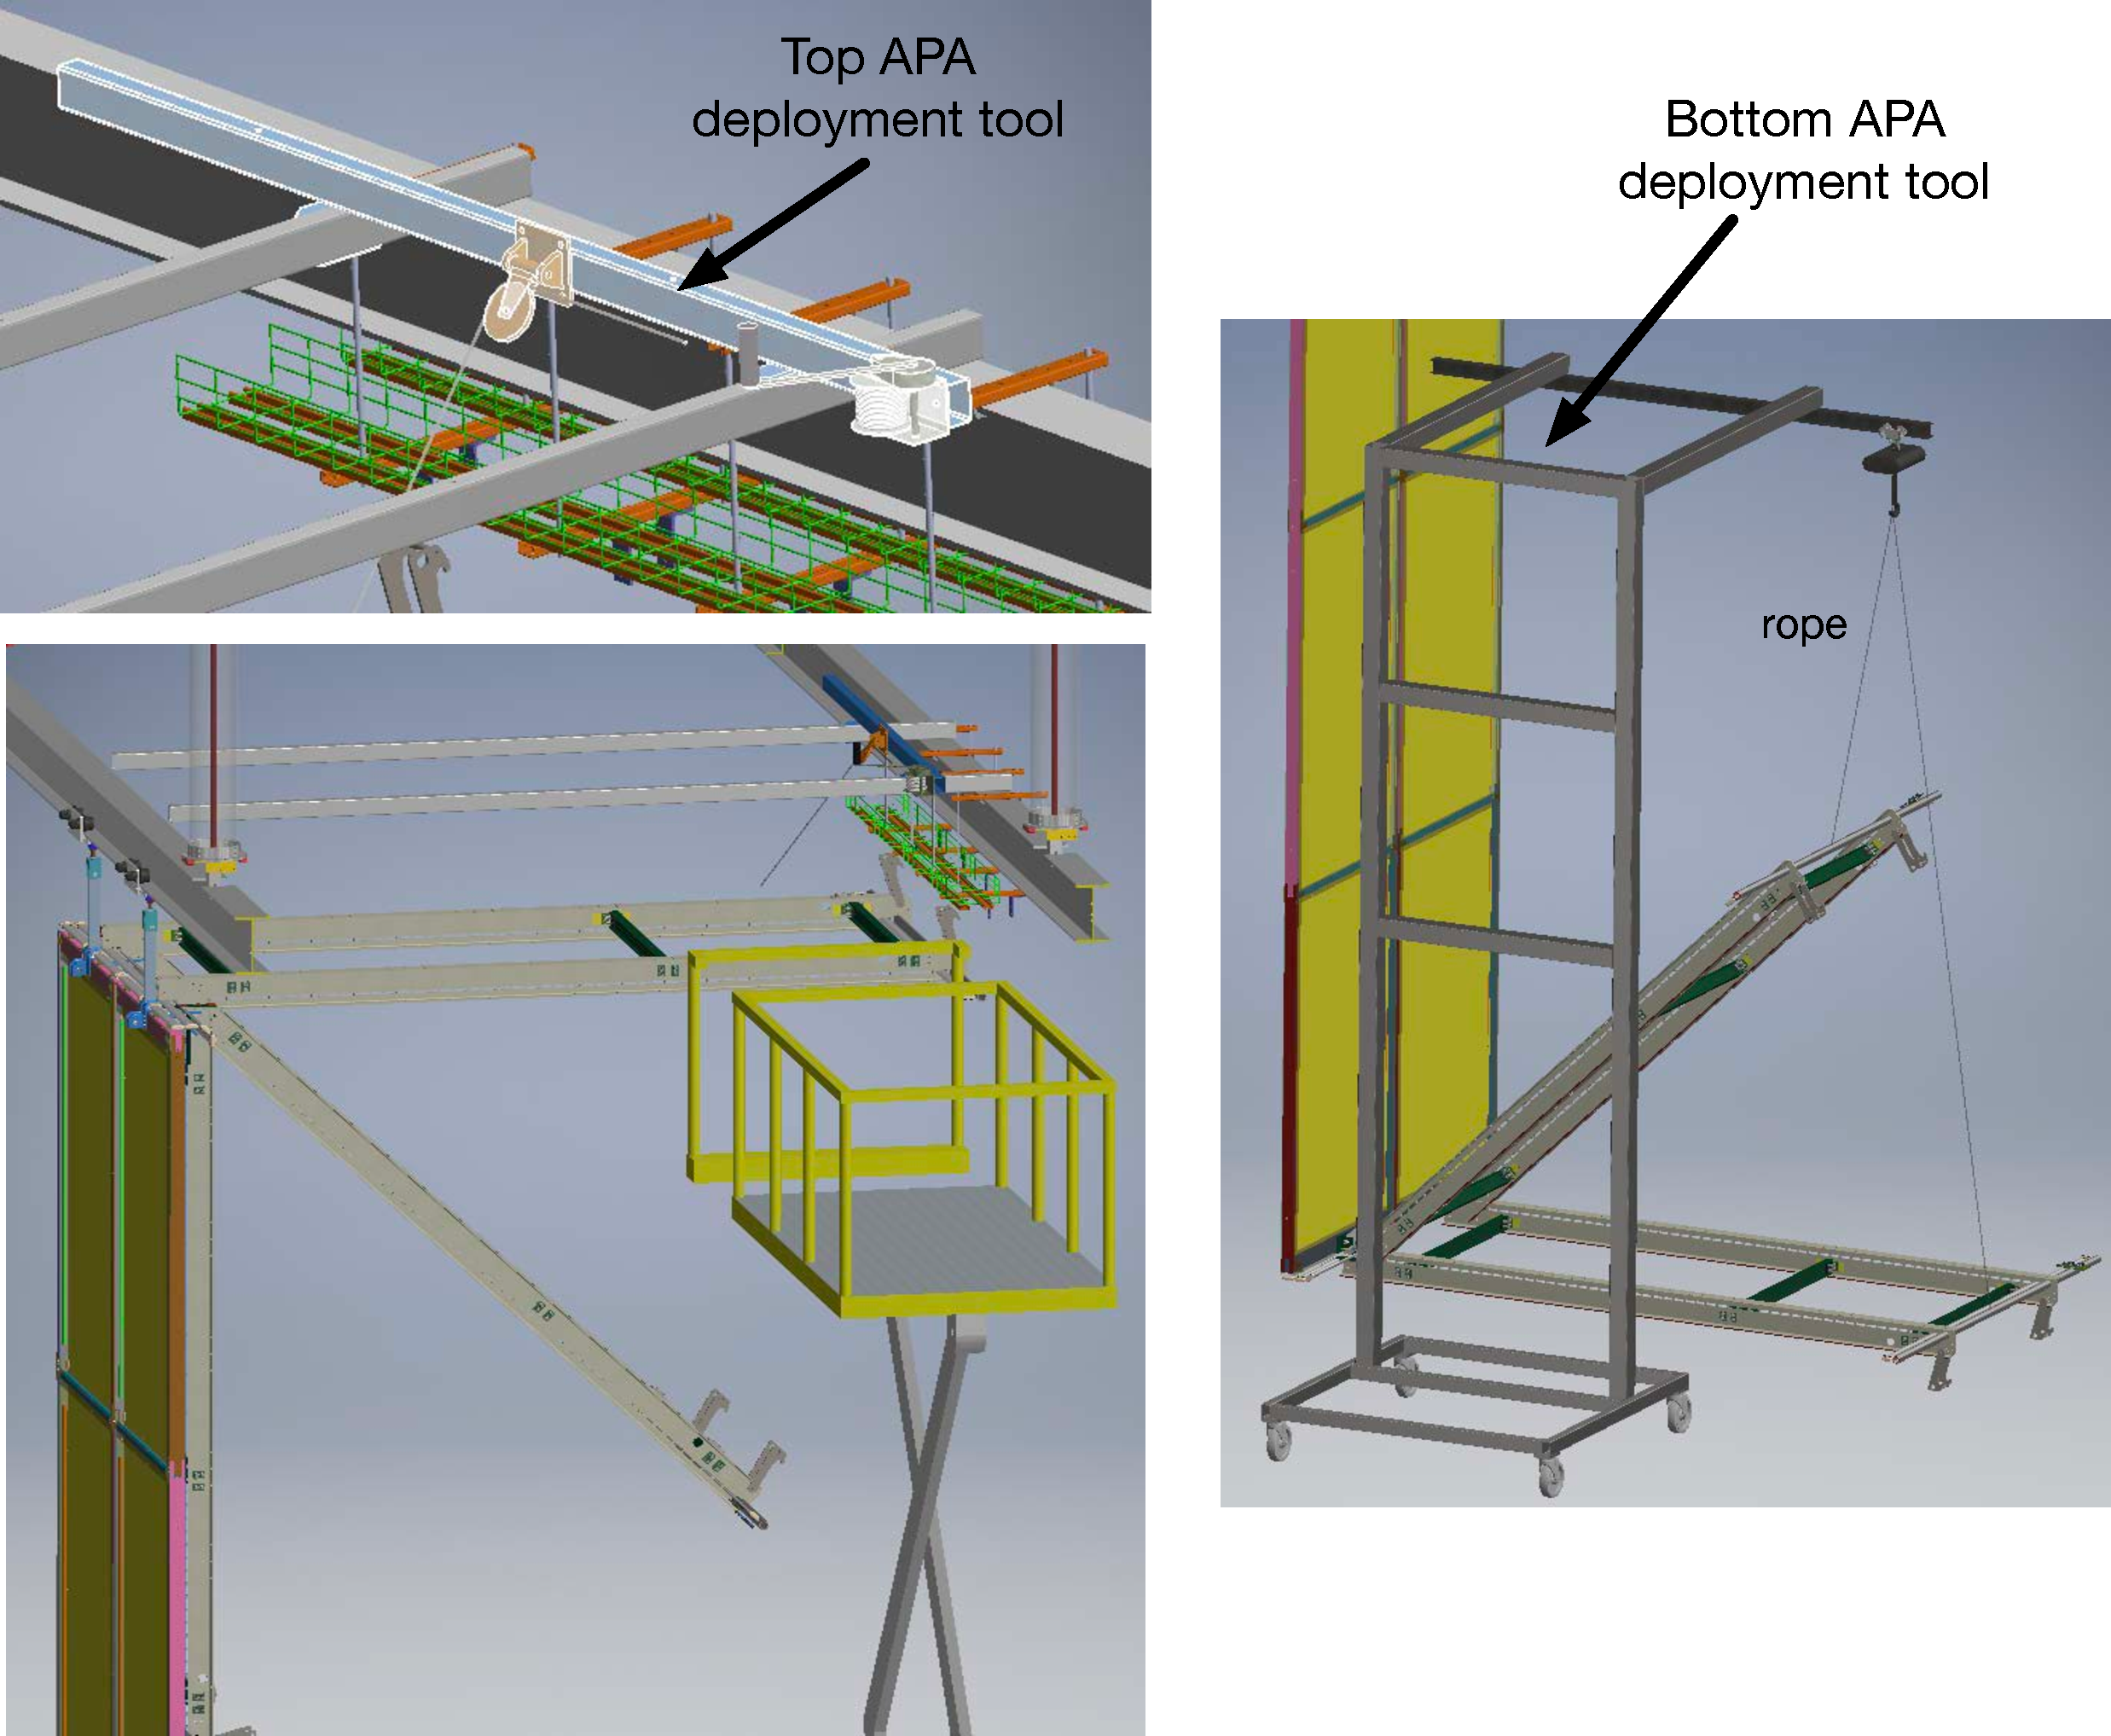
\includegraphics[width=.9\textwidth]{install-cpa-fieldcage}
\end{dunefigure}






% clear the figure buffer before starting the next session
\clearpage

\subsection{Detector Commissioning Phase}
\label{sec:fdsp-tc-inst-comiss}
After the \dwords{detmodule} is installed in the cryostat there remains a lot of work before it can be operated. 
First the \dword{tco} must be closed. 
This requires bringing back the cryostat manufacturer. 
First the missing panel with the steel beams and steel panel are installed to complete the cryostat's outer structural hull. 
Then the remaining foam blocks and membrane panels
are installed from the inside using the roof access holes 
to enter the cryostat. 

In parallel, the \lar pumps are installed at the ends of the cryostat and final connections are made to the recirculation plant. 
Once the pumps are installed, the cryostat is closed, and everything is leak tested, the cryogenics plant can be brought into operation. 
First the air inside the cryostat is purged by injecting pure argon gas at the bottom  at a rate such that the cryostat volume is filled uniformly but faster than the diffusion
rate. 
This produces a column of argon gas that rises through the volume and sweeps out the air. 
This process is referred to as the \textit{piston purge}. 
When the piston purge is complete the cool-down of the \dword{detmodule} can begin. 
Misting nozzles inject a liquid-gas mix into the cryostat
that cools the detector components at a controlled rate. 

Once the detector is cold the filling process can begin. 
Liquid argon stored at the surface  at \surf is vaporized and brought down the shaft in gaseous form and is then re-condensed underground. 
The \lar then flows through filters to remove any H$_2$O or O$_2$ and flows into the cryostat.
Given the very large volume of the cryostat and the limited cooling power for re-condensing, it is  expected to take \num{12} months to fill the first \dword{detmodule}. 
During this time the detector readout electronics will be on monitoring the status of the detector. 
Once the \dword{detmodule} is full, the drift high voltage can be carefully ramped up and data taking can begin.






\fixme{IDR text follows}




















\begin{dunefigure}[APA and CPA installation steps]{fig:Install-seq}
  {Top row from left:  crated \dword{apa} rotating to vertical position;  crated vertical \dword{apa} placed in cart; \dword{apa} panels moved to fixture using the under-bridge crane. Bottom row: series showing \dword{cpa} panels uncrated and moved to fixture. }
%\includegraphics[width=.9\textwidth]{apa-install-seq-top}
%\includegraphics[width=.9\textwidth]{cpa-install-seq-bot}
\end{dunefigure}

\begin{dunefigure}[\dword{cpa} and \dword{fc} unpacking and assembly]{fig:cpa-fc-unpack-assy}
  {On the left, the assembled \dword{cpa} panel is placed onto the north \dword{tco} beam. On the right, the (green) \dword{fc} panels (already lowered into \dword{sas} and moved into the clean room) are installed as the \dword{cpa} array hangs under the \dword{tco} beam. }
%\includegraphics[width=.9\textwidth]{cpa-fc-unpack-assy}
\end{dunefigure}

\begin{dunefigure}[\threed model of underground area showing installation infrastructure]{fig:Install-ISO-Top}
  {\threed model of the underground area showing the infrastructure to install the \dword{spmod} in cryostat~1. The most significant features are presented including the \dword{apa} and \dword{cpa} assembly areas, the region around the \dword{tco} for materials entering the cryostat,  the changing room, the region for the materials air lock, (\dword{sas}), 
  and the means of egress.}
%\includegraphics[width=.9\textwidth]{Install-ISO-Top}
\end{dunefigure}

\begin{dunefigure}[Section view of the \threed model showing layout]{fig:Install-TopView}
  {Section view of the \threed model showing layout, looking down on the installation area from below the bridge. Areas shown, left to right,  are the cryostat and \dword{tco}, the platform in front of the \dword{tco}, the dressing area, the \dword{apa} and \dword{cpa} assembly area (directly under the bridge), and the stairs and elevator. The lower right corner of the region is used as the materials air lock.}
%\includegraphics[width=.9\textwidth]{Install-TopView}
\end{dunefigure}





%The current installation plan is described. 
In the current installation plan, \dword{dune} will take
ownership of the different underground areas at different times. The
surface data room and the underground room in the \dword{cuc} are available
significantly before the collaboration has access to the cryostats; 
the optical fibers between the surface and underground will be in
place even earlier. This will allow a \dword{daq} prototype to be developed
and tested early. The installation of the \dword{daq} hardware can also be
finished before the start of detector installation if desired, so the
\dword{daq} will not be on the critical path.  When the collaboration receives
access to Cryostat~1 the steel work for Cryostat~2 will be
finished and the work on installing the membrane will have
started. Excavation will be complete.  For planning purposes it is
assumed that the first \dword{detmodule} will be \dword{sp} and the second
\dword{dp}. The first step in the \dword{sp} installation is to
install the cryogenics piping and the \dword{dss}. As this piping will
require welding and grinding, it is a dirty process and must be
complete before the area can be used as a clean room. When this is
complete the cryostat can be cleaned and the false floor
re-installed. The clean infrastructure for installing the \dword{detmodule},
including the clean room, work platforms, scaffolding, the
fixturing to hold the detector elements during assembly, and all the
lifts need to be set up. Once the infrastructure is in place and the
area is clean, the installation of the main elements can start. The
general layout of the installation area showing the necessary space
and equipment is shown in Figure~\ref{fig:Install-seq}. 

The \dword{spmod}  is installed by first installing the west endwall or
endwall~1 (see Figure~\ref{fig:endwall}).

\begin{dunefigure}[End view of \dword{spmod} with \dword{ewfc} in
  place]{fig:endwall}
  {End view of \dword{spmod} with \dword{ewfc} in
  place, with one row of \dwords{apa} and \dwords{cpa}.}
%\includegraphics[width=0.6\textwidth]{endwall.png}
\end{dunefigure}

The \dwords{apa} and \dwords{cpa} with top and bottom \dword{fc} panels are
installed next. The plan is to install six \dwords{apa} and four
\dwords{cpa} per week, which is enough to complete one of the \num{25}
rows every week. Additional time is built into the schedule to take
into account that the installation will be slower at the beginning and
some re-work may be needed. By building west-to-east, complete rows can
be finished and tested before moving to the next row. This reduces the
risk of finding a fault after final \dword{fc} deployment and cabling,
which would require dismantling part of the \dword{detmodule}. Some of the steps
needed to install the \dword{apa} and \dword{cpa} modules outside the
cryostat are also shown in Figure~\ref{fig:Install-seq}.  The middle three
panels show how the \dword{apa} needs to be handled in order to rotate
it and mount it to the assembly frame. After two \dwords{apa} are
mounted on top of each other, the cabling for the lower \dwords{apa}, and the
\dword{ce} and \dword{pd} cables can be installed. The
lower three panels show how the \SI{2}{m} \dword{cpa} sub-panels are
removed form the transport crates and assembled on a holding frame. Once
the \dword{cpa} module is assembled the \dword{fc} units can be
mounted. Finally, once the \dwords{apa} and \dwords{cpa} are installed,
the endwall~2 can be installed. A high-level summary of the schedule
is shown in Figure~\ref{fig:Install-Schedule}.

\begin{dunefigure}[High-level installation schedule]{fig:Install-Schedule}
  {High-level installation schedule.}
 %\includegraphics[width=\textwidth]{TP-Schedule-Feb2018.pdf}
\end{dunefigure}






For the \dwords{detmodule} to be installed in safe and efficient
manner, the efforts of the individual consortia must be coordinated
such that the installation is planned as a coherent process. The
interfaces between the individual components must be understood
and the spaces required for the installation process planned and
documented. The installation planning must take into account the
plans and scope of the \dword{lbnf} effort and the individual plans of
the nine consortia. By working with the \dword{lbnf} team and the
members of the consortia responsible for building and installing their
components, a joint installation plan and schedule, taking into account
all activities and needs of all stakeholders, can be developed. Although
the organization of the installation effort is still evolving, 
an installation coordinator will be the equivalent of a scientific lead for this effort.

One of the primary early responsibilities of the \dword{uit} is to
develop and maintain the \dword{dune} installation plan and the
installation schedule. This installation plan 
describes the installation process in sufficient detail to demonstrate
how all the individual consortium installation plans mesh and it 
gives an overview of the installation process. The installation plan
is used by the \dword{uit} to define the underground infrastructure
needed for detector installation and the interfaces it has with respect  to 
the consortia. The \dword{uit} is responsible for reviewing and
approving the consortium installation plans. Approved installation
plans, engineering design notes, signed final drawings, and safety
documentation and procedures are all prerequisites for the \dword{prr}. 
Approved procedures, safety approval, and
proper training are all required before the \dword{uit} performs
work. During the installation phase the installation leadership 
coordinates the \dword{dune} installation effort and adapts the schedule
as needed. The installation coordinator, together with management, will also
resolve issues when problems occur.







%%%%%%%%%%%%%%%%%%%%%%%%%%%%
\subsection{Installation Infrastructure}

The installation scope includes the infrastructure needed to install
the \dword{fd} such as the cleanroom, a small machine shop, special
cranes, scissor lifts, and access equipment.  Additional equipment
required for installation includes: rigging equipment, hand tools,
diagnostic equipment (including oscilloscopes, network analyzers, and
leak detectors), local storage with some critical supplies and some
personal protective equipment (PPE). The \dword{uit} will also provide
trained personnel to operate the installation infrastructure. The
consortia will provide the detector elements and custom tooling and
fixtures as required to install their detector components.





%%%%%%%%%%%%%%%%%%%%%%%%%%%%
\subsection{Prototyping and Testing (QA/QC)}
\label{sec:fdsp-tc-inst-qaqc}

\fixme{QA/QC Prototyping and testing}
\fixme{Include requirements; Lessons learned from ProtoDUNE-SP}
\subsubsection{Introduction}

\subsubsection{Ash River Testing}

Full scale mechanical testing of all the TCP components including the DSS are critical for the success of the Single Phase detector as shown from the \dword{protodune} experience. The NOvA Far Detector Assembly area at Ash River meets the criteria of both area and available equipment but also experienced technicians that helped construct the \dword{protodune} detector.  

\subsubsection{DAQ QC testing}

\subsubsection{APA QC testing}

\subsubsection{HV QC testing}
Steve Magill
\subsubsection{CE QC testing}
Marco
\subsubsection{CSIC QC testing}

\subsubsection{Photon QC testing}

These will set the schedule for the installation and will
determine the planning for staffing and budget. Having good estimates
for the time needed and having enough experience to ensure that the
interfaces are understood and the procedures are complete is important
for accurate planning. The experience at \dword{protodune} will be
very important as the \dword{protodune} installation establishes the
procedures for handling all the detector elements and in many cases
gives accurate estimates for the time needed. However, in the case of
the \dword{spmod}, many of these procedures need to revised or
newly developed. For example, the \dword{spmod} will be twice as high as
\dword{pdsp}, so two \dwords{apa} need to be assembled together
and a totally different cabling scheme is needed. Testing the
cabling must be done prior to the \dword{tdr} 
in order to
ensure the design is viable. The \dword{dp} will also need to develop
installation procedures as the \dword{dpmod} 
will have a significantly different \dword{fc} and cathode plane. 

By definition, the installation  is on the critical path, making it vital
that the work be performed efficiently and in a manner that has low
risk. In order to achieve this, a prototype of the installation
equipment for the \dword{spmod}  will be constructed at Ash
River (the \nova neutrino experiment \dword{fd} site in Ash River, Minnesota, USA), and the installation process tested with dummy detector
elements. It is expected that the setup will be available at the time
of the \dword{tdr}, but any lessons learned will need to be implemented and
tested after this. In the period just prior to the start of
installation, the Ash River setup will be used as a training ground for
the \dword{uit}.




%%%%%%%%%%%%%%%%%%%%%%%%%%%%
\subsection{Safety}
\label{sec:fdsp-tc-inst-safety}


%%%%%%%%%%%%%%%%%%%%%%%%%%%%
\subsection{Costs, Schedule and Risk Analysis}
\label{sec:fdsp-tc-inst-cost}

\subsection{Conclusions}
\label{sec:fdsp-tc-inst-concl}



The installation infrastructure to be provided by the \dword{uit}
includes: the underground ISO 8 (or class \num{100000}) clean room
used for the installation; cranes and hoists (if they are not
delivered by \dword{lbnf}); and scissor lifts, aerial lifts, and the common
work platforms outside the cryostat. The \dword{uit} will have
responsibility for operating this equipment and assisting the
consortia with activities related to rigging, material transport, and
logistics. Each consortium is responsible for the installation of
their own equipment, so the responsibility of the installation group is
limited, but the material handling scope is substantial. To support
the installation process, an installation floor manager will lead a
trained crew with the main responsibility of transporting the
equipment to the necessary location and operating the cranes, hoists,
and other common equipment needed for the installation. It is expected
that the installation crew will work with the teams from the various
consortia but will mainly act in a supporting function. The
\dword{uit} floor manager will be responsible for supervising the
\dword{uit} crew, but the ultimate responsibility for all detector
components remains with the consortia even while the underground
team is rigging or transporting these components.  This will be
critical in the case where any parts are damaged during transport or installation,
as the consortia need to judge the necessary actions. 
\fixme{judge the situation and determine the necessary actions?}
For this reason,
a representative or point of contact (POC) from the consortia must be
present when any work is performed on their equipment. The consortium
is responsible for certifying that each installation step is properly
performed.

The \dword{uit} acts as the primary point of contact with
\dword{lbnf} and \surf from the time the components reach the Ross
headframe until the equipment reaches the experimental cavern. If
something goes wrong, \surf calls the \dword{uit} leader who then
contacts the responsible party. The consortia are responsible for
delivering to the \dword{uit} all approved procedures and specialized
tooling required for transport. The \dword{uit} leader acts as a point
of contact if the \dword{lbnf} or \surf team has questions or difficulties
with the underground transport.  The \dword{uit} receives the
materials from \dword{lbnf} and \surf at the entrance to the \dword{dune}
excavations. The \dword{uit} then delivers the equipment to the
required underground location.



%DAVID added cryo cold box??%%
%%{Cold Boxes Cryogenics}
\label{sec:fdsp-tc-cryocoldbox}

%The cryogenics supporting the \coldbox{}es underground must ensure reliable and safe operation of the system used to test the \dwords{apa} that will be installed inside the cryostats. The main functional requirements of the system are
The  \coldbox{}es will be used to test the \dword{apa}s underground prior to installation. % in the cryostat. 
The cryogenics supporting the \coldbox{}es  must ensure their reliable and safe operation; to that end, it must
\begin{itemize}
\setlength\itemsep{1mm}
\setlength{\parsep}{1mm}
\setlength{\itemsep}{-5mm}
\item support three \coldbox{}es operating in parallel: %for testing dual \dword{apa}s: 
one in \cooldown mode, two either in steady-state or warm-up modes.
\item allow personnel in the cleanroom during all phases of the purge, \cooldown, operation, and warm-up modes. 
\item test the detector modules at near \dword{lar} temperature.
\item operate 24 hours a day, seven days a week for 10 years.
\item allow remote operations.
\item be located in the vicinity of the \dword{tco}. Space is available on top of the cryogenic mezzanine on the roof of the cryostat.
\end{itemize}

It must operate in the following modes: %fulfill the following modes of operations:

\begin{itemize}
\setlength\itemsep{1mm}
\setlength{\parsep}{1mm}
\setlength{\itemsep}{-5mm}
\item \textbf{purge}: During this mode, air is removed from the system (\coldbox and cryogenic system) and replaced with dry nitrogen. The concentration of moisture is monitored, and when it no longer decreases, the \cooldown can commence.
\item \textbf{\cooldown}: Cold nitrogen is introduced into the system to cool the inside of the \coldbox and the \dword{apa} inside it. %it down and to cool down the detector contained inside the coldbox. 
This should take 24 hours, during which time the temperature decreases from room temperature to about \SI{90}{K}. 
\item \textbf{steady-state operations}: After reaching %the nominal temperature of 
approximately \SI{90}{K}, %the value is maintained for 48 hours, during which 
the detector is turned on and fully tested. % at cold. 
This takes about 48 hours.
\item \textbf{warm-up}: After completing the test, the system is %slowly 
warmed up to room temperature over a period of 24 hours. %This should take 24 hours, during which the temperature goes from approximately \SI{90}{K} to room temperature.
\end{itemize}

\begin{dunetable}
[\Coldbox  cryogenics system parameters] %for specifications]
{lc}
{tab:table-cryo-coldboxes}
{Table of parameters for the \coldbox cryogenics system.}
Parameter & Value 
\\ \toprowrule
Dual \dword{apa} thermal mass &  1,600 kg\\ \colhline
Temperature uniformity & $+60$ K / $-0$ K \\ \colhline
Electronics load & 300 W \\ \colhline
\Coldbox insulation thickness &  0.3 m \\ \colhline
Target \cooldown temperature &  \SI{90}{K} \\ \colhline
Target \cooldown duration &  24 hr \\ \colhline
Target steady-state duration &  48 hr \\ \colhline
Target warm-up duration &  24 hr \\ \colhline
Maximum cooling power  &  \SI{13}{kW}  \\ \colhline 
Maximum liquid nitrogen consumption  &  \SI{300}{l/hr}  \\ \colhline 
\end{dunetable}

The evaporation of liquid nitrogen provides the cooling power for the system. Warm nitrogen and a heater provide the heating power. At peak consumption, the expected maximum heat load is \SI{8.5}{kW}. Assuming a 50\% margin on the refrigeration load, the cryogenics system requires \SI{13}{kW} of net cooling power at peak consumption, which equals about \SI{300}{l/hr} of evaporating liquid nitrogen.

Two layouts are currently under consideration: (1) a closed loop with mechanical refrigeration, in which liquid nitrogen is generated {\it in situ}, circulated, and the spent nitrogen recondensed before being put back into the system; and (2) open loop, in which liquid nitrogen is transported underground by means of portable dewars, circulated, and the spent nitrogen vented away. For the closed loop, we would need a mechanical refrigeration capable of supplying \SI{13}{kW} of cooling. For the open loop, it is possible to use a \SI{2000}{l} dewar, which is commercially available and transportable up and down the Ross Shaft inside the cage. To supply the required amount of nitrogen, four trips per day are needed.

The current versions of the closed loop and open loop systems are presented in Figures~\ref{fig:mechanical-refrigeration} and~\ref{fig:LN2}, respectively. % . The current version of the open loop system is presented in Figure~\ref{fig:LN2}.

\begin{dunefigure}[\Coldbox cryogenics support system based on mechanical refrigeration ]{fig:mechanical-refrigeration}
  {Layout of the cryogenics supporting the \dword{apa} test facility with mechanical refrigeration (closed loop).}
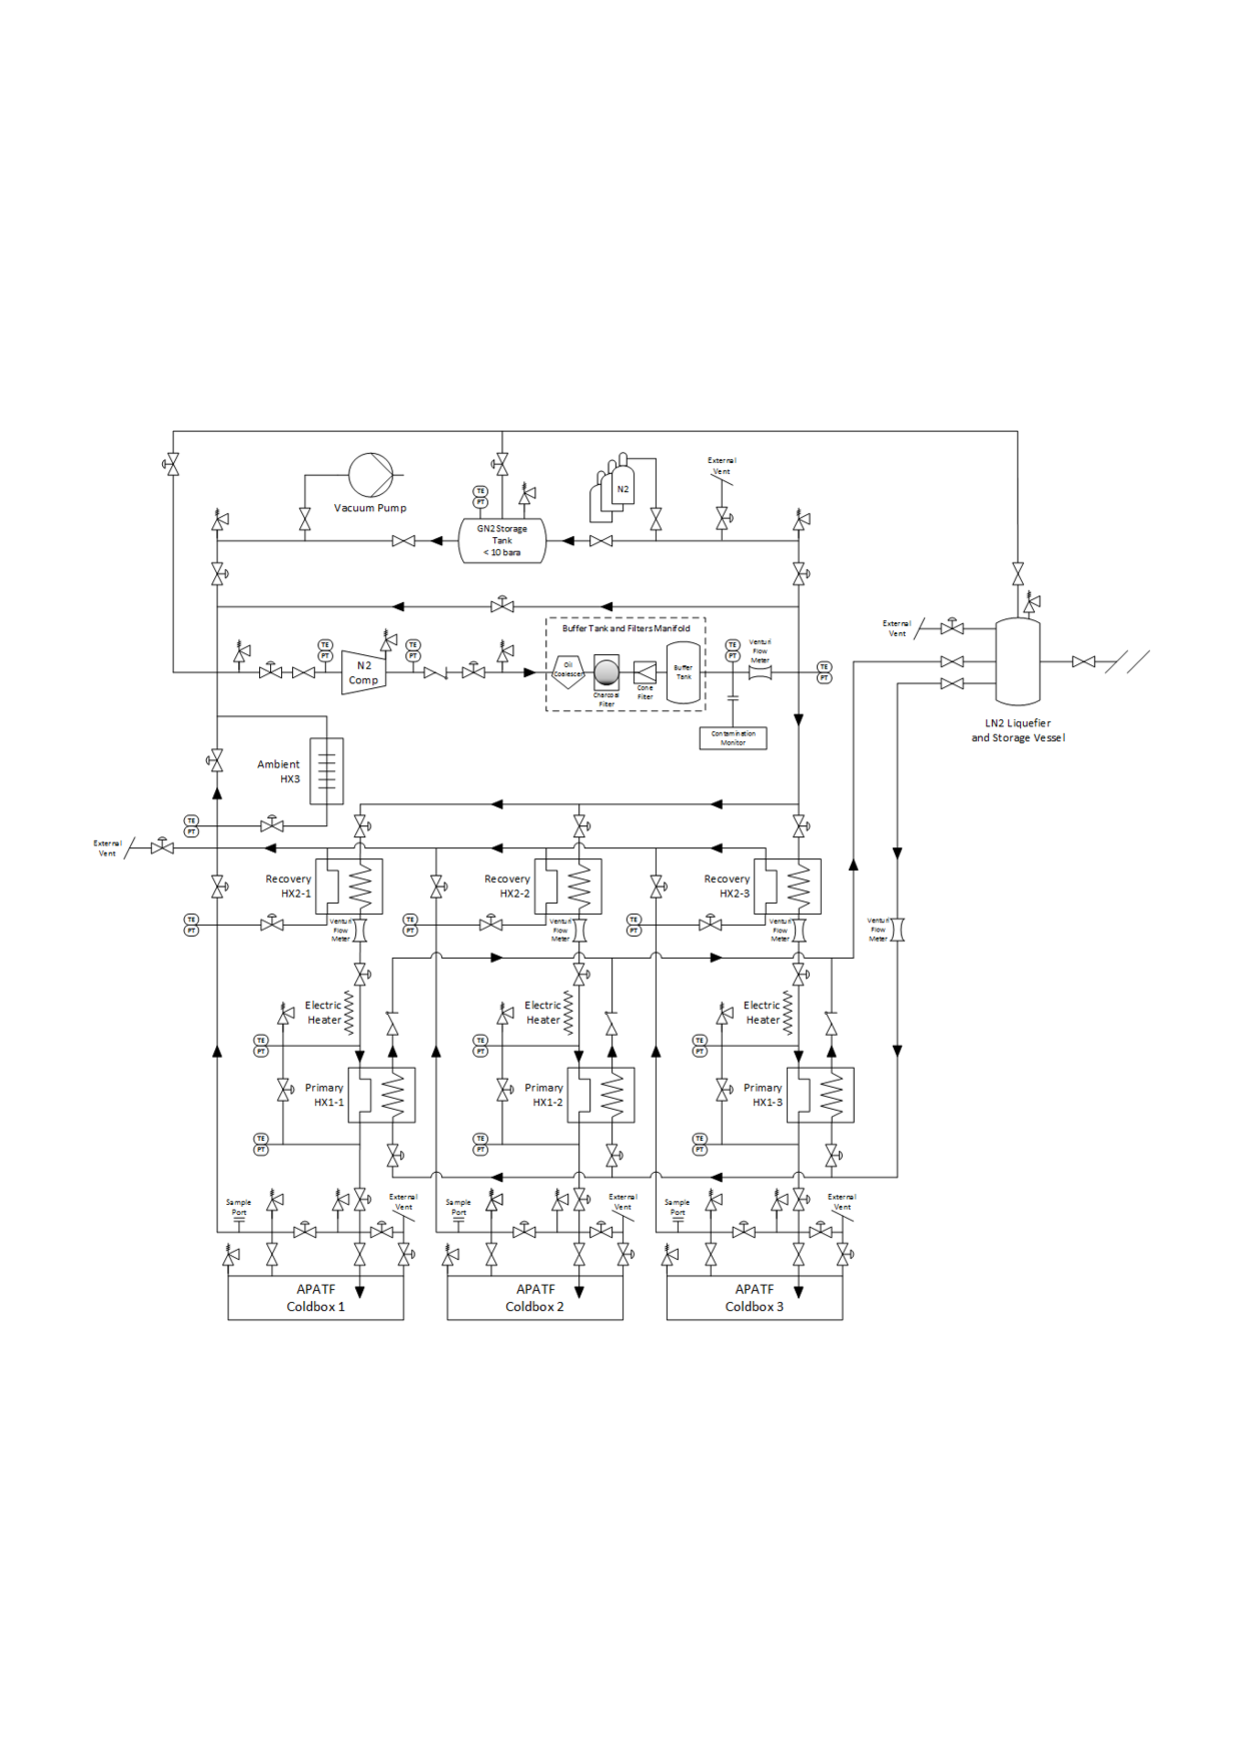
\includegraphics[width=.98\textwidth]{graphics/Cryo-cold-box-mechanical.pdf}
\end{dunefigure}

\begin{dunefigure}[\Coldbox cryogenics support system based on LN2 ]{fig:LN2}
  {Layout of the cryogenics supporting the \dword{apa} test facility with open loop refrigeration (open loop).}
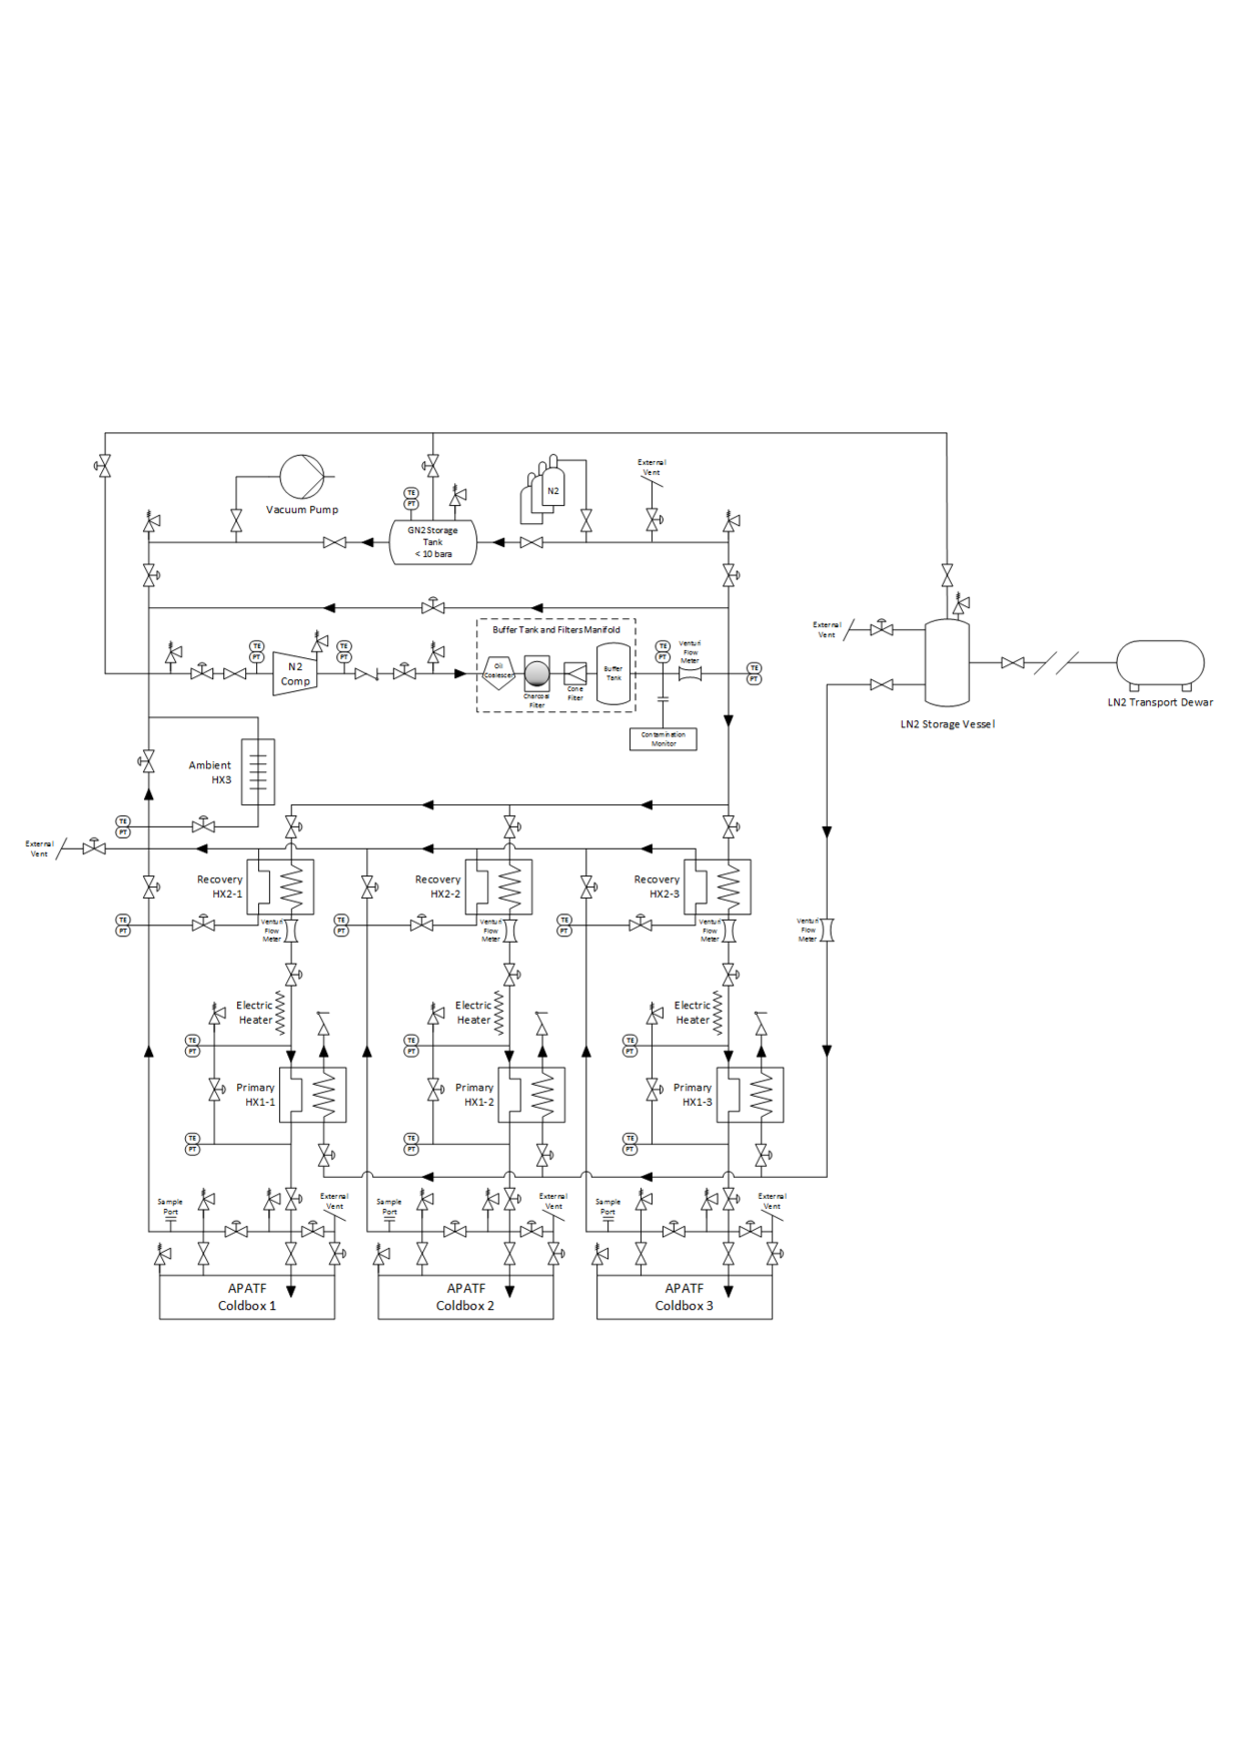
\includegraphics[width=.98\textwidth]{graphics/Cryo-cold-box-LN2.pdf}
\end{dunefigure}



%%%%%%%%%




 
 



